\documentclass[12,twoside]{mammeTFM}
%\usepackage[active]{srcltx}
\usepackage{amsthm,amsmath,amssymb,amsfonts,amscd}
\usepackage{graphicx}
\usepackage{enumerate}
\usepackage[all]{xy}
\usepackage{booktabs}
%\usepackage[usenames]{xcolor}
%\usepackage{fancyhdr}

%%%%%Author packages if necessary


% Theorem Environments: add extra ones at the end if you need it.

\newtheorem*{theoremA}{Theorem A}
\newtheorem{theorem}{Theorem}[section]

\newtheorem{proposition}[theorem]{Proposition}
\newtheorem{lemma}[theorem]{Lemma}
\newtheorem{corollary}[theorem]{Corollary}
\newtheorem{conjecture}[theorem]{Conjecture}

\theoremstyle{definition}
\newtheorem{definition}[theorem]{Definition}
\newtheorem{example}[theorem]{Example}

\theoremstyle{remark}
\newtheorem{remark}[theorem]{Remark}
\newtheorem*{remarknonumber}{Remark}
\newtheorem{observation}[theorem]{Observation}




%%%%%%%%%%%%%%%%%%
% macros/abbreviations: Include here your own.
%%%%%%%%%%%%%%%%%%

\newcommand{\N}{\ensuremath{\mathbb{N}}}


% Body of document

\titol{Why the non-monotonicity of excellence\\[3mm] f***** up my life}
\titolcurt{Regularity Lemmas for Stable Graphs}
\authorStudent{Severino Da Dalt}
\supervisors{(Lluis Vena Cros)}
\monthYear{February, 2025}

%\msc[2010]{Primary  	55M25, 57P10, Secondary 55P15, 57R19, 57N15.}

\paraulesclau{regularity, stable graphs, graph theory, ...}
\agraiments{
Thanks to...}


\abstracteng{This should be an abstract in english, up to 1000 characters.}




%%%%%%%%%
\begin{document}

\maketitle

% sections
\section{Introduction} \label{sec:introduction}

    \subsection{Szemerédi's Regularity Lemma}

        Szemerédi's Regularity Lemma (SzRL)~\cite{regular_partitions_of_graphs} is a powerful tool in graph theory,
        stating that every graph can have its vertex set decomposed into an equitable partition such that most,
        but not all, pairs of parts are \emph{regular}.
        A regular pair is one whose edge distribution resembles that of a random bipartite graph (in the sense of
        satisfying its expected properties).
        The strength of the quasi-random properties is measured with the regularity parameter $\epsilon$.

        % \subsection{Applications}
        This theorem has seen many applications in a wide variety of areas of mathematics
        (see an early survey from the mid 1990's~\cite{the_regulariy_lemma_and_its_applications_in_graph_theory}),
        such as graph
        theory~\cite{proof_of_the_alon–yuster_conjecture,
            on_universality_of_graphs_with_uniformly_distributed_edges,
            hamilton_decompositions_of_regular_expanders_applications,
            proof_of_a_tiling_conjecture_of_komlos,
            the_approximate_loebl_komlos_sos_conjecture_IV,
            the_approximate_loebl_komlos_sos_conjecture_III,
            the_approximate_loebl_komlos_sos_conjecture_II,
            the_approximate_loebl_komlos_sos_conjecture_I}\footnote{Aside from the results that directly apply the SzRL,
            there are many that either use suitable variants of SzRL or are deeply inspired by its ideas.},
        limits of dense graphs~\cite{convergent_sequences_of_dense_graphs_I,
            convergent_sequences_of_dense_graphs_II,
            szemeredis_lemma_for_the_analyst,
            regularity_partitions_and_the_topology_of_graphons} (see the book~\cite{large_networks_and_graph_limits}),
        number theory~\cite[Szemerédi's Theorem]{on_sets_of_integers_containing_k_elements_in_arithmetic_progression},
        and Ramsey Theory~\cite{threshold_functions_for_ramsey_properties,
            three-color_ramsey_numbers_for_paths,
            ramsey_turan_theory,}, to name a few.
        The regularity method has also been generalized to hypergraphs~\cite{
            regularity_lemma_for_k_uniform_hypergraphs,
            regular_partitions_of_hypergraphs_regularity_lemmas,
            the_counting_lemma_for_regular_k_uniform_hypergraphs,
            a_variant_of_the_hypergraph_removal_lemma,
            hypergraph_regularity_and_the_multidimensional_szemeredi_theorem}.
        Also, it has seen important applications to computer science, such as in property testing (see~\Cref{subsec:subsection_1.3}).
        This brief summary is by no means an exhaustive list of the many applications that has seen the Regularity Lemma as
        a key component.

        % \subsection{Problems with SzRL}
        Since this result is applicable to \emph{any} graph and the number of parts of this partition with good properties is constant,
        it should not be surprising that some limitations arise.
        Firstly, not necessarily all pairs are regular, but most crucially, the required upper bound on the number of
        parts is, although constant, very large.
        More specifically, it is a tower of exponentials (it has the form $2^{2^{2^{\text{\reflectbox{$\dots$}}}}}$)
        whose height depends on the regularity parameter $\epsilon$.

        In the general setting, both limitations have been proven to be unavoidable.
        In~\cite{lower_bounds_of_tower_type_for_szeremedis_uniformity_lemma}, Gowers shows that there exists a family of graphs
        for which the lower bound on the number of parts is still a tower of exponentials\footnote{
        To be more specific, the author shows that the number of parts is lower bounded by an exponenetial tower of $2$'s where
            the height of the tower is at least proportional to $\log\parround{1/\epsilon}$.
            Meanwhile, in the usual proof of the theorem, the upper bound on the height of the tower is proportional to
            $\epsilon^{-5}$.
        }.
        On the other hand, it is folklore knowledge that large-enough half-graphs present irregular pairs in any
        regular partition (\cite{irregular_pairs_in_half_graphs_szemeredi_regularity} gives a written proof of this fact).
        Having seen this unavoidability, it is natural to ask for the underlying reasons of those limitations and which
        additional conditions can be imposed or levied so that the parameters can be improved.

    \subsection{Versions of SzRL}

        In order to reduce the bound on the number of parts, one can relax the property required on the partition.
        One of the first successful implementations of such approach was given
        by~\cite[Theorem 12]{quick_approximation_to_matrices_and_applications} which is now known as
        \emph{the weak regularity lemma}.
        Towards the other direction one can strengthen the property on the
        partition~\cite[Lemma 4.1]{efficient_testing_of_large_graphs}, at the cost of increasing the number of parts.
        This is known as the \emph{strong regularity lemma} and it is particularly useful when working with induced
        subgraphs (more on this in \Cref{subsec:subsection_1.3}).
        The previous results can be thought as three instances of a family of regularity lemmas, with varying
        strength~\cite{regularity_partitions_and_the_topology_of_graphons, szemeredis_lemma_for_the_analyst}.
        This is hinted in~\cite[Lemma 4.1 and its discussion]{szemeredis_lemma_for_the_analyst}, and for example, an even
        stronger instance in this family is given explicitly in~\cite[Section 5.1 - pg. 439]{regularity_partitions_and_the_topology_of_graphons},
        where is referred to as an \emph{ultra-strong} regularity lemma.

        % \subsection{Subclasses versions}
        Now, another way of tackling the limitations of the SzRL is to reduce the scope to an appropriate subclass of graphs.
        A relevant example of this approach is the class of graphs with bounded VC-dimension;
        the notion of VC-dimension was firstly introduced by Vapnik \& Chervonenkis
        in~\cite{the_uniform_convergence_of_frequencies_of_the_appearance_of_events_to_their_probabilities}
        \hspace{-3pt}\footnote{
            See~\cite{on_the_uniform_convergence_of_relative_frequencies_of_events_to_their_probabilities}
            for a translated version.}
        and one can view it as a graph with \say{low complexity} (but not necessarily sparse).
        The reader can find more details in \Cref{sec:section_3}.
        For this class of graphs the bound on the number of parts can be greatly reduced.
        Indeed, if a given graph has VC-dimension bounded by $k$, we can obtain a regular partition with only
        $\parround{{1}/{\epsilon}}^{f(k)}$ parts, where $\epsilon$ is the regularity parameter.
        Furthermore, the low complexity of graphs with bounded VC-dimension, translates into the additional property that the
        regular pairs are either almost fully connected or almost empty.

        The first regularity lemma for graphs with bounded VC-dimension appears in the context of
        matrices~\cite{efficient_testing_of_bipartite_graphs_for_forbidden_induced_subgraphs}, which gives
        a regularity lemma for bipartite graphs.
        In~\cite{regularity_partitions_and_the_topology_of_graphons}, the authors prove a similar result for
        (not necessarily bipartite) graphs with bounded VC-dimension.
        Fox, Pach, \& Suk give an alternative proof with better bounds of the previous result, which we state below.

        \begin{thm*}{A}[Theorem 1.3 in~\cite{erdos_hajnal_conjecture_for_graphs_with_bounded_vc_dimension} for graphs]
            \label{thm:A}
            Each graph $G$ with VC-dimension bounded by $k$ admits an equitable partition of its vertex set with at most
            $c(k)\cdot(1/\epsilon)^{2k+1}$ parts such that all but at most an $\epsilon$-fraction of the pairs of parts
            are $\epsilon$-regular and have density either less than $\epsilon$ or greater than $1 - \epsilon$.
        \end{thm*}

        Another class of graphs that has been considered to alleviate the limitations of SzRL is that of the \emph{stable}
        graphs.
        The concept of stability originates in Model Theory
        (see~\cite{classification_theory_and_the_number_of_non_isomorphic_models}).
        A graph is $k$-stable if it avoids any \emph{bi-induced} (see \Cref{def:bi_induced}) copy of the \emph{half-graph}
        on $2k$ vertices, which is a bipartite graph that behaves in a very \emph{non-quasi-random} way (see~\Cref{fig:half-graph}).
        In fact, Malliaris \& Shelah showed in~\cite[Theorem 5.19]{regularity_lemmas_for_stable_graphs} that restricting
        to this class of graphs not only achieves a partition with a bound on the number of parts which is only exponential
        on $1/\epsilon$, but also completely avoids irregular pairs; the exponent depends on the size of the avoided half-graph.
        Again, (all) pairs are either almost fully connected or almost empty.
        This result is the pivotal point of this work, and \Cref{sec:section_5} is devoted to its proof,
        culminating in \Cref{thm:existance_of_regular_partitions}, which we informally give below.

        \begin{thm*}{B} \label{thm:B}
            Each $k$-stable graph $G$ admits an equitable partition of its vertex set with at most
            ${c(k)\cdot(1/\epsilon)^{2^{k+1}}}$ parts such that ALL pairs of parts
            are $\epsilon$-regular and have density either less than $\epsilon$ or greater than $1 - \epsilon$.
        \end{thm*}

        Note that the stable graphs is a subclass of graphs with bounded VC-dimension.
        Indeed, if a graph does not contain a bi-induced copy of a bipartite graph with stable sets of size $\geq k$,
        then it has VC-dimension strictly bounded by $k$~\cite{regularity_partitions_and_the_topology_of_graphons}.
        Hence, $k$-stable graphs have VC-dimension strictly bounded by $k$.
        Additionally, any half-graph has VC-dimension $1$,\footnote{
            Indeed, the fact that the neighbourhoods of the vertices on the same stable set of a half-graph can be
            ordered by inclusion, and it is a bipartite graph, results in a VC-dimension of $1$.
            Alternatively, in \cite{regularity_partitions_and_the_topology_of_graphons} it is shown that if a graph does not
            contain a bi-induced copy of a bipartite graph where the smaller size is k, then it has VC-dimension (strictly)
            bounded by k; in our case the half-graph has no bi-induced copy of $K_{3,3}$ minus a perfect matching.}
        so the $k$-stable graphs is a proper subclass of the graphs with VC-dimension strictly bounded by $k$.

        Notice that, in \Cref{thm:B} there are no irregular pairs.
        This fact, shows that the presence of the half-graph plays a key role in requiring irregular pairs in the partition.
        On the other hand, the exponent in the bound on the number of parts is exponential on $k$ while,
        in \Cref{thm:A} it is only linear.
        It is an open question whether the exponential exponent in the bound of \Cref{thm:B} is
        needed~\cite{julia_wolf_private_comunication}.

    \subsection{Property testing} \label{subsec:subsection_1.3}

        Property testing is a field of theoretical computer science, concerned about finding low-complexity algorithms
        for testing (approximate) properties in large objects, such as graphs.
        These algorithms, called \emph{tests}, need to be successful with high probability, and are only required to distinguish between objects
        that do not satisfy the property, and those which are \say{far} from satisfying it.
        The \emph{complexity} of a test is measured by the number of queries it needs to perform in order to give a response
        for a given input, each query returning whether two given vertices of the input graph are adjacent or not.

        Of course, the most desirable testers are those with lower query complexity.
        A class of particular interest is that of testers whose complexity does not grow with the size of the input
        graph.
        Properties for which such testers exist are called \emph{testable}.
        An important result in this context is given by Alon and Shapira
        in~\cite{a_characterization_of_the_natural_graph_properties_testable_with_one_sided_error}, where they
        showed that a large class of properties, a subclass of which will be the center of our attention, are testable.

        \begin{thm*}{C}[Alon \& Shapira Theorem in~\cite{a_characterization_of_the_natural_graph_properties_testable_with_one_sided_error}]
            \label{thm:alon_and_shapira_theorem}
            Every hereditary graph property is testable (with one-sided error).
        \end{thm*}

        A property is said to be \emph{hereditary} if it is preserved under taking induced subgraphs.
        A property is testable \emph{with one-sided error} if the associated algorithm does
        not give false negatives.

        A stepping stone towards Alon \& Shapira Theorem was the work of
        Alon-Fischer-Krivelevich-Szegedy~\cite{efficient_testing_of_large_graphs} where they show, among other things,
        that \emph{$H$-freeness} is testable.
        A graph $G$ is said to be $H$-free, where $H$ is another graph, if no copy of $H$ appears as an induced subgraph in
        $G$, and $H$-freeness is clearly an hereditary property.

        Both Alon-Fischer-Krivelevich-Szegedy and Alon \& Shapira results use the strong regularity
        lemma~\cite[Lemma 4.1]{efficient_testing_of_large_graphs}, which we mentioned earlier.
        Furthermore, the query complexity of the testers associated to the previous results, is intrinsically linked to the number of
        parts in the underlying regular partition.
        Not only that, but even though the standard SzRL is good to understand most of the structure of the graph,
        it has no control over the irregular pairs, which becomes a problem when looking for induced subgraphs.
        For this reason, the stronger version is required.
        This worsens the already enormous power-tower bounds of the standard regularity lemma, leading to prohibitively large,
        although constant, query counts.

        This raises a natural question on whether the superior bounds and the lack of irregular pairs of the stable regularity
        lemma can be exploited to create more efficient property testers for graphs in a half-graph-restricted setting.
        The last section of this work is dedicated to this question.

    \subsection{Main contributions} \label{subsec:main_contributions}

        The main contributions of this thesis are:
        \begin{itemize}
            \item We place a larger emphasis on the combinatorial part of the result
                in~\cite{regularity_lemmas_for_stable_graphs}, making it self-contained and making some of the argument that
                previously used some Model Theory fully combinatorial.
                Further, we make some of the relations between the parameters explicit while correcting some of the typos.
                In addition, we simplify some of the arguments, while making others more explicit and detailed.
                For example, we make explicit that the excellence (see \Cref{sec:section_5}) depends on two parameters
                with opposite monotonic properties (see \Cref{def:epsilon_excellent} and \Cref{rmk:excellence_is_not_monotonic}).
%                A more detailed list of changes is provided in \Cref{sec:main_changes}.
            \item The construction of an efficient property testing algorithm for $H$-freeness tailored to stable graphs.
                The algorithm's analysis leverages the stable regularity lemma to achieve a query complexity with significantly
                improved bounds compared to the general case.
            \item The development of a unified notational framework that cohesively integrates the concepts from
                extremal graph theory, stability, and property testing used throughout the thesis.
        \end{itemize}

    \subsection{Summary} \label{subsec:summary}

        The remainder of this thesis is organized as follows.
        \Cref{sec:section_2} reviews fundamental concepts from graph theory, culminating in a formal statement of Szemer\'edi's
        Regularity Lemma.
        \Cref{sec:section_3} introduces the graph-theoretic notion of stability and proves some basic results in this context.
        \Cref{sec:section_4} presents and analyzes some weaker variants of the stable regularity lemma, and illustrate both its
        strengths and its inherent limitations.
        \Cref{sec:section_5} is dedicated to the proof of the main Stable Regularity Lemma, which forms the technical core of this
        work.
        Finally, \Cref{sec:section_6} applies this previous results to prove our property testing algorithm for
        $H$-freeness in stable graphs works, providing explicit bounds on its query complexity.


\section{Stable Graphs} \label{sec:section_3}

    In this section we introduce the class of \emph{stable} graphs.
    A graph is considered stable, if it does not contain bi-induced (see \Cref{def:bi_induced})
    large half-graphs, a particularly \irregular~structure in graphs.
    See \Cref{fig:half-graph} for an example of such a graph.

    \begin{figure}
    \centering

    % Parameters
    \def\nodessep{1}
    \def\n{10} % Number of nodes (each part)
    \def\cellsize{0.5} %set as 5 divided by \n

    \begin{tikzpicture}[
        vertex/.style={circle, draw, fill=gray!20, minimum size=5mm, inner sep=1pt},
        label_a/.style={above=2pt, font=\small},
        label_b/.style={below=2pt, font=\small},
        node distance=1.5cm,
        solid edge/.style={draw, thick, black!60},
        dashed edge/.style={draw, dashed, thick, black!40},
        matrix cell/.style={draw, minimum size=\cellsize cm, inner sep=0pt},
        matrix label/.style={font=\small, anchor=center}
    ]

    % Graph nodes (top and bottom)
    % Top part vertices (a_i)
    \foreach \i in {1,...,\n} {
        \node[vertex] (a\i) at (\i*\nodessep, 0) {};
        \node[label_a] at (a\i.north) {$a_{\i}$};
    }

    % Bottom part vertices (b_j)
    \foreach \j in {1,...,\n} {
        \node[vertex] (b\j) at (\j*\nodessep, -4) {};
        \node[label_b] at (b\j.south) {$b_{\j}$};
    }

    % Draw edges
    \foreach \i in {1,...,\n} {
        \foreach \j in {1,...,\n} {
            \ifnum\i<\j
                \draw[dashed edge] (a\i) -- (b\j);
            \else
                \draw[solid edge] (a\i) -- (b\j);
            \fi
        }
    }

    % Adjacency Matrix
    \begin{scope}[xshift=2cm+\n*\nodessep cm]

    % Matrix labels
    \foreach \i in {1,...,\n} {
        \node[matrix label] at (-1 + \i*\cellsize, 0.7) {$b_{\i}$};
        \node[matrix label] at (-1, 0.7 -\i*\cellsize) {$a_{\i}$};
    }

    % Draw the matrix cells and fill based on adjacency
    \foreach \i in {1,...,\n} {
        \foreach \j in {1,...,\n} {
            \pgfmathsetmacro{\xcoord}{\j*\cellsize}
            \pgfmathsetmacro{\ycoord}{-\i*\cellsize}
            \ifnum\i<\j
                \node[matrix cell] at (-1 + \xcoord, 0.7 + \ycoord) {0};
            \else
                \node[matrix cell, fill=gray!20] at (-1 + \xcoord, 0.7 + \ycoord) {1};
            \fi
        }
    }

    \end{scope}

    \end{tikzpicture}
    \caption{
        A half-graph with 2 × 10 vertices.
        \emph{On the left}, solid lines show adjacent vertices, and dashed lines show non-adjacent vertices.
        Pairs of vertices without a line may or may not be connected.
        \emph{On the right} is the corresponding adjacency matrix.
    }
    \label{fig:half_graph}
\end{figure}

    First, stability implies a bounded \emph{Vapnik-Chervonenkis (VC) dimension}, which limits the variety of
    neighborhoods of vertices within the graph.
    While stability implies a bounded VC-dimension for the entire graph
    (See~\cite{regularity_partitions_and_the_topology_of_graphons}), our work primarily focuses on bounding
    the VC-dimension restricted to a subset of vertices.
    This is formalized in \Cref{lem:k_order_property_bounds_BAbs}.

    Second, stability implies a finite \emph{tree bound}.
    This property is the foundational tool we use to prove the existence of parts that are \regular~with
    respect to the rest of the graph.
    We use this to establish the existence of indivisible parts in \Cref{sec:section_4}
    (\Cref{lem:existance_of_indivisible_sets}) and
    excellent parts in \Cref{sec:section_5} (\Cref{lem:existance_of_excellent_subsets}).

    \subsection{$k$-order Property} \label{subsec:subsection_3.1}

        First, we formally define stability as the non-$k$-order property, where $k$ determines the size of the
        excluded half-graphs.

        \begin{definition} \label{def:k_order_property}
            Let $G$ be a graph.
            We say that $G$ has the \emph{$k$-order property}\footnote{
                Note that the vertex tuples $\Partriangle{a_i}_i$ and $\Partriangle{b_i}_i$ are \say{ordered} according to their neighbourhood,
                and thus the name \emph{$k$-order} comes very naturally.
            } if there exist two sequences of vertices
            $\Partriangle{a_i \mid i \in \parcurly{1, \dots, k}}$ and $\Partriangle{b_i \mid i \in \parcurly{1, \dots, k}}$ such that
            for all $i,j \leq k$, $a_i R b_j$ if and only if $i \geq j$.
            Otherwise, we say that $G$ has the \emph{non-$k$-order property} or that $G$ is \emph{$k$-stable}.
            Additionally, we say that $G$ has the \emph{disjoint $k$-order property} if
            $\Partriangle{a_i}_i \cap \Partriangle{b_i}_i = \emptyset$.
        \end{definition}

        \begin{remark}
            Notice that the vertices within each sequence $\Partriangle{a_i}_i$, $\Partriangle{b_i}_i$ must be distinct,
            as their neighborhoods within the other sequence differ, which makes this definition equivalent to
            \say{the graph not containing a bi-induced copy of a
            $k$-half-graph}, as defined in \Cref{def:bi_induced}.
            However, the sequences themselves need not be disjoint.
            One may have $a_i=b_j$, provided $i < j$ (so that $\neg(a_i R b_j)$).
            Furthermore, the definition does not specify the presence or absence of edges within the same sequence.
            Consequently, the non-$k$-order property requires avoiding not only the $k$-half-graph, but a whole family
            of induced subgraphs (the ones resulting by adding edges in the independent sets
            $\Partriangle{a_i}_i$, $\Partriangle{b_i}_i$, and possibly identifying some pairs of vertices $(a_i, b_j)$).
            \todo{Possibly add visual example of this too.}
        \end{remark}

        \begin{remark}
            $G$ having the $k$-order property implies that $G$ has the $k'$-order property for all $k' \leq k$.
            Conversely, $G$ having the non-$k$-order property implies that $G$ has the non-$k'$-order property for all $k' \geq k$.
        \end{remark}

        An important concept used all over the thesis is that of \emph{exceptional edges} and \emph{exceptional vertices}.
        That is, edges and vertices that, in the context of a pair of sets of vertices, do not \say{behave} as the rest.
        \todo{Echarle un ojo.}
        In order to classify what is the expected behaviour in a graph, or more specifically, in a pair of sets of vertices,
        we define the \emph{truth value}.

        \begin{definition}[Truth value] \label{def:truth_value}
            Let $G$ be a graph.
            For any (not necessarily disjoint) $A, B \subseteq G$, we say that
            \[
                t(A,B) =
                \begin{cases}
                    0 & \text{if } \parstraight{\parcurly{\parround{a, b} \in A \times B \mid a R b, a \neq b}} <
                        \parstraight{\parcurly{\parround{a, b} \in A \times B \mid \neg a R b, a \neq b}} \\
                    1 & \text{otherwise}
                \end{cases}
            \]
            is the \emph{truth value} of the pair $\parround{A,B}$.
            That is, $t(A,B) = 0$ if $A$ and $B$ are mostly disconnected, and $t(A,B) = 1$ if they are mostly connected.
            When $B = \parcurly{b}$, we write $t(A,b)$ instead of $t(A,\parcurly{b})$, and we say that it is the truth value of $A$
            with respect to $b$.
        \end{definition}

        In this context, we say that a vertex $a \in A$ is \emph{exceptional} with respect to $B \subseteq G$ if $t(a,B) \not\equiv t(A,B)$,
        or that it is exceptional with respect to $b \in G$ if $a R b \not\equiv t(A,b)$.
        On the other hand, we say that an edge $ab$ with $a \in A$ and $b \in B$ is exceptional in $(A,B)$ if $a R b \not\equiv t(A,B)$.
        Also, it is useful to define the following set of vertices.
        \begin{itemize}
            \item $B_{A,b} = \parcurly{a \in A \mid a R b \equiv t(A,b)}$, i.e. the set of non-exceptional vertices of $A$
                with respect to $B$.
            \item $\overline{B}_{A,b} = \parcurly{a \in A \mid a R b \not\equiv t(A,b)}$, the set of exceptional vertices of $A$ with
                respect to $B$.
            \item $B^+_{A,b} = \parcurly{a \in A \mid a R b}$, the vertices of $A$ connected to $b$.
            \item $B^-_{A,b} = \parcurly{a \in A \mid \neg a R b}$, the vertices of $A$ that are not connected to $b$.
        \end{itemize}
        With this notation, notice that either $t(A,b) = 1$ and thus $B_{A,b} = B^+_{A,b}$, or $t(A,b) = 0$ and $B_{A,b} = B^-_{A,b}$.

        Naturally, sets of vertices $A$ with a large number of large $\overline{B}_{A,b}$ are a great obstacle towards
        creating (close to) full or empty pairs.

    \subsection{VC-dimension and the Sauer-Shelah Lemma} \label{subsec:subsection_3.2}

        Recall from the introduction, that graphs with the non-$k$-order property have bounded VC-dimension.
        We proceed to formally define the concept of VC-dimension in \Cref{def:VC_dimension}, and some of its properties
        (\Cref{lem:sauer-shelah}) to bound the number of $\overline{B}_{A,b}$
        under the non-$k$-order property (\Cref{lem:k_order_property_bounds_BAbs}).

        \begin{definition} \label{def:shattered}
            Let $G$ be a set and $S = \parcurly{S_i \subseteq G \mid i \in I}$ be a family of sets.
            A set $A \subseteq G$ is said to be \emph{shattered} by $S$ (and $S$ is said to \emph{shatter} $A$) if
            for every $B \subseteq A$, there exists $S_i \in S$ such that $S_i \cap A = B$.
        \end{definition}

        \begin{definition} \label{def:VC_dimension}
            Let $G$ be a set and $S = \parcurly{S_i \subseteq G \mid i \in I}$ be a family of sets.
            The \emph{VC-dimension} of $S$ is the size of the largest set $A \subseteq G$ that is shattered by $S$.
        \end{definition}

        \begin{lemma}[Sauer-Shelah (-Perles -Vapnik-Chervonenkis) Lemma,
                \cite{on_the_density_of_families_of_sets},
                \cite{a_combinatorial_problem_stability_and_order_for_models_and_theories_in_infinitary_languages}]
            % 4 names with parenthesis title from: https://gilkalai.wordpress.com/2008/09/28/extremal-combinatorics-iii-some-basic-theorems/
            \label{lem:sauer-shelah}  % both authors proved this independently
            Let $G$ be a set and $S = \parcurly{S_i \subseteq G \mid i \in I}$ be a family of sets.
            If the VC-dimension of $S$ is at most $k$, and the union of all the sets in $S$ has $n$ elements, then
            $S$ consists of at most $\sum_{i=0}^{k} \binom{n}{i} \leq n^k$ sets.
        \end{lemma}

        We'll begin by proving a stronger version of this lemma from Pajor, for which Sauer-Shelah will be a straightforward
        consequence.

        \begin{lemma}[Pajor's variant,~\cite{sous_spaces_1_des_espaces_de_banach_travaux_en_cours}] \label{lem:pajor}
            Let $G$ be a set and $S$ be a finite family of sets in $G$.
            Then $S$ shatters at least $\parstraight{S}$ sets.
            \begin{proof}
                We will prove this by induction on the cardinality of $S$.
                If $\parstraight{S} = 1$, then $S$ consists of a single set, which only shatters the empty set.
                If $\parstraight{S} > 1$, we may choose an element $x \in S$ such that some sets of $S$ contain $x$ and some do not.
                Let $S^+ = \parcurly{s \in S \mid x \in S}$ and $S^- = \parcurly{s \in S \mid x \not\in S}$.
                Then $S = S^+ \sqcup S^-$, and both $S^+$ and $S^-$ are non-empty.
                By induction hypothesis, we know that $S^+ \subsetneq S$ shatters at least $\parstraight{S^+}$ sets,
                and $S^- \subsetneq S$ shatters at least $\parstraight{S^-}$ sets.
                Let $T, T^+, T^-$ be the families of sets shattered by $S$, $S^+$ and $S^-$ respectively.
                To conclude the proof, we just need to show that for each element in $T^+$ and $T^-$, there is a corresponding
                one in $T$.
                If a set is shattered by only one of the two families $S^+$ and $S^-$, then it only contributes by one unit
                to $\parstraight{T^+} + \parstraight{T^-}$ and one unit to $\parstraight{T}$.
                Notice that no set shattered by $S^+$ or $S^-$ may contain $x$, otherwise all or none of the intersections
                will contain this element.
                Thus, if a set $s$ is shattered by both $S^+$ and $S^-$, it will contribute by two units to
                $\parstraight{T^+} + \parstraight{T^-}$ and one unit to $\parstraight{T}$.
                But then, for each such set, we can consider $s \cup \parcurly{x}$ which is not in $T^+$ or $T^-$, but it is in $T$.
                Indeed, for each subset of $s$, if it does not contain $x$ it is the intersection with some
                set in $S^- \subsetneq S$, and if it does contain $x$ it is the intersection with some set in $S^+ \subsetneq S$.
                All in all, we conclude that
                \[
                    \parstraight{T} \geq \parstraight{T^+} + \parstraight{T^-} \geq \parstraight{S^+} + \parstraight{S^-}
                                    \geq \parstraight{S},
                \]
                which proves the statement.
            \end{proof}
        \end{lemma}

        \begin{proof}[Proof of \Cref{lem:sauer-shelah}.]
            Suppose that $\bigcup_{s \in S} s$ has $n$ elements.
            By \Cref{lem:pajor}, $S$ shatters at least $\parstraight{S}$ subsets, and since there are at most
            $\sum_{i=0}^k \binom{n}{i}$ subsets of $S$ of size at most $k$, if
            $\parstraight{S} > \sum_{i=0}^k \binom{n}{i}$, at least one of the shattered sets has cardinality larger than $k$,
            and hence the VC-dimension of $S$ is larger than $k$.
        \end{proof}

        Next, we want to prove that if $G$ has the non-$k$-order property, then the size of the family of exceptional
        sets of $A$, relative to each vertex $b \in G$, is bounded by $|A|^k$.
        Instead, we prove a stronger result, that is we prove this same bound with only the condition that $G$
        has the disjoint non-$k$-order property (recall that then the two sequences of vertices in the
        \Cref{def:k_order_property} are disjoint).
        Even though results in this thesis use the weaker non-disjoint version of \Cref{lem:k_order_property_bounds_BAbs},
        we prove it in this form to highlight that the non-disjointness of the sequences (and thus the broadening of
        the excluded structures in stable graphs) is not crucial to obtain this value of the bound, but later on\footnote{
            Specifically, the non-disjointness of the sequences beceomes relevant in \Cref{lem:existance_of_indivisible_sets} of
            \Cref{sec:section_4} and in \Cref{lem:existance_of_excellent_subsets} of \Cref{sec:section_5}, as it allows
            to prove the existence of \regular pairs.
        }.
        \todo{HERE!}

        \begin{lemma} \label{lem:vc_dimension_implies_k_order_property}
            Let $G$ be a graph and $A \subseteq G$.
            Let $S = \parcurly{B^+_{A,b} \mid b \in G \setminus A}$.
            If $S$ has VC-dimension at least $k$, then $G$ has the (disjoint) $k$-order property.
            \begin{proof}
                If $S$ has VC-dimension $k$, then it shatters a set $A' \subseteq A$ of size $k$.
                Now, choose any order of the vertices of $A' = \Partriangle{a_1, \dots, a_k}$.
                Then, consider the increasing sequence of subsets $A_1 \subseteq A_2 \subseteq \dots \subseteq A_k = A'$,
                where $A_i = \parcurly{a_j \mid j \in \parcurly{1, \dots, i}}$.
                Since $A'$ is shattered by $S$, for each $i \in \parcurly{1, \dots, k}$ there exists a $b_i \in G$ such that
                $b_i R a$ if and only if $a \in A_i$.
                In particular, the two sequences $\Partriangle{a_i \mid i \in \parcurly{1, \dots, k}}$ and
                $\Partriangle{b_i \mid i \in \parcurly{1, \dots, k}}$ satisfy
                \[
                    a_i R b_j \Leftrightarrow i \leq j,
                \]
                and thus $G$ has the $k$-order property.
            \end{proof}
        \end{lemma}

        \begin{lemma}[Claim 2.6 in~\cite{regularity_lemmas_for_stable_graphs}] \label{lem:k_order_property_bounds_BAbs}
            Let $G$ be a graph with the (disjoint) non-$k$-order property.
            Then, for any finite non-trivial $A \subseteq G$,
            \[
                \parstraight{\parcurly{B^+_{A,b} \mid b \in G}} \leq |A|^k.
            \]
            \begin{proof}
                By \Cref{lem:vc_dimension_implies_k_order_property}, if $G$ has the non-$k$-order property,
                then the family $\parcurly{B^+_{A,b} \mid b \in G \setminus A}$ has VC-dimension at most $k-1$,
                so by the Sauer-Shelah \Cref{lem:sauer-shelah} we have
                $\parcurly{B^+_{A,b} \mid b \in G \setminus A} \leq \sum_{i=0}^{k-1} \binom{|A|}{i}$.
                Since $\parcurly{B^+_{A,b} \mid b \in A} \leq \parstraight{A}$, we conclude that
                \[
                    \parstraight{S} = \parstraight{\parcurly{B^+_{A,b} \mid b \in G}} \leq \sum_{i=0}^{k-1} \binom{|A|}{i} + |A|.
                \]
                Finally, when $\parstraight{A} = n,k > 1$: \todo{This conditions should be set at some point of the tfm. Specify that if they are not met, the problem becomes trivial.}
                \begin{itemize}
                    \item if $n \leq k$, then $\parstraight{S} \leq 2^n \leq 2^k \leq n^k$.
                    \item if $n > k$, then $\parstraight{S} \leq \sum_{i=0}^{k-1} {n \choose i} + n \leq n^{k-1} + n \leq 2n^{k-1} \leq n^k$.
                \end{itemize}
                We conclude that $\parstraight{S} \leq n^k$.
            \end{proof}
        \end{lemma}

        \begin{remark}
            The condition $n,k > 1$ is trivial.
            If $n=1$ then $A$ is the trivial graph with a single vertex.
            If $k=1$ we are not allowing even a single edge, so $G$ is the empty graph.
        \end{remark}

        We now prove the following equivalent versions of \Cref{lem:k_order_property_bounds_BAbs}, which will be useful
        in the different sections of the thesis.
        The idea is that any choice, of either the exceptional or the non-exceptional vertices set of $A$ with respect to
        each vertex $b \in G$, has the same bound.

        \begin{corollary} \label{cor:k_order_propery_bounds_BAbs}
            Let $G$ be a graph with the non-$k$-order property.
            Then:
            \begin{enumerate}
                \item\label{itm:k_order_propery_bounds_BAbs.1} For any finite $A \subseteq G$
                    \[
                        \parstraight{\parcurly{B^-_{A,b} \mid b \in G}}
                            \leq |A|^k.
                    \]
                \item\label{itm:k_order_propery_bounds_BAbs.2} For any finite $A \subseteq G$
                    \[
                        \parstraight{\parcurly{\overline{B}_{A,b} \mid b \in G}}
                            \leq |A|^k.
                    \]
            \end{enumerate}
            \begin{proof}
                \begin{enumerate}
                    \item First of all, notice that $B^+_{A,b} = A - B^-_{A,b}$, since by definition they are complementary.
                        Thus, for any $b, b' \in G$, $B^+_{A,b} = B^+_{A,b'} \Leftrightarrow B^-_{A,b} = B^-_{A,b'}$.
                        It follows that
                        \[
                            \parstraight{\parcurly{B^-_{A,b} \mid b \in G}} =
                            \parstraight{\parcurly{B^+_{A,b} \mid b \in G}} \leq |A|^k,
                        \]
                        where the last inequality follows from \Cref{lem:k_order_property_bounds_BAbs}.
                    \item Consider the following map:
                        \begin{align*}
                            \pi: \parcurly{B^+_{A,b} \mid b \in G} & \longrightarrow \parcurly{\overline{B}_{A,b} \mid b \in G}. \\
                                                         B^+_{A,b} & \longmapsto \overline{B}_{A,b}
                        \end{align*}
                        We first prove that the map $\pi$ is well-defined.
                        If $B^+_{A,b}$ and $B^+_{A,b'}$ are equal, then they have the same size, and thus the same truth value.
                        Then,
                        \begin{itemize}
                            \item if $t(A,b) = t(A,b') = 1$, we have that $\overline{B}_{A,b} = B^+_{A,b} = B^+_{A,b'} = \overline{B}_{A,b'}$.
                            \item if $t(A,b) = t(A,b') = 0$, we have that
                            $\overline{B}_{A,b} = B^-_{A,b} = A \setminus B^+_{A,b} = A \setminus B^+_{A,b'} = B^-_{A,b'} = \overline{B}_{A,b'}$.
                        \end{itemize}
                        which proves that the map is well-defined.
                        The map $\pi$ is also surjective, since for each $b \in G$, and thus for each $\overline{B}_{A,b}$,
                        the set $B^+_{A,b}$ is mapped to $\overline{B}_{A,b}$ by construction.
                        Hence,
                        \[
                            \parstraight{\parcurly{\overline{B}_{A,b} \mid b \in G}} \leq
                            \parstraight{\parcurly{B^+_{A,b} \mid b \in G}} \leq
                            \sum_{i \leq k} \binom{|A|}{i} \leq |A|^k.
                        \]
                        This concludes the proof.
                        Notice that, actually, the map $\pi$ is a not necessarily a bijection, since (at most) two $b$'s with
                        different truth value with respect to $A$ may induce the same set $\overline{B}_{A,b}$. \qedhere
                \end{enumerate}
            \end{proof}
        \end{corollary}

    \subsection{Tree Bound} \label{subsec:subsection_3.3}

        During the next sections, it will be a key point proving that some sort of \say{regular} subgraphs
        (\emph{independent} in \Cref{sec:section_4} and \emph{excellent} in \Cref{sec:section_5}) exist in a given
        stable graph.
        A useful structure strongly related to the $k$-order property is the \emph{$k$-tree}.

        Defining such concept requires us to introduce some tuple notation.
        First of all, we use $\Partriangle{a_1, \dots, a_n}$ to denote an $n$-tuple which is an ordered list of objects
        (in this work, such objects will be integers).
        When using such tuples as a subscript of a variable and the tuples are sequences of $0$'s and $1$'s, we
        may skip the $\Partriangle{}$ and commas for ease of read (for example, $\Partriangle{0,0,1}$ would be
        written as $001$).
        The empty tuple is denoted as $\Partriangle{\cdot}$ and occasionally in subscripts as $\emptyset$.
        A useful operation is the concatenation of tuples, which we denote with the symbol $\frown$.
        Finally, we say that $\eta_1 \triangleleft \eta_2$ if for some tuple $\eta_3$ we have that
        $\eta_1 \frown \eta_3 = \eta_2$.

        We now have all the notation to formally define the concept of $k$-tree.

        \begin{definition} \label{def:k-tree}
            A \emph{$k$-tree} in $G$ is an ordered pair $H = (\overline{c},\overline{b})$ comprising two (not necessarily
            disjoint) sequences:
            \begin{itemize}
                \item $\overline{c} = \parcurly{ c_\eta \in G \mid \eta \in \parcurly{0,1}^{<k} }$, the set of \emph{nodes} and
                \item $\overline{b} = \parcurly{ b_\rho \in G \mid \rho \in \parcurly{0,1}^k }$, the set of \emph{branches},
            \end{itemize}
            satisfying that for all $\eta \in \parcurly{0,1}^{<k}$ and $\rho \in \parcurly{0,1}^k$,
            if for some $\ell \in \parcurly{0, 1}$ we have $\eta \frown \Partriangle{\ell} \triangleleft \rho$, then
            $b_\rho R c_\eta \equiv \ell$.
            Nothing else is said about the adjacency of the rest of pairs of vertices.
            See \Cref{fig:k_tree} for an example of such a structure.
        \end{definition}

        \begin{figure}
    \centering
    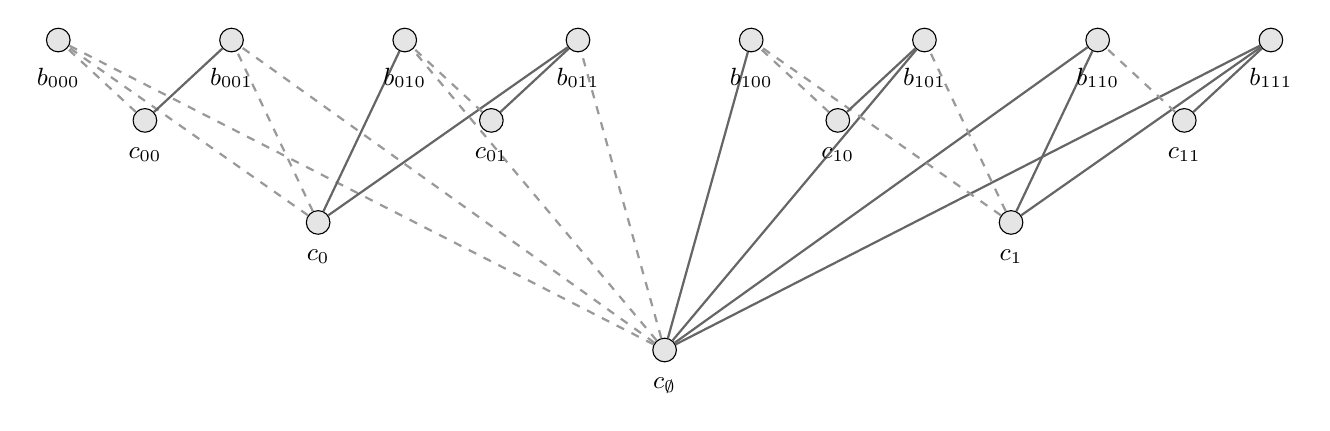
\begin{tikzpicture}[
        vertex/.style={circle, draw, fill=gray!20, minimum size=0.3cm, inner sep=1pt},
        label/.style={below=2pt, font=\small},
        solid edge/.style={draw, thick, black!60},
        dashed edge/.style={draw, dashed, thick, black!40},
    ]
	\node[vertex] (c_) at (8.8,0.0) {};
	\node[vertex] (c_0) at (4.4,1.62) {};
	\node[vertex] (c_1) at (13.200000000000001,1.62) {};
	\node[vertex] (c_00) at (2.2,2.9160000000000004) {};
	\node[vertex] (c_01) at (6.6000000000000005,2.9160000000000004) {};
	\node[vertex] (c_10) at (11.0,2.9160000000000004) {};
	\node[vertex] (c_11) at (15.400000000000002,2.9160000000000004) {};
	\node[vertex] (b_000) at (1.1,3.9366000000000008) {};
	\node[vertex] (b_001) at (3.3000000000000003,3.9366000000000008) {};
	\node[vertex] (b_010) at (5.5,3.9366000000000008) {};
	\node[vertex] (b_011) at (7.700000000000001,3.9366000000000008) {};
	\node[vertex] (b_100) at (9.9,3.9366000000000008) {};
	\node[vertex] (b_101) at (12.100000000000001,3.9366000000000008) {};
	\node[vertex] (b_110) at (14.3,3.9366000000000008) {};
	\node[vertex] (b_111) at (16.5,3.9366000000000008) {};
	\draw[dashed edge] (c_) -- (b_000);
	\draw[dashed edge] (c_) -- (b_001);
	\draw[dashed edge] (c_) -- (b_010);
	\draw[dashed edge] (c_) -- (b_011);
	\draw[solid edge] (c_) -- (b_100);
	\draw[solid edge] (c_) -- (b_101);
	\draw[solid edge] (c_) -- (b_110);
	\draw[solid edge] (c_) -- (b_111);
	\draw[dashed edge] (c_0) -- (b_000);
	\draw[dashed edge] (c_0) -- (b_001);
	\draw[solid edge] (c_0) -- (b_010);
	\draw[solid edge] (c_0) -- (b_011);
	\draw[dashed edge] (c_1) -- (b_100);
	\draw[dashed edge] (c_1) -- (b_101);
	\draw[solid edge] (c_1) -- (b_110);
	\draw[solid edge] (c_1) -- (b_111);
	\draw[dashed edge] (c_00) -- (b_000);
	\draw[solid edge] (c_00) -- (b_001);
	\draw[dashed edge] (c_01) -- (b_010);
	\draw[solid edge] (c_01) -- (b_011);
	\draw[dashed edge] (c_10) -- (b_100);
	\draw[solid edge] (c_10) -- (b_101);
	\draw[dashed edge] (c_11) -- (b_110);
	\draw[solid edge] (c_11) -- (b_111);
	\node[label] at (c_.south) {$c_{\emptyset}$};
	\node[label] at (c_0.south) {$c_{0}$};
	\node[label] at (c_1.south) {$c_{1}$};
	\node[label] at (c_00.south) {$c_{00}$};
	\node[label] at (c_01.south) {$c_{01}$};
	\node[label] at (c_10.south) {$c_{10}$};
	\node[label] at (c_11.south) {$c_{11}$};
	\node[label] at (b_000.south) {$b_{000}$};
	\node[label] at (b_001.south) {$b_{001}$};
	\node[label] at (b_010.south) {$b_{010}$};
	\node[label] at (b_011.south) {$b_{011}$};
	\node[label] at (b_100.south) {$b_{100}$};
	\node[label] at (b_101.south) {$b_{101}$};
	\node[label] at (b_110.south) {$b_{110}$};
	\node[label] at (b_111.south) {$b_{111}$};
    \end{tikzpicture}
    \caption{Example of a 3-tree. 
Notice that connections between disjoint sub-trees are not defined, and may be edges or non-edges in 
any combination.}
    \label{fig:k_tree}
\end{figure}


        Similarly to stability, we can define the \emph{tree bound} of a graph to measure the level of freeness from $k$-trees
        of graph.

        \begin{definition}[Definition 2.11 in~\cite{regularity_lemmas_for_stable_graphs}] \label{def:tree_bound}
            Suppose $G$ is a finite graph.
            We denote the \emph{tree bound} $k_{**} = k_{**}(G)$ as the minimal positive integer such that there is no
            $k_{**}$-tree $H = (\overline{c},\overline{b})$ in $G$.
        \end{definition}

        As mentioned earlier, the tree bound is closely related to the $k$-order property.
        The following theorem states that if a graph has a sufficiently large tree bound, then it has the $k$-order property
        and vice versa.

        \begin{theorem}[Lemma 6.7.9 in~\cite{model_theory}] \label{thm:tree_implies_order}
            If a graph $G$ has the $2^{k_{**}}$-order property, then the tree bound of $G$ is at least $k_{**} + 1$.
            On the other hand, if a graph $G$ has tree bound at least $k_{**} = 2^{k_*+1}-1$, then it has the $k_*$-order
            property.
            \begin{proof}
                For the first implication, just consider $\Partriangle{a_i \mid i \in \parcurly{1, \dots, 2^{k_{**}}-1}}$ and
                $\Partriangle{b_i \mid i \in \parcurly{0, \dots, 2^{k_{**}}-1}}$ to be the two sequences of vertices witnessing the
                $2^{k_{**}}$-order property in $G$, and thus for all $i,j \leq k$, $a_i R b_j$ if and only if $i \geq j$.
                It is straightforward to build a $k_{**}$-tree using these vertices.
                Take $\Partriangle{b_i \mid i \in \parcurly{0, \dots, 2^{k_{**}}-1}}$ to be the branches of the tree, indexing them by
                the binary decomposition of their index, and run the following construction for the nodes:
                \begin{itemize}
                    \item Initiate $C_\emptyset = \Partriangle{a_i \mid i \in \parcurly{0, \dots, 2^{k_{**}}-2}}$.
                    \item At each step $k \in \parcurly{0, k_{**}-1}$, for each $\eta \in \parcurly{0,1}^k$, take the middle
                        element of the sequence $C_\eta$ and set it to be the node $c_\eta$.
                        Then, the remaining first half of $C_\eta$ becomes the sequence $C_{\eta \frown \Partriangle{0}}$
                        and the second half is $C_{\eta \frown \Partriangle{1}}$.
                \end{itemize}
                Notice that at each step, the sequence $C_\eta$ has an odd number of elements.
                The resulting two sequences of nodes and branches form a $k_{**}$-tree.
                See \Cref{fig:half-graph_implies_k-tree} for a visual example of this construction.
                This finishes the argument for the first part of the argument.

                During the proof of the second implication, we say that a set of nodes $N$ of a $k$-tree
                $H = (\overline{c},\overline{b})$ \emph{contains} a $k'$-tree $H'$, if there exists a map
                $f \colon \parcurly{0,1}^{<k'} \longrightarrow \parcurly{0,1}^{<k}$ such that for all $\eta, \eta' \in \parcurly{0,1}^{<k'}$,
                $c_{f(\eta)}$ and $c_{f(\eta')}$ are in $N$, and if $\eta \frown \Partriangle{i} = \eta'$ then
                $f(\eta) \frown \Partriangle{i} \triangleleft f(\eta')$, for all $i \in \parcurly{0, 1}$.
                This clearly implies that there is a $k'$-tree $H'$ with nodes in $N$ and branches in $\overline{b}$.
                Simply, for each $\eta \in \parcurly{0,1}^{k'-1}$, pick exactly two branches $b_{\rho_0}$ and $b_{\rho_1}$ such that
                $f(\eta)\frown\Partriangle{i} \triangleleft \rho_i$ for $i \in \parcurly{0,1}$.

                Also, we will use $H'_i$ to denote the subtree of $H'$ consisting of the nodes $c_{f(\eta)}$ and branches
                $b_{f(\rho)}$ such that $\Partriangle{i} \triangleleft \eta$ and $\Partriangle{i} \triangleleft \rho$, with $\eta \in \parcurly{0,1}^{<k'}$
                and $\rho \in \parcurly{0,1}^{k'}$.
                Notice that, if $H$ is an $h$-tree, $H_0$ and $H_1$ are $(h-1)$-trees, and together with the root node
                singleton $\parcurly{c_{f(\emptyset)}}$, they partition $H$.

                Next, we prove the following claim, which shows that we can always find a tree
                in one of the parts of a bipartition of the nodes of a larger tree.

                \begin{claim} \label{clm:n_or_k_tree_in_partition_of_n_plus_k_tree}
                    For all $n, k \geq 0$, if $H$ is a $(n + k)$-tree and the nodes of $H$ are partitioned into two sets $N$ and $P$,
                    then either $N$ contains an $n$-tree or $P$ contains a $k$-tree.
                    \begin{proof}[Proof of \Cref{clm:n_or_k_tree_in_partition_of_n_plus_k_tree}]
                        We prove this by induction on $n + k$.
                        Clearly, the statement is true for the trivial case $n = k = 0$.
                        Suppose $n + k > 0$.
                        Without loss of generality, we may assume that the root node $c_\emptyset$ is in $N$.
                        Let $Z_i$ be the set of nodes of $H_i$, which is an $(n+k-1)$-tree.
                        By I.H., for each $i \in \parcurly{0,1}$, either $N \cap Z_i$ contains an $(n-1)$-tree or
                        $P \cap Z_i$ contains a $k$-tree.
                        If either $P \cap Z_0$ or $P \cap Z_1$ contains a $k$-tree, then $P$ contains a $k$-tree, and we are done.
                        Otherwise, both $N \cap Z_0$ and $N \cap Z_1$ contain an $(n-1)$-tree.
                        Since $c_\emptyset$ is in $N$, the root with the two $(k-1)$-tree are in $N$ and make an $n$-tree.
                        Thus, $N$ contains an $n$-tree.
                    \end{proof}
                \end{claim}

                \begin{figure}
    \centering

    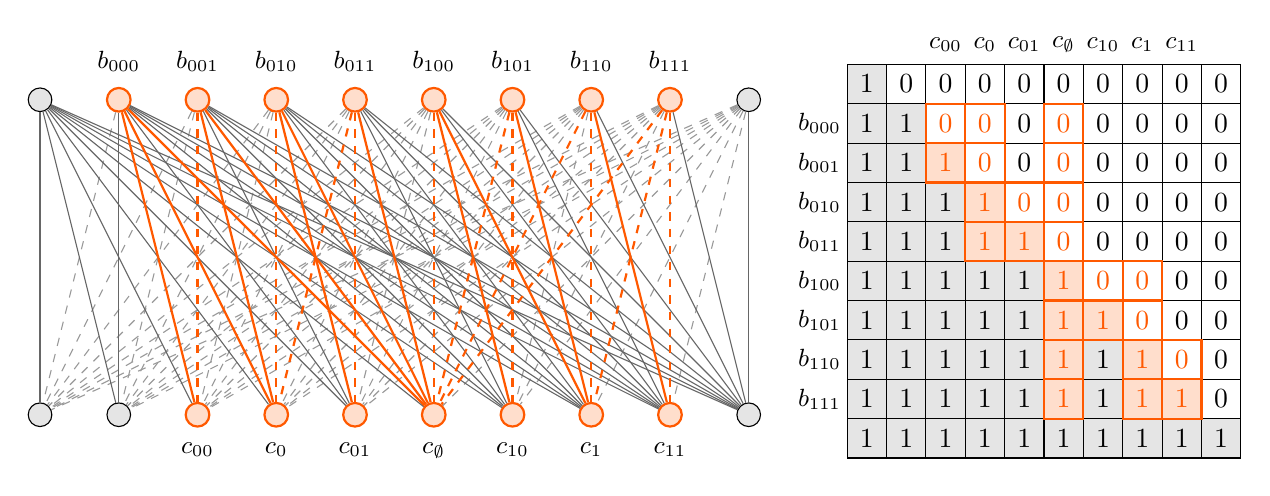
\begin{tikzpicture}[
        vertex/.style={circle, draw, fill=gray!20, minimum size=0.3 cm, inner sep=1pt},
        tree_vertex/.style={circle, thick, draw=orange!70!red, fill=orange!70!red!20, minimum size=0.3 cm, inner sep=1pt},
        label_a/.style={above=2pt, font=\small},
        label_b/.style={below=2pt, font=\small},
        node distance=1.5cm,
        solid edge/.style={draw, thick, black!60},
        dashed edge/.style={draw, dashed, thick, black!40},
        matrix cell/.style={draw, minimum size=0.5 cm, inner sep=0pt},
        matrix label/.style={font=\small, anchor=center}
    ]
	\node[vertex] (a_1) at (1,0) {};
	\node[tree_vertex] (a_2) at (2,0) {};
	\node[tree_vertex] (a_3) at (3,0) {};
	\node[tree_vertex] (a_4) at (4,0) {};
	\node[tree_vertex] (a_5) at (5,0) {};
	\node[tree_vertex] (a_6) at (6,0) {};
	\node[tree_vertex] (a_7) at (7,0) {};
	\node[tree_vertex] (a_8) at (8,0) {};
	\node[tree_vertex] (a_9) at (9,0) {};
	\node[vertex] (a_10) at (10,0) {};
	\node[vertex] (b_1) at (1,-4) {};
	\node[vertex] (b_2) at (2,-4) {};
	\node[tree_vertex] (b_3) at (3,-4) {};
	\node[tree_vertex] (b_4) at (4,-4) {};
	\node[tree_vertex] (b_5) at (5,-4) {};
	\node[tree_vertex] (b_6) at (6,-4) {};
	\node[tree_vertex] (b_7) at (7,-4) {};
	\node[tree_vertex] (b_8) at (8,-4) {};
	\node[tree_vertex] (b_9) at (9,-4) {};
	\node[vertex] (b_10) at (10,-4) {};
	\draw[solid edge, thin] (a_1) -- (b_1);
	\draw[dashed edge, thin] (a_2) -- (b_1);
	\draw[dashed edge, thin] (a_3) -- (b_1);
	\draw[dashed edge, thin] (a_4) -- (b_1);
	\draw[dashed edge, thin] (a_5) -- (b_1);
	\draw[dashed edge, thin] (a_6) -- (b_1);
	\draw[dashed edge, thin] (a_7) -- (b_1);
	\draw[dashed edge, thin] (a_8) -- (b_1);
	\draw[dashed edge, thin] (a_9) -- (b_1);
	\draw[dashed edge, thin] (a_10) -- (b_1);
	\draw[solid edge, thin] (a_1) -- (b_2);
	\draw[solid edge, thin] (a_2) -- (b_2);
	\draw[dashed edge, thin] (a_3) -- (b_2);
	\draw[dashed edge, thin] (a_4) -- (b_2);
	\draw[dashed edge, thin] (a_5) -- (b_2);
	\draw[dashed edge, thin] (a_6) -- (b_2);
	\draw[dashed edge, thin] (a_7) -- (b_2);
	\draw[dashed edge, thin] (a_8) -- (b_2);
	\draw[dashed edge, thin] (a_9) -- (b_2);
	\draw[dashed edge, thin] (a_10) -- (b_2);
	\draw[solid edge, thin] (a_1) -- (b_3);
	\draw[dashed edge, thin] (a_4) -- (b_3);
	\draw[dashed edge, thin] (a_5) -- (b_3);
	\draw[dashed edge, thin] (a_6) -- (b_3);
	\draw[dashed edge, thin] (a_7) -- (b_3);
	\draw[dashed edge, thin] (a_8) -- (b_3);
	\draw[dashed edge, thin] (a_9) -- (b_3);
	\draw[dashed edge, thin] (a_10) -- (b_3);
	\draw[solid edge, thin] (a_1) -- (b_4);
	\draw[dashed edge, thin] (a_6) -- (b_4);
	\draw[dashed edge, thin] (a_7) -- (b_4);
	\draw[dashed edge, thin] (a_8) -- (b_4);
	\draw[dashed edge, thin] (a_9) -- (b_4);
	\draw[dashed edge, thin] (a_10) -- (b_4);
	\draw[solid edge, thin] (a_1) -- (b_5);
	\draw[solid edge, thin] (a_2) -- (b_5);
	\draw[solid edge, thin] (a_3) -- (b_5);
	\draw[dashed edge, thin] (a_6) -- (b_5);
	\draw[dashed edge, thin] (a_7) -- (b_5);
	\draw[dashed edge, thin] (a_8) -- (b_5);
	\draw[dashed edge, thin] (a_9) -- (b_5);
	\draw[dashed edge, thin] (a_10) -- (b_5);
	\draw[solid edge, thin] (a_1) -- (b_6);
	\draw[dashed edge, thin] (a_10) -- (b_6);
	\draw[solid edge, thin] (a_1) -- (b_7);
	\draw[solid edge, thin] (a_2) -- (b_7);
	\draw[solid edge, thin] (a_3) -- (b_7);
	\draw[solid edge, thin] (a_4) -- (b_7);
	\draw[solid edge, thin] (a_5) -- (b_7);
	\draw[dashed edge, thin] (a_8) -- (b_7);
	\draw[dashed edge, thin] (a_9) -- (b_7);
	\draw[dashed edge, thin] (a_10) -- (b_7);
	\draw[solid edge, thin] (a_1) -- (b_8);
	\draw[solid edge, thin] (a_2) -- (b_8);
	\draw[solid edge, thin] (a_3) -- (b_8);
	\draw[solid edge, thin] (a_4) -- (b_8);
	\draw[solid edge, thin] (a_5) -- (b_8);
	\draw[dashed edge, thin] (a_10) -- (b_8);
	\draw[solid edge, thin] (a_1) -- (b_9);
	\draw[solid edge, thin] (a_2) -- (b_9);
	\draw[solid edge, thin] (a_3) -- (b_9);
	\draw[solid edge, thin] (a_4) -- (b_9);
	\draw[solid edge, thin] (a_5) -- (b_9);
	\draw[solid edge, thin] (a_6) -- (b_9);
	\draw[solid edge, thin] (a_7) -- (b_9);
	\draw[dashed edge, thin] (a_10) -- (b_9);
	\draw[solid edge, thin] (a_1) -- (b_10);
	\draw[solid edge, thin] (a_2) -- (b_10);
	\draw[solid edge, thin] (a_3) -- (b_10);
	\draw[solid edge, thin] (a_4) -- (b_10);
	\draw[solid edge, thin] (a_5) -- (b_10);
	\draw[solid edge, thin] (a_6) -- (b_10);
	\draw[solid edge, thin] (a_7) -- (b_10);
	\draw[solid edge, thin] (a_8) -- (b_10);
	\draw[solid edge, thin] (a_9) -- (b_10);
	\draw[solid edge, thin] (a_10) -- (b_10);
	\draw[solid edge, thick, orange!70!red] (a_2) -- (b_3);
	\draw[dashed edge, thick, orange!70!red] (a_3) -- (b_3);
	\draw[solid edge, thick, orange!70!red] (a_2) -- (b_4);
	\draw[solid edge, thick, orange!70!red] (a_3) -- (b_4);
	\draw[dashed edge, thick, orange!70!red] (a_4) -- (b_4);
	\draw[dashed edge, thick, orange!70!red] (a_5) -- (b_4);
	\draw[solid edge, thick, orange!70!red] (a_4) -- (b_5);
	\draw[dashed edge, thick, orange!70!red] (a_5) -- (b_5);
	\draw[solid edge, thick, orange!70!red] (a_2) -- (b_6);
	\draw[solid edge, thick, orange!70!red] (a_3) -- (b_6);
	\draw[solid edge, thick, orange!70!red] (a_4) -- (b_6);
	\draw[solid edge, thick, orange!70!red] (a_5) -- (b_6);
	\draw[dashed edge, thick, orange!70!red] (a_6) -- (b_6);
	\draw[dashed edge, thick, orange!70!red] (a_7) -- (b_6);
	\draw[dashed edge, thick, orange!70!red] (a_8) -- (b_6);
	\draw[dashed edge, thick, orange!70!red] (a_9) -- (b_6);
	\draw[solid edge, thick, orange!70!red] (a_6) -- (b_7);
	\draw[dashed edge, thick, orange!70!red] (a_7) -- (b_7);
	\draw[solid edge, thick, orange!70!red] (a_6) -- (b_8);
	\draw[solid edge, thick, orange!70!red] (a_7) -- (b_8);
	\draw[dashed edge, thick, orange!70!red] (a_8) -- (b_8);
	\draw[dashed edge, thick, orange!70!red] (a_9) -- (b_8);
	\draw[solid edge, thick, orange!70!red] (a_8) -- (b_9);
	\draw[dashed edge, thick, orange!70!red] (a_9) -- (b_9);
	\node[label_a] at (a_2.north) {$b_{000}$};
	\node[label_a] at (a_3.north) {$b_{001}$};
	\node[label_a] at (a_4.north) {$b_{010}$};
	\node[label_a] at (a_5.north) {$b_{011}$};
	\node[label_a] at (a_6.north) {$b_{100}$};
	\node[label_a] at (a_7.north) {$b_{101}$};
	\node[label_a] at (a_8.north) {$b_{110}$};
	\node[label_a] at (a_9.north) {$b_{111}$};
	\node[label_b] at (b_3.south) {$c_{00}$};
	\node[label_b] at (b_4.south) {$c_{0}$};
	\node[label_b] at (b_5.south) {$c_{01}$};
	\node[label_b] at (b_6.south) {$c_{\emptyset}$};
	\node[label_b] at (b_7.south) {$c_{10}$};
	\node[label_b] at (b_8.south) {$c_{1}$};
	\node[label_b] at (b_9.south) {$c_{11}$};

\begin{scope}[xshift=12 cm]
		\node[matrix cell, fill=gray!20] at (-0.5, 0.19999999999999996) {1};
		\node[matrix cell, fill=gray!20] at (-0.5, -0.30000000000000004) {1};
		\node[matrix cell, fill=gray!20] at (-0.5, -0.8) {1};
		\node[matrix cell, fill=gray!20] at (-0.5, -1.3) {1};
		\node[matrix cell, fill=gray!20] at (-0.5, -1.8) {1};
		\node[matrix cell, fill=gray!20] at (-0.5, -2.3) {1};
		\node[matrix cell, fill=gray!20] at (-0.5, -2.8) {1};
		\node[matrix cell, fill=gray!20] at (-0.5, -3.3) {1};
		\node[matrix cell, fill=gray!20] at (-0.5, -3.8) {1};
		\node[matrix cell, fill=gray!20] at (-0.5, -4.3) {1};
		\node[matrix cell] at (0.0, 0.19999999999999996) {0};
		\node[matrix cell, fill=gray!20] at (0.0, -0.30000000000000004) {1};
		\node[matrix cell, fill=gray!20] at (0.0, -0.8) {1};
		\node[matrix cell, fill=gray!20] at (0.0, -1.3) {1};
		\node[matrix cell, fill=gray!20] at (0.0, -1.8) {1};
		\node[matrix cell, fill=gray!20] at (0.0, -2.3) {1};
		\node[matrix cell, fill=gray!20] at (0.0, -2.8) {1};
		\node[matrix cell, fill=gray!20] at (0.0, -3.3) {1};
		\node[matrix cell, fill=gray!20] at (0.0, -3.8) {1};
		\node[matrix cell, fill=gray!20] at (0.0, -4.3) {1};
		\node[matrix cell] at (0.5, 0.19999999999999996) {0};
		\node[matrix cell, fill=gray!20] at (0.5, -1.3) {1};
		\node[matrix cell, fill=gray!20] at (0.5, -1.8) {1};
		\node[matrix cell, fill=gray!20] at (0.5, -2.3) {1};
		\node[matrix cell, fill=gray!20] at (0.5, -2.8) {1};
		\node[matrix cell, fill=gray!20] at (0.5, -3.3) {1};
		\node[matrix cell, fill=gray!20] at (0.5, -3.8) {1};
		\node[matrix cell, fill=gray!20] at (0.5, -4.3) {1};
		\node[matrix cell] at (1.0, 0.19999999999999996) {0};
		\node[matrix cell, fill=gray!20] at (1.0, -2.3) {1};
		\node[matrix cell, fill=gray!20] at (1.0, -2.8) {1};
		\node[matrix cell, fill=gray!20] at (1.0, -3.3) {1};
		\node[matrix cell, fill=gray!20] at (1.0, -3.8) {1};
		\node[matrix cell, fill=gray!20] at (1.0, -4.3) {1};
		\node[matrix cell] at (1.5, 0.19999999999999996) {0};
		\node[matrix cell] at (1.5, -0.30000000000000004) {0};
		\node[matrix cell] at (1.5, -0.8) {0};
		\node[matrix cell, fill=gray!20] at (1.5, -2.3) {1};
		\node[matrix cell, fill=gray!20] at (1.5, -2.8) {1};
		\node[matrix cell, fill=gray!20] at (1.5, -3.3) {1};
		\node[matrix cell, fill=gray!20] at (1.5, -3.8) {1};
		\node[matrix cell, fill=gray!20] at (1.5, -4.3) {1};
		\node[matrix cell] at (2.0, 0.19999999999999996) {0};
		\node[matrix cell, fill=gray!20] at (2.0, -4.3) {1};
		\node[matrix cell] at (2.5, 0.19999999999999996) {0};
		\node[matrix cell] at (2.5, -0.30000000000000004) {0};
		\node[matrix cell] at (2.5, -0.8) {0};
		\node[matrix cell] at (2.5, -1.3) {0};
		\node[matrix cell] at (2.5, -1.8) {0};
		\node[matrix cell, fill=gray!20] at (2.5, -3.3) {1};
		\node[matrix cell, fill=gray!20] at (2.5, -3.8) {1};
		\node[matrix cell, fill=gray!20] at (2.5, -4.3) {1};
		\node[matrix cell] at (3.0, 0.19999999999999996) {0};
		\node[matrix cell] at (3.0, -0.30000000000000004) {0};
		\node[matrix cell] at (3.0, -0.8) {0};
		\node[matrix cell] at (3.0, -1.3) {0};
		\node[matrix cell] at (3.0, -1.8) {0};
		\node[matrix cell, fill=gray!20] at (3.0, -4.3) {1};
		\node[matrix cell] at (3.5, 0.19999999999999996) {0};
		\node[matrix cell] at (3.5, -0.30000000000000004) {0};
		\node[matrix cell] at (3.5, -0.8) {0};
		\node[matrix cell] at (3.5, -1.3) {0};
		\node[matrix cell] at (3.5, -1.8) {0};
		\node[matrix cell] at (3.5, -2.3) {0};
		\node[matrix cell] at (3.5, -2.8) {0};
		\node[matrix cell, fill=gray!20] at (3.5, -4.3) {1};
		\node[matrix cell] at (4.0, 0.19999999999999996) {0};
		\node[matrix cell] at (4.0, -0.30000000000000004) {0};
		\node[matrix cell] at (4.0, -0.8) {0};
		\node[matrix cell] at (4.0, -1.3) {0};
		\node[matrix cell] at (4.0, -1.8) {0};
		\node[matrix cell] at (4.0, -2.3) {0};
		\node[matrix cell] at (4.0, -2.8) {0};
		\node[matrix cell] at (4.0, -3.3) {0};
		\node[matrix cell] at (4.0, -3.8) {0};
		\node[matrix cell, fill=gray!20] at (4.0, -4.3) {1};
		\node[matrix cell, thick, draw=orange!70!red, text=orange!70!red] at (0.5, -0.30000000000000004) {0};
		\node[matrix cell, thick, draw=orange!70!red, fill=orange!70!red!20, text=orange!70!red] at (0.5, -0.8) {1};
		\node[matrix cell, thick, draw=orange!70!red, text=orange!70!red] at (1.0, -0.30000000000000004) {0};
		\node[matrix cell, thick, draw=orange!70!red, text=orange!70!red] at (1.0, -0.8) {0};
		\node[matrix cell, thick, draw=orange!70!red, fill=orange!70!red!20, text=orange!70!red] at (1.0, -1.3) {1};
		\node[matrix cell, thick, draw=orange!70!red, fill=orange!70!red!20, text=orange!70!red] at (1.0, -1.8) {1};
		\node[matrix cell, thick, draw=orange!70!red, text=orange!70!red] at (1.5, -1.3) {0};
		\node[matrix cell, thick, draw=orange!70!red, fill=orange!70!red!20, text=orange!70!red] at (1.5, -1.8) {1};
		\node[matrix cell, thick, draw=orange!70!red, text=orange!70!red] at (2.0, -0.30000000000000004) {0};
		\node[matrix cell, thick, draw=orange!70!red, text=orange!70!red] at (2.0, -0.8) {0};
		\node[matrix cell, thick, draw=orange!70!red, text=orange!70!red] at (2.0, -1.3) {0};
		\node[matrix cell, thick, draw=orange!70!red, text=orange!70!red] at (2.0, -1.8) {0};
		\node[matrix cell, thick, draw=orange!70!red, fill=orange!70!red!20, text=orange!70!red] at (2.0, -2.3) {1};
		\node[matrix cell, thick, draw=orange!70!red, fill=orange!70!red!20, text=orange!70!red] at (2.0, -2.8) {1};
		\node[matrix cell, thick, draw=orange!70!red, fill=orange!70!red!20, text=orange!70!red] at (2.0, -3.3) {1};
		\node[matrix cell, thick, draw=orange!70!red, fill=orange!70!red!20, text=orange!70!red] at (2.0, -3.8) {1};
		\node[matrix cell, thick, draw=orange!70!red, text=orange!70!red] at (2.5, -2.3) {0};
		\node[matrix cell, thick, draw=orange!70!red, fill=orange!70!red!20, text=orange!70!red] at (2.5, -2.8) {1};
		\node[matrix cell, thick, draw=orange!70!red, text=orange!70!red] at (3.0, -2.3) {0};
		\node[matrix cell, thick, draw=orange!70!red, text=orange!70!red] at (3.0, -2.8) {0};
		\node[matrix cell, thick, draw=orange!70!red, fill=orange!70!red!20, text=orange!70!red] at (3.0, -3.3) {1};
		\node[matrix cell, thick, draw=orange!70!red, fill=orange!70!red!20, text=orange!70!red] at (3.0, -3.8) {1};
		\node[matrix cell, thick, draw=orange!70!red, text=orange!70!red] at (3.5, -3.3) {0};
		\node[matrix cell, thick, draw=orange!70!red, fill=orange!70!red!20, text=orange!70!red] at (3.5, -3.8) {1};
		\node[matrix label] at (-1.1, -0.30000000000000004) {$b_{000}$};
		\node[matrix label] at (0.5, 0.7) {$c_{00}$};
		\node[matrix label] at (-1.1, -0.8) {$b_{001}$};
		\node[matrix label] at (1.0, 0.7) {$c_{0}$};
		\node[matrix label] at (-1.1, -1.3) {$b_{010}$};
		\node[matrix label] at (1.5, 0.7) {$c_{01}$};
		\node[matrix label] at (-1.1, -1.8) {$b_{011}$};
		\node[matrix label] at (2.0, 0.7) {$c_{\emptyset}$};
		\node[matrix label] at (-1.1, -2.3) {$b_{100}$};
		\node[matrix label] at (2.5, 0.7) {$c_{10}$};
		\node[matrix label] at (-1.1, -2.8) {$b_{101}$};
		\node[matrix label] at (3.0, 0.7) {$c_{1}$};
		\node[matrix label] at (-1.1, -3.3) {$b_{110}$};
		\node[matrix label] at (3.5, 0.7) {$c_{11}$};
		\node[matrix label] at (-1.1, -3.8) {$b_{111}$};
   \end{scope}

    \end{tikzpicture}
    \caption{Example of a $3$-tree in a half-graph with 2 × 10 vertices. 
\emph{On the left}, solid lines show adjacent vertices, and dashed lines show non-adjacent vertices. 
Pairs of vertices without a line may or may not be connected. 
Orange lines and nodes highlight the $3$-tree structure. 
\emph{On the right} is the corresponding adjacency matrix. 
Again, orange cells highlight edges relative to the $3$-tree structure. }
    \label{fig:half-graph_implies_k-tree}
\end{figure}


                Suppose that $G$ has a tree bound of at least $2^{k_*+1}-1$, and thus contains a $(2^{k_*+1}-2)$-tree.
                We show by induction on $k_*-r$, with $1 \leq r \leq k_*$, that the following scenario $S_r$ holds.
                There are
                \begin{equation}\label{eq:tree_implies_order.1}
                    b_0, c_0, \dots, b_{q-1}, c_{q-1}, H, b_q, c_q, \dots, b_{k_*-r-1}, c_{k_*-r-1}
                \end{equation}
                such that:
                \begin{enumerate}
                    \item\label{itm:tree_implies_order.1} for all $i \in \parcurly{0, \dots, k_*-r-1}$, $b_i$ and $c_i$ are vertices in $G$,
                        and $H$ is a $(2^{r+1}-2)$-tree in $G$.
                    \item\label{itm:tree_implies_order.2} for all $i,j \in \parcurly{0, \dots, k_*-r-1}$, $b_i R c_j \Leftrightarrow i \geq j$.
                    \item\label{itm:tree_implies_order.3} if $c$ is a node of $H$, $b_i R c \Leftrightarrow i \geq q$.
                    \item\label{itm:tree_implies_order.4} if $b$ is a branch of $H$, $b R c_i \Leftrightarrow i < q$.
                \end{enumerate}

                The initial case $S_{k_*}$ only requires the existence of a $(2^{k_*+1}-2)$-tree in $G$, which is the premise.
                If the final case $S_1$ is true, then we are done:
                this case assumes that $H$ is a $2$-tree, hence there is a node $c_*$ and branch $b_*$ in $H$ that are adjacent.
                These vertices satisfy conditions \dref{itm:tree_implies_order.3} and \dref{itm:tree_implies_order.4}, so
                the sequence resulting from replacing $H$ in~\eqref{eq:tree_implies_order.1} by $b_*$, $c_*$ implies that $G$
                has the $k_*$-order property. \todo{specify k-order}

                To conclude the proof it remains to show that if $S_r$ holds, then so does $S_{r-1}$ for $r>1$.
                Assume $S_r$.
                Fixing $h = 2^r - 2$, by \dref{itm:tree_implies_order.1} we have that $H$ is a $(2h +2)$-tree.
                For each branch $b$ of $H$ we denote with $Z(b)$ the set of nodes $c$ of $H$ such that $b R c$.

                We have two cases:
                \begin{itemize}
                    \item \emph{Case 1.} There is a branch $b_*$ such that $Z(b_*)$ contains an $(h+1)$-tree $H'$.
                        In that case, we can take $c_*$ to be the top node of the $(h+1)$-tree, and $H_*$ to be the
                        $h$-subtree $H'_0$.
                        Replacing $H$ in~\eqref{eq:tree_implies_order.1} with $H_*$, $b_*$, $c_*$ in this order, the
                        conditions for $S_{r-1}$ are satisfied.
                    \item \emph{Case 2.} There is no branch $b$ such that $Z(b)$ contains an $(h+1)$-tree.
                        Now, let $c_*$ be the top node of $H$, $Z_1$ the set of nodes of $H_1$, and
                        $b_*$ any branch of $H_1$.
                        By the case assumption, $Z(b) \cap Z_1$ contains no $(h+1)$-tree, so by the claim
                        and the fact that $Z_1$ is the set of nodes of a $(2h+1)$-tree,
                        $Z_1 \setminus Z(b)$ contains an $h$-tree $H_*$.
                        Finally, replacing $H$ in~\eqref{eq:tree_implies_order.1} by $b_*$, $c_*$, $H_*$ in this order, the
                        conditions for $S_{r-1}$ are satisfied.
                \end{itemize}
                In any case, $S_{r-1}$ is satisfied, and the proof is complete.
            \end{proof}
        \end{theorem}

        \begin{remark}
            The key point of the proof of the second implication of \Cref{thm:tree_implies_order} is that the found
            bi-induced half-graph copy does not only utilize edges and non-edges of the $k$-tree structure itself.
            Instead, it relies on the fact that, for a tall enough tree, a $k$-order must appear in some way, leveraging
            some \say{unknown} edges, independently of disposition of the edges.
        \end{remark}

        The second implication of this theorem is of special interest in the next sections, as it proves that in the context
        of a $k$-stable graph no $2^{k+1}-2$-trees can be found.

        Given that the stability of the studied graphs is fixed for all proofs in the next sections, from now on we will use
        $k_*$ as the value of the non-$k$-property of the studied graphs, and $k_{**}$ for the associated tree bound.

\section{Section 4} \label{sec:section_4}

    This section works around the concept of \emph{$\epsilon$-indivisible} sets, a strong condition on the \regularity~of a subset
    respect to all the vertices of the graph.
    This condition results in pairs of sufficiently large subsets of vertices satisfying
    the \emph{average condition}, which (asymmetrically) strictly bounds the number of exceptional edges in the pair.
    Using these tools we obtain the first result in \Cref{lem:existance_of_ordered_f_indivisible_partitions_with_exceptions_bound},
    which proves the existence of a partition of highly \regular~pairs with no exceptions, at the cost of a
    non-homogeneous partition.
    Next, we improve the results obtaining an equitable partition in
    \Cref{thm:existance_of_equitative_partition_with_perfect_pairs_but_with_bound_exceptional_pairs}, but this time with a
    small number of exceptional pairs, and a tradeoff between a non-negligible remainder set and even smaller parts.
    The final result, \Cref{thm:equitative_partition_high_regularity_parts_grow_with_n}, achieves removing \irregular~pairs
    and reduce the size of the remainder set.
    All in all, even though the partitions of this section present a very strong form of \regularity, they all share
    the same drawback: a large number of parts that grows with the size of the graph, something that we will be dealing
    with in the next section.

    First step is defining \emph{indivisibility}.
    The general definition is for any function $f$, but for the rest of the section we are mostly interested in the case
    of $f(n) = n^\epsilon$, which we call $\epsilon$-indivisible, and at the end in the constant case $f(n) = c$.

    \begin{definition}[Definition 4.2(b)] \label{def:f_indivisible}
        Let $f: \mathbb{R} \longrightarrow \mathbb{R}$ be a function.
        We say that $A \subseteq G$ is \emph{$f$-indivisible} if for every $b \in G$,
        \[
            \parstraight{\overline{B}_{A,b}} < f(|A|)
        \]
    \end{definition}

    \begin{definition}[Definition 4.2(a)] \label{def:epsilon_indivisible}
        Let $\epsilon \in (0,1)$.
        We say that $A \subseteq G$ is \emph{$\epsilon$-indivisible} if for every $b \in G$,
        \[
            \parstraight{\overline{B}_{A,b}} < |A|^{\epsilon}
        \]
    \end{definition}

    \begin{remark}
        An $\epsilon$-indivisible set is $f$-indivisible for $f(n) = n^\epsilon$.
    \end{remark} \todo{Redundant.}

    A natural follow-up question, is how strongly bounded are exceptions in the context of two indivisible sets.
    The following lemma measures precisely that, although doing so in asymmetrically.

    \begin{lemma}[Claim 4.6)] \label{lem:average_condition_statement}
        Let $G$ be a finite graph.
        Suppose $A, B \subseteq G$ such that $A$ is $f$-indivisible, $B$ is $g$-indivisible, and $f(|A|) g(|B|) < \frac{1}{2} |B|$.
        Then, the truth value $t = t(A,B)$ satisfies that for all but $< f(|A|)$ of the $a \in A$ for all but $< g(|B|)$ of
        the $b \in B$ we have that $a R b \equiv t$.
        \begin{proof}
            Since $B$ is $g$-indivisible, for each $a \in A$ we have that $\parstraight{\overline{B}_{B,a}} < g(|B|)$.
            Let $U_i = \parcurly{a \in A \mid t(a,B) \equiv i}$ for $i \in \parcurly{0,1}$.
            If either $U_i$ satisfies $|U_i| < f(|A|)$ then the statement is true.
            Suppose not.
            Then, there are $W_i \subseteq U_i$ with $|W_i| = f(|A|)$ for $i \in \parcurly{0,1}$.
            Now, let $V = \parcurly{b \in B \mid (\exists a \in W_0 \mid a R b) \vee (\exists a \in W_1 \mid \lnot a R b)}$,
            i.e. the $b$'s which are an exception for some $a \in W_0 \cup W_1$.
            Then, $|V| < |W_0| g(|B|) + |W_1| g(|B|) = 2 f(|A|) g(|B|) < |B|$, where the first inequality follows the
            $g$-indivisibility of $B$.
            Finally, there is a $b_* \in B \setminus V$ such that $\forall a \in W_0$ $\lnot a R b_*$ and
            $\forall a \in W_1$ $a R b_*$ with $|W_0| = |W_1| = f(|A|)$, which contradicts the $f$-indivisibility of $A$.
        \end{proof}
    \end{lemma}

    \begin{definition}
        We say that the pair $(A,B)$ with $A$ $f$-indivisible and $B$ $g$-indivisible satisfies the \emph{average condition} if
        $f(|A|) g(|B|) < \frac{1}{2} |B|$ and thus the statement of \Cref{lem:average_condition_statement} is true for
        the pair $(A,B)$.
    \end{definition}

    \begin{remark}
        The condition $f(|A|) g(|B|) < \frac{1}{2} |B|$ makes ordering of the pair $(A,B)$ matter, that is,
        \[
            (A,B) \text{ has the average condition } \not\Rightarrow (B,A) \text{ has the average condition }
        \]
    \end{remark}

    \begin{remark}[Remark 4.7]
        When $f(n) = n^\epsilon$ and $g(n) = n^\zeta$, the average condition is $|A|^\epsilon |B|^\zeta < \frac{1}{2} |B|$.
    \end{remark}
    \todo{I don't think this is useful in any way.}

    Next, we are interested in studying how the average condition of an indivisible pair controls the homogeneity
    \todo{Define homogeneity.}
    of large enough subpairs, in the sense of bounding exceptional edges.
    We study the $f$ and $\epsilon$ case separately, as the specific case of $\epsilon$ gives a slightly better condition
    on the range of the size of the subpair.

    \begin{lemma}[Claim 4.8] \label{lem:exceptions_bound_of_epsilon_indivisible_sets}
        Let $A$ be $\epsilon$-indivisible, $B$ $\zeta$-indivisible and let the pair $(A,B)$ satisfy the average condition.
        Then, for all $\epsilon_1 \in \parround{0, 1-\epsilon}$, $\zeta_1 \in \parround{0, 1-\zeta}$, $A' \subseteq A$
            and $B' \subseteq B$ such that $|A'| \geq |A|^{\epsilon + \epsilon_1}$ and $|B'| \geq |B|^{\zeta + \zeta_1}$,
            we have that:
        \[
            \frac{|\parcurly{(a,b) \in (A',B') \mid a R b \equiv \neg t(A,B)}|}{|A' \times B'|} \leq
                \frac{1}{|A|^{\epsilon_1}} + \frac{1}{|B|^{\zeta_1}}
        \]
        \begin{proof}
            Notice:
            \begin{itemize}
                \item There are at most $|A|^\epsilon$ vertices of $A$ (hence in $A' \subseteq A$) which are exceptional
                    (in the sense of the average condition).
                \todo{This is not the same use of the word exceptional as defined in \Cref{sec:section_3}.}
                \item For each $a \in A$ (hence in $A' \subseteq A$) not exceptional, there are at most $|B|^\zeta$ elements
                    $b \in B$ such that $(a,b)$ does not satisfy the truth value $t(A,B)$, i.e. that are exceptional.
            \end{itemize}
            Putting it all together:
            \todo{This makes my eyes bleed.}
            \[
                \begin{split}
                    \frac{|\parcurly{(a,b) \in (A',B') \mid a R b \equiv \neg t(A,B)}|}{|A' \times B'|}
                        &\leq \frac{|A|^\epsilon |B'| + (|A'| - |A|^\epsilon) |B|^\zeta}{|A'| |B'|} \\
                        &= \frac{|A|^\epsilon}{|A'|} + \frac{|A'| - |A|^\epsilon}{|A'|} \frac{|B|^\zeta}{|B'|} \\
                        &\leq \frac{|A|^\epsilon}{|A'|} + \frac{|B|^\zeta}{|B'|} \\
                        &\leq \frac{|A|^\epsilon}{|A|^{\epsilon + \epsilon_1}} + \frac{|B|^\zeta}{|B|^{\zeta + \zeta_1}} \\
                        &= \frac{1}{|A|^{\epsilon_1}} + \frac{1}{|B|^{\zeta_1}}
                \end{split}
            \]
        \end{proof}
    \end{lemma}

    \todo{This next generalization may seem to make previous lemma redundant. But they actually prove different results.
        But is it worth to keep both?}

    \begin{lemma}[$f$-indivisible version] \label{lem:exceptions_bound_of_f_indivisible_sets}
        Let $A$ be $f$-indivisible, $B$ $g$-indivisible and let the pair $(A,B)$ satisfy the average condition.
        Then, for all $\epsilon_1 \in \parround{0, 1-\frac{f(|A|)}{|A|}}$, $\zeta_1 \in \parround{0, 1-\frac{g(|B|)}{|B|}}$, $A' \subseteq A$
            and $B' \subseteq B$ such that $|A'| \geq f(|A|) |A|^{\epsilon_1}$ and $|B'| \geq g(|B|) |B|^{\zeta_1}$,
            we have that:
        \[
            \frac{|\parcurly{(a,b) \in (A',B') \mid a R b \equiv \neg t(A,B)}|}{|A' \times B'|} \leq
                \frac{1}{|A|^{\epsilon_1}} + \frac{1}{|B|^{\zeta_1}}
        \]
        \begin{proof}
            Notice:
            \begin{itemize}
                \item There are at most $f(|A|)$ elements of $A$ (hence in $A' \subseteq A$) which are exceptional
                    (in the sense of the average condition).
                \item For each $a \in A$ (hence in $A' \subseteq A$) not exceptional, there are at most $g(|B|)$ elements
                    $b \in B$ such that $(a,b)$ does not satisfy the truth value $t(A,B)$, i.e. that are exceptional.
            \end{itemize}
            Putting it all together:
            \[
                \begin{split}
                    \frac{|\parcurly{(a,b) \in (A',B') \mid a R b \equiv \neg t(A,B)}|}{|A' \times B'|}
                        &\leq \frac{f(|A|) |B'| + (|A'| - f(|A|)) g(|B|)}{|A'| |B'|} \\
                        &= \frac{f(|A|)}{|A'|} + \frac{|A'| - f(|A|)}{|A'|} \frac{g(|B|)}{|B'|} \\
                        &\leq \frac{f(|A|)}{|A'|} + \frac{g(|B|)}{|B'|} \\
                        &\leq \frac{f(|A|)}{f(|A|) |A|^{\epsilon_1}} + \frac{g(|B|)}{g(|B|) |B|^{\zeta_1}} \\
                        &= \frac{1}{|A|^{\epsilon_1}} + \frac{1}{|B|^{\zeta_1}}
                \end{split}
            \]
        \end{proof}
    \end{lemma}

    For later use, we are particularly interested in the case when $f(n) = c$.
    \todo{This may be skipped, and be directly commented in the appropiate remark following the theorem.}

    \begin{corollary}[Corollary 4.9]
        Let $A$ and $B$ be $f$-indivisible with $f(n) = c$ and $(A,B)$ satisfy the average condition.
        Then, for all $\epsilon_1 \in (0, 1 - \frac{c}{|A|})$, $\zeta_1 \in (0, 1 - \frac{c}{|B|})$, $A' \subseteq A$ and
            $B' \subseteq B$ with $|A'| \geq c |A|^{\epsilon_1}$ and $|B'| \geq c |B|^{\zeta_1}$, we have:
        \[
            \frac{|\parcurly{(a,b) \in (A',B') \mid a R b \equiv \neg t(A,B)}|}{|A' \times B'|} \leq
                \frac{1}{|A|^{\epsilon_1}} + \frac{1}{|B|^{\zeta_1}}
        \]
        \begin{proof}
            Use \Cref{lem:exceptions_bound_of_f_indivisible_sets} with $f(n) = c$.
        \end{proof}
    \end{corollary}

    \begin{remark}\label{rmk:sufficient_requirement_for_average_condition}
        Notice that the average condition is easily satisfied if the pair satisfies a condition on the size of its sets.
        If $f(n) = n^\epsilon$, $A$ and $B$ are $f$-indivisible, and $\parstraight{B} \geq \parstraight{A} \geq m$,
        then $m^{1-2\epsilon} > 2$ is sufficient for the average condition to hold for the pair $(A,B)$:
        \[
            \frac{|A|^\epsilon |B|^\epsilon}{|B|}
                \leq \frac{|B|^{2\epsilon}}{|B|}
                = \frac{1}{|B|^{1-2\epsilon}}
                = \frac{1}{m^{1-2\epsilon}}
                < \frac{1}{2}
        \]
        We will be using this fact in the context of a sequence of non-zero natural numbers
        $\parcurly{m_\ell \mid \ell \in \parcurly{0, \dots, k_{**}}}$ where $\floor{m_\ell^\epsilon} = m_{\ell+1}$
        for some $\epsilon \in (0, \frac{1}{2})$ and for all $\ell \in \parcurly{0, \dots, k_{**}-1}$.
        Here, $2 < (m_{k_{**}-1})^{1-2\epsilon}$ is sufficient for any $f$-indivisible $A$ and $B$, with
        $|A|, |B| \in \parcurly{m_0, \dots, m_{k_{**}-1}}$, to satisfy the average condition.
    \end{remark}

    Now that we have proven some properties of indivisible sets, we are actually interested in whether they can be
    found in a graph.
    It turns out that the non-$k$-order property, or more specifically the associated tree bound, is sufficient for
    proving it.
    The proof resumes in assuming that there is no indivisible set to recursively refine a \say{semi-partition}
    \todo{Lluis: hi ha alguna manera de dir una partició que no cubreix tots els vertex amb una paraula?}
    which by construction contains a $k_{**}$-tree.

    \begin{lemma}[Claim 4.3] \label{lem:existance_of_indivisible_sets}
        Let $G$ be a finite graph with the non-$k_*$-property and $f: \mathbb{R} \longrightarrow \mathbb{R}$ a function
        such that $x \geq f(x)$.
        Let $\parcurly{m_\ell \mid \ell \in \parcurly{0, \dots, k_{**}}}$ be a sequence of non-zero natural numbers such that
        for all $\ell \in \parcurly{0, \dots, k_{**}-1}$, $f(m_{\ell}) \geq m_{\ell+1}$.
        If $A \subseteq G$, $|A| \geq m_0$, then for some $\ell \in \parcurly{0, \dots, k_{**}-1}$ there is a subset $B \subseteq A$
        of size $m_\ell$ which is $f$-indivisible.
        % It may seem that m_{k_{**}} has no use, but it actually ensures that the smallest A_\eta is not empty.
        \begin{proof}
            Suppose not.
            Then we can construct the sequences $\Partriangle{b_\eta \mid \eta \in \parcurly{0,1}^{<k}}$ and $\Partriangle{A_\eta \mid \eta \in \parcurly{0,1}^{\leq k}}$
            on induction over $k = |\eta|$, satisfying:
            \begin{enumerate}
                \item\label{itm:existance_of_indivisible_sets.1} $A_{\eta^\frown \Partriangle{i}} \subseteq A_{\eta}$, $\forall i \in \parcurly{0,1}$, $\forall k \in \parcurly{0, \dots, k_{**}-1}$
                \item\label{itm:existance_of_indivisible_sets.2} $A_{\eta^\frown \Partriangle{0}} \cap A_{\eta^\frown \Partriangle{1}} = \emptyset$, $\forall k \in \parcurly{0, \dots, k_{**}-1}$
                \item\label{itm:existance_of_indivisible_sets.3} $|A_\eta| = m_k$, $\forall k \in \parcurly{0, \dots, k_{**}}$
                \item\label{itm:existance_of_indivisible_sets.4} $b_\eta \in G$ witnessing that $A_\eta$ is not $f$-indivisible, $\forall k \in \parcurly{0, \dots, k_{**}-1}$
                \item\label{itm:existance_of_indivisible_sets.5} $A_{\eta^\frown \Partriangle{i}} \subseteq A_\eta^{(i)} = \parcurly{a \in A_\eta \mid a R b_\eta \equiv (i=1)}$,
                    $\forall \in \parcurly{0,1}$, $\forall k \in \parcurly{0, \dots, k_{**}-1}$
            \end{enumerate}
            Let's prove the induction.
            For $k=0$, consider any $A_{\Partriangle{\cdot}} \subseteq A$, satisfying $|A_{\Partriangle{\cdot}}| = m_0$, and
            any $b_{\Partriangle{\cdot}}$ witnessing the non-$f$-indivisibility of $A_{\Partriangle{\cdot}}$.
            For $k > 0$ we can assume by hypothesis that $A_\eta$, with $|A_\eta| = m_{k}$, is not $f$-indivisible.
            Thus, there exists $b_\eta$ such that $A_\eta^{(i)} \geq f(m_{k}) \geq m_{k+1}$ (\dref{itm:existance_of_indivisible_sets.4}), and we can choose
            $A_{\eta^\frown \Partriangle{i}} \subseteq A_\eta^{(i)}$ (\dref{itm:existance_of_indivisible_sets.5}), such that
            $|A_{\eta^\frown \Partriangle{i}}| = m_{k+1}$ $\forall i \in \parcurly{0,1}$ (\dref{itm:existance_of_indivisible_sets.3}).
            \dref{itm:existance_of_indivisible_sets.1} and \dref{itm:existance_of_indivisible_sets.2} are satisfied by the definition of $A_\eta^{(i)}$.
            Now, for all $\eta$ such that $|\eta| = k_{**}$, consider some element $a_\eta \in A_\eta$, which exists since $m_\ell > 0$
            for all $\ell$.
            Then, we have two sequences $\Partriangle{b_\eta \mid \eta \in \parcurly{0,1}^{<k_{**}}}$ and $\Partriangle{a_\eta \mid \eta \in \parcurly{0,1}^{k_{**}}}$
            satisfying the $k_{**}$-tree property: for all $\rho \in \parcurly{0,1}^{<k_{**}}$ and $\eta \in \parcurly{0,1}^{k_{**}}$
            if given $\ell \in \parcurly{0, 1}$ we have $\rho^\frown \Partriangle{\ell} \trianglelefteq \eta$ then
            $(a_\eta R b_\rho) \equiv \parround{\ell = 1}$ since $a_\eta \in A_\eta \subseteq A_{\rho ^\frown \Partriangle{i}}$.
            This contradicts the $k_{**}$ tree bound.
        \end{proof}
    \end{lemma}

    The previous proof can be iteratively used to partition the graph into indivisible parts, with a small reminder.
    As the average condition cares about the ordering, we define the partition as a tuple instead of a family of sets,
    and fix an ascending order on the size of the parts.

    \begin{lemma}[Claim 4.4 + 4.5] \label{lem:existance_of_ordered_f_indivisible_partitions}
        Let $G$ be a finite graph with the non-$k_{*}$-order property and $f: \mathbb{R} \longrightarrow \mathbb{R}$ a function
        such that $x \geq f(x)$.
        Let $\parcurly{m_\ell \mid \ell \in \parcurly{0, \dots, k_{**}}}$ be a sequence of non-zero natural numbers such that
        for all $\ell \in \parcurly{0, \dots, k_{**}-1}$, $f(m_{\ell}) \geq m_{\ell+1}$.
        If $A \subseteq G$ with $|A| = n$, then we can find a sequence $\overline{A} = \Partriangle{A_j \mid j \in \parcurly{1, \dots, j(*)}}$
        and reminder $B = A \setminus \bigcup \overline{A}$ such that:
        \begin{enumerate}
            \item \label{itm:existance_of_ordered_f_indivisible_partitions.1} For each $j \in \parcurly{1, \dots, j(*)}$, $A_j$ is $f$-indivisible.
            \item \label{itm:existance_of_ordered_f_indivisible_partitions.2} For each $j \in \parcurly{1, \dots, j(*)}$, $|A_j| \in \parcurly{m_0, \dots, m_{k_{**}-1}}$.
            \item \label{itm:existance_of_ordered_f_indivisible_partitions.3} $A_j \subseteq A \setminus \bigcup\parcurly{A_i \mid i < j}$, in particular $A_i \cap A_j = \emptyset$ $\forall i \neq j$.
            \item \label{itm:existance_of_ordered_f_indivisible_partitions.4} $|B| < m_0$.
            \item \label{itm:existance_of_ordered_f_indivisible_partitions.5} $\overline{A}$ is $\leq$-increasing.
        \end{enumerate}
        \begin{proof}
            Iteratively, apply \Cref{lem:existance_of_indivisible_sets} to the remainder $A \setminus \bigcup \parcurly{A_i \mid i < j}$
            (\dref{itm:existance_of_ordered_f_indivisible_partitions.3}) to get an $f$-indivisible $A_j$ (\dref{itm:existance_of_ordered_f_indivisible_partitions.1}) of size $m_\ell$, $\ell \in \parcurly{0, \dots, k_{**}-1}$
            (\dref{itm:existance_of_ordered_f_indivisible_partitions.2}) until less then $m_0$ vertices are available (\dref{itm:existance_of_ordered_f_indivisible_partitions.4}).
            To conclude, reorder the indices of the $A_j$'s in ascending size order (\dref{itm:existance_of_ordered_f_indivisible_partitions.5}).
        \end{proof}
    \end{lemma}

    Finally, we ensure the pairs satisfy the average condition by simply requiring a minimal size of the parts,
    a condition that can be easily integrated in the definition of the sequence of integers.

    \begin{lemma}[Claim 4.10] \label{lem:existance_of_ordered_f_indivisible_partitions_with_exceptions_bound}
        Let $G$ be a finite graph with the non-$k_{*}$-order property.
        Let $\parcurly{m_\ell \mid \ell \in \parcurly{0, \dots, k_{**}}}$ be a sequence of non-zero natural numbers such that
        $n \geq m_0$ and for all $\ell \in \parcurly{0, \dots, k_{**}-1}$, $\floor{m_\ell^\epsilon} = m_{\ell+1}$,
        for some $\epsilon \in (0, \frac{1}{2})$ such that $2 < (m_{k_{**}-1})^{1-2\epsilon}$.
        \todo{Last condition can be changed (and probably should) for a condition on $m_{k_{**}}$}
        If $A \subseteq G$ with $|A| = n$, then we can find a sequence $\overline{A} = \Partriangle{A_i \mid i \in \parcurly{1, \dots, i(*)}}$
        and reminder $B = A \setminus \bigcup \overline{A}$ satisfying:
        \begin{enumerate}
            \item \label{itm:existance_of_ordered_f_indivisible_partitions_with_exceptions_bound.1} For each $i \in \parcurly{1, \dots, i(*)}$, $A_i$ is $\epsilon$-indivisible.
            \item \label{itm:existance_of_ordered_f_indivisible_partitions_with_exceptions_bound.2} For each $i \in \parcurly{1, \dots, i(*)}$, $|A_i| \in \parcurly{m_0, \dots, m_{k_{**}-1}}$.
            \item \label{itm:existance_of_ordered_f_indivisible_partitions_with_exceptions_bound.3} $A_i \cap A_j = \emptyset$ for all $i \neq j$.
            \item \label{itm:existance_of_ordered_f_indivisible_partitions_with_exceptions_bound.4} $|B| < m_0$.
            \item \label{itm:existance_of_ordered_f_indivisible_partitions_with_exceptions_bound.5} $\overline{A}$ is $\leq$-increasing.
            \item \label{itm:existance_of_ordered_f_indivisible_partitions_with_exceptions_bound.6} If $\zeta \in \parround{0,\epsilon^{k_{**}}}$ then for every $i,j \in \parcurly{1, \dots, i(*)}$ with $i < j$,
                $A \subseteq A_i$ ad $B \subseteq A_j$ such that $|A| \geq |A_i|^{\epsilon + \zeta}$ and $|B| \geq |A_j|^{\epsilon + \zeta}$
                we have that:
                \[
                    \begin{split}
                        \frac{|\parcurly{(a,b) \in (A,B) \mid a R b \equiv \neg t(A_i,A_j)}|}{|A \times B|}
                            &\leq \frac{1}{|A_i|^\zeta} + \frac{1}{|A_j|^\zeta} \\
                            &\leq \frac{1}{|A|^\zeta} + \frac{1}{|B|^\zeta}
                    \end{split}
                \]
        \end{enumerate}
        \begin{proof}
            The five points are direct consequence of \Cref{lem:existance_of_ordered_f_indivisible_partitions},
            setting $f(x) = x^\epsilon$.
            Now, by \dref{itm:existance_of_ordered_f_indivisible_partitions_with_exceptions_bound.2}, for any $A_i, A_j \in \overline{A}$ with $i < j$
            there is some $\ell \in \parcurly{0, \dots, k_{**}-1}$ such that $|A_i| \leq |A_j| = m_\ell$.
            Also, it follows the condition $2 < (m_{k_{**}-1})^{1-2\epsilon}$ and \Cref{rmk:sufficient_requirement_for_average_condition}
            that the pair $(A_i,A_j)$ satisfies the average condition.
            Finally, notice that $\epsilon^{k_{**}} < \epsilon < 1 - \epsilon$ since $\epsilon \in (0, \frac{1}{2})$,
            so that $\zeta \in (0, \epsilon ^ {k_{**}}) \subseteq (0, 1 - \epsilon)$ and the condition for
            \Cref{lem:exceptions_bound_of_epsilon_indivisible_sets} is satisfied.
            This gives us \dref{itm:existance_of_ordered_f_indivisible_partitions_with_exceptions_bound.6} and concludes the proof of the statement.
        \end{proof}
    \end{lemma}
    \todo{Maybe merge the last two lemmas?}

    \begin{remark}
        For sufficiently small $\epsilon$, the condition $2 < (m_{k_{**}-1})^{1-2\epsilon}$ is almost, trivial.
        For example, if $\epsilon < \frac{1}{4}$, then we are just requiring that $m_{k_{**}-1} \geq 4$.
    \end{remark}

    As stated earlier, the principal drawback of the previous result is that the obtained partition is not equitable.
    To deal with this, we study the event of randomly partitioning a pair of indivisible sets
    \todo{Hehe, "partition indivisible sets", sona contradictiu.}
    into subparts of equal size.
    We prove that the event of a pair of subparts of the refinement being either fully connected or completely empty,
    is satisfied with very high probability.

    \begin{definition}
        Let $A, B$ be $f$-indivisible sets with $f(A) f(B) < \frac{1}{2} |B|$.
        Let $\Partriangle{A_i \mid i \in \parcurly{1, \dots, i_A}}$ be a partition of $A$ with $|A_i| = m$ for all
        $i \in \parcurly{1, \dots, i_A}$ and $\Partriangle{B_i \mid i \in \parcurly{1, \dots, i_B}}$ be a partition of
        $B$ with $|B_i| = m$ for all $i \in \parcurly{1, \dots, i_B}$.
        We define $\varepsilon^+_{A_i,A_j,m}$ as the event:
        \[
            \forall a \in A_i \ \forall b \in B_i, a R b = t(A,B)
        \]
    \end{definition}

    \begin{lemma}[Claim 4.13] \label{lem:bound_on_the_probability_of_a_subpair_having_no_exceptions}
        Let $G$ be a finite graph with the non-$k_{*}$-order property.
        Let $\Partriangle{m_\ell \mid \ell \in \parcurly{0, \dots, k_{**}}}$ be a sequence of non-zero natural numbers such that
        $n \geq m_0 \geq n^\epsilon$ \todo{Should be mentioned that this is a strong limitation which is not mentioned in the original
        paper, but required for the calculations (sin hacer trampa).} and for all $\ell \in \parcurly{0, \dots, k_{**}-1}$, $m_\ell^\epsilon = m_{\ell+1}$,
        \todo{Here we have enforced the equality. Should be commented that this is easily achievable as we do in the next results.}
        for some $\epsilon \in (0, \frac{1}{2})$ such that $2 < (m_{k_{**}-1})^{1-2\epsilon}$.
        Let $A_1, A_2 \subseteq G$ be two $\epsilon$-indivisible subsets such that $|A_1| = m_{\ell_1}$ and $|A_2| = m_{\ell_2}$
        for some $\ell_1, \ell_2 \in \parcurly{0, \dots, k_{**}-1}$ and $|A_1| \leq |A_2|$.
        Let $c \in (0, 1-\epsilon)$ and $\zeta \leq \frac{1 - \epsilon - c}{3}\epsilon^{k_{**}}$ such that
        $m \coloneqq n^\zeta$ divides $|A_1|$ and $|A_2|$.
        Then, let $\Partriangle{A_{1,s} \mid s \in \bparcurly{1, \dots, \frac{|A_1|}{m}}}$ and
        $\Partriangle{A_{2,t} \mid t \in \bparcurly{1, \dots, \frac{|A_2|}{m}}}$ be random partitions of $A_1$ and $A_2$
        respectively, with pieces of size $m$.
        We have that
        \[
            P(\varepsilon^+_{A_{1,s},A_{2,t},m}) \geq 1 - \frac{2}{n^{c\epsilon^{k_{**}}}}
        \]
        \begin{proof}
            Fix $s \in \frac{|A_1|}{m}$, $t \in \frac{|A_2|}{m}$.
            It follows from the condition $2 < (m_{k_{**}-1})^{1-2\epsilon}$ and \Cref{rmk:sufficient_requirement_for_average_condition}
            that the pair $(A_{1}, A_{2})$ satisfies the average condition.
            Let $U_1 = \bparcurly{a \in A_1 \mid \bparstraight{\parcurly{b \in A_2 \mid a R b \equiv \neg t(A_1, A_2)}} \geq |A_2|^\epsilon}$
            and for each $a \in A_1 \setminus U_1$ let $U_{2,a} = \parcurly{b \in A_j \mid a R b \equiv \neg t(A_1, A_2)}$.
            By \Cref{lem:average_condition_statement}, $|U_1| \leq |A_1|^\epsilon$ and $\forall a \in A_1 \setminus U_1$,
            $|U_{2,a}| \leq |A_2|^\epsilon$.
            Now, given $\bparcurly{1, \dots, \frac{|A_1|}{m}}$, we can bound the probability $P_1$ that
            $A_{1,s} \cap U_1 \neq \emptyset$ as follows:
            \[
                \begin{split}
                    P_1
                        & \leq \frac{|U_1|}{|A_1|} + \dots + \frac{|U_1|}{|A_1|-m+1}
                            < \frac{m |U_1|}{|A_1| - m}
                            \leq \frac{m |A_1|^\epsilon}{|A_1| - m} \\
                        & \leq \frac{m^2 |A_1|^\epsilon}{|A_1|}
                            = \frac{m^2}{|A_1|^{1-\epsilon}}
                            = \frac{m^2}{m_0^{\parround{1-\epsilon} \epsilon^{\ell_1}}} % the requirement of equality in the condition of m_l's is required here
                            \leq \frac{n^{2 \zeta}}{n^{(1-\epsilon)\epsilon^{\ell_1 + 1}}} \\
                        & \leq \frac{n^{2\frac{1-\epsilon-c}{3} \epsilon^{k_{**}}}}{n^{(1-\epsilon)\epsilon^{k_{**}}}}
                            \leq \frac{n^{(1-\epsilon-c) \epsilon^{k_{**}}}}{n^{(1-\epsilon)\epsilon^{k_{**}}}}
                            = \frac{1}{n^{c \epsilon^{k_{**}}}}
                \end{split}
            \]
            The forth inequality comes from the fact that $\frac{(|A_i| - m) m}{|A_i|} \geq 1$.
            Then, if $A_{1,s} \cap U_1= \emptyset$, we have that $|\bigcup_{a \in A_{1,s}} U_{2,a}| \leq |A_{1,s}| |A_2|^\epsilon$.
            So, given $\bparcurly{1, \dots, \frac{|A_2|}{m}}$, we can bound $P_2$, the probability that
            $A_{2,t} \cap \bigcup_{a \in A_{1,s}} U_{2,a} \neq \emptyset$, by:
            \[
                \begin{split}
                    P_2
                        & \leq \frac{|\bigcup_{a \in A_{1,s}} U_{2,a}|}{|A_2|} + \dots + \frac{|\bigcup_{a \in A_{1,s}} U_{2,a}|}{|A_2|-m+1}
                            < \frac{m |\bigcup_{a \in A_{1,s}} U_{2,a}|}{|A_2| - m}
                            \leq \frac{m m |A_2|^\epsilon}{|A_2| - m} \\
                        & \leq \frac{m^3 |A_2|^\epsilon}{|A_2|}
                            = \frac{m^3}{|A_2|^{1-\epsilon}}
                            = \frac{m^3}{m_0^{\parround{1-\epsilon} \epsilon^{\ell_2}}} % the requirement of equality in the condition of m_l's is required here
                            \leq \frac{n^{3 \zeta}}{n^{(1-\epsilon)\epsilon^{\ell_2 + 1}}} \\
                        & \leq \frac{n^{3\frac{1-\epsilon-c}{3} \epsilon^{k_{**}}}}{n^{(1-\epsilon)\epsilon^{k_{**}}}}
                            \leq \frac{n^{(1-\epsilon-c) \epsilon^{k_{**}}}}{n^{(1-\epsilon)\epsilon^{k_{**}}}}
                            = \frac{1}{n^{c \epsilon^{k_{**}}}}
                \end{split}
            \]
            Putting it all together:
            \[
                P(\varepsilon^+_{A_{1,s},A_{2,t},m})
                    \geq (1 - P_1) (1 - P_2)
                    \geq \parround{1 - \frac{1}{n^{c \epsilon^{k_{**}}}}}^2
                    \geq 1 - \frac{2}{n^{c\epsilon^{k_{**}}}}
            \]
        \end{proof}
    \end{lemma}

    \begin{remark}
        The condition on the size of $m_0$, which is both an upper and lower bound, is very strong and will be carried over
        up to \Cref{thm:existance_of_equitative_partition_with_perfect_pairs_but_with_bound_exceptional_pairs}.
        The greater limitations of this resides in the fact that the size of the parts of the resulting partition $m_{**}$
        is set by the size of $m_0$, and thus inherits the same limitations.
    \end{remark}

    Now, since the event of a given subpair not satisfying the desired property is very unlikely, it can be easily proven
    that a random refinement of the partition given by \Cref{lem:existance_of_ordered_f_indivisible_partitions} only has
    a small number of exceptional pairs.

    \begin{lemma}[Claim 4.14] \label{lem:existance_of_equitative_partition_with_bound_exceptional_pairs}
        Let $G$ be a finite graph with the non-$k_{*}$-order property.
        Let $\Partriangle{m_\ell \mid \ell \in \parcurly{0, \dots, k_{**}}}$ be a sequence of non-zero natural numbers such that
        for all $\ell \in \parcurly{0, \dots, k_{**}-1}$, $m_\ell^\epsilon = m_{\ell+1}$,
        for some $\epsilon \in (0, \frac{1}{2})$ such that $2 < (m_{k_{**}-1})^{1-2\epsilon}$.
        Also, suppose $m_0$ satisfies $n^\epsilon \leq m_0 < \min \parround{\frac{\sqrt{2}-1}{\sqrt{2}} n, \frac{n}{n^{c \epsilon^{k_{**}}}}}$,
        with $c \in (0, 1-\epsilon)$.
        Finally, let $m_{**}$ be a divisor of $m_\ell$ for all $\ell \in \parcurly{0, \dots, k_{**}-1}$ and
        $m_{**} \leq n^{\frac{1 - \epsilon - c}{3}\epsilon^{k_{**}}}$.
        If $A \subseteq G$ with $|A| = n$, then we can find a partition $\overline{A} = \Partriangle{A_i \mid i \in \parcurly{1, \dots, r}}$
        with reminder $B = A \setminus \bigcup_{i \in \parcurly{1, \dots, r}} A_i$ such that:
        \begin{enumerate}
            \item \label{itm:existance_of_equitative_partition_with_bound_exceptional_pairs.1} $|A_i| = m_{**}$ for all $i \in \parcurly{1, \dots, r}$.
            \item \label{itm:existance_of_equitative_partition_with_bound_exceptional_pairs.2} For all but $\frac{2}{n^{c\epsilon^{k_{**}}}}r^2$ of the pairs
                $(A_i, A_j)$ with $i<j$ there are no exceptional edges, i.e.
                \[
                    \parcurly{(a,b) \in A_i \times A_j \mid a R b \not\equiv t(A_i, A_j)} = \emptyset
                \]
            \item \label{itm:existance_of_equitative_partition_with_bound_exceptional_pairs.3} $|B| < m_0$
        \end{enumerate}
        \begin{proof}
            We can use \Cref{lem:existance_of_ordered_f_indivisible_partitions} to get a partition
            $\overline{A'} = \Partriangle{A'_i \mid i \in \parcurly{1, \dots, i(*)}}$ and remainder $B' = A \setminus \bigcup A'$.
            We can refine the partition by randomly splitting each $A'_i$ into pieces of size $m_{**}$ (\dref{itm:existance_of_equitative_partition_with_bound_exceptional_pairs.1}).
            Consider the resulting partition $\overline{A} = \Partriangle{A_i \mid i \in \parcurly{1, \dots, r}}$ with remainder $B = B'$
            (\dref{itm:existance_of_equitative_partition_with_bound_exceptional_pairs.3}).
            First of all, notice that for each pair $(A_i, A_j)$ such that $A_i \subseteq A'_{i_1}$ and
            $A_j \subseteq A'_{j_1}$ with $i_1 \neq j_1$, the probability of the pair having exceptional edges is
            upper bounded by $\frac{2}{n^{c\epsilon^{k_{**}}}}$.
            This follows \Cref{lem:bound_on_the_probability_of_a_subpair_having_no_exceptions}.
            Thus, given $X$ the random variable counting the number of exceptional pairs of this kind, we have
            \[
                \mathbb{E}(X) = \sum_{\substack{A_i,A_j \text{ s.t.}\\A_i\subseteq A'_{i_1},A_j\subseteq A'_{j_1}\\i_1\neq j_1}} \mathbb{E}(X_{A_i, A_j})
                     = \sum_{\substack{A_i,A_j \text{ s.t.}\\A_i\subseteq A'_{i_1},A_j\subseteq A'_{j_1}\\i_1\neq j_1}} P(\varepsilon_{A_i, A_j,m_{**}})
                     \leq \frac{r^2}{2} \frac{2}{n^{c\epsilon^{k_{**}}}}
            \]
            where $X_{A_i,A_j}$ is the random variable giving $1$ if $(A_i, A_j)$ is exceptional, and $0$ otherwise.
            Since the expectation is an average, for some refinement $\overline{A}$ of $\overline{A'}$ we have that
            the number of exceptional pairs when $i_1 \neq j_1$ is at most $\frac{r^2}{n^{c\epsilon^{k_{**}}}}$.
            Now, we have no control if $i_1 = j_1$, so let's bound how many of these we have:
            \[
                \begin{split}
                    \bparstraight{\bparcurly{\text{Exceptional } (A_i, A_j) \mid A_i, A_j \subseteq A'_{i_1}, i_1 \in \parcurly{1, \dots, i(*)}}}
                        & \leq {\frac{m_0}{m_{**}} \choose 2} \frac{n}{m_0} \\
                        & \leq \frac{\parround{\frac{m_0}{m_{**}}}^2}{2} \frac{n}{m_0}
                            = \frac{m_0 n}{2 m_{**}^2}
                            = \frac{m_0}{n} \bbparround{\frac{n}{\sqrt{2}m_{**}}}^2 \\
                        & \leq \frac{m_0}{n} \bbparround{\frac{n - m_0}{m_{**}}}^2
                            \leq \frac{m_0}{n} r^2
                            < \frac{r^2}{n^{c \epsilon^{k_{**}}}}
                \end{split}
            \]
            Notice that the third inequality comes after the condition $m_0 \leq \frac{\sqrt{2}-1}{\sqrt{2}} n$.
            Putting it all together, we see that the number of exceptional pairs is upper bounded by
                $\frac{2r^2}{n^{c\epsilon^{k_{**}}}}$ satisfying \dref{itm:existance_of_equitative_partition_with_bound_exceptional_pairs.2}.
        \end{proof}
    \end{lemma}

    \begin{remark}[Remark 4.15]
        In the previous proof, the condition $m_0 < \frac{n}{n^{c\epsilon^{k_{**}}}}$ can be
        weakened at the cost of increasing the number of exceptional pairs.
        More specifically, since this condition is only used to bound the exceptional sub-pairs in the same pair
        (the second part of the proof), the number of exceptional pairs can be generally bounded by
        \[
            |\parcurly{\text{Exceptional pairs}}|
                \leq \bbparround{\frac{m_0}{n} + \frac{2}{n^{c\epsilon^{k_{**}}}}} r^2
        \]
    \end{remark}

    We now resume the previous results in a theorem with minimal conditions.

    \todo{Notation here is confusing. $r$ is another thing, and $m$ becomes the number of parts.}

    \begin{theorem}[Theorem 4.16] \label{thm:existance_of_equitative_partition_with_perfect_pairs_but_with_bound_exceptional_pairs}
        Let $\epsilon = \frac{1}{r} \in \parround{0, \frac{1}{2}}$ with $r \in \mathbb{N}$ (this avoids rounding errors),
        $c\in \parround{0,1-\epsilon}$ and $k_*$ be given.
        Let $G$ be a finite graph with the non-$k_*$-order property.
        Let $A \subseteq G$ with $|A| = n$, and $n > 2^{\frac{r^{k_{**}}}{1-2\epsilon}}$.
        Then, for any $m_{**} \in \bparsquared{n^{\frac{(1-\epsilon-c)}{3}\epsilon^{k_{**}+1}},
        \parround{\frac{\sqrt{2}-1}{\sqrt{2}}}^{\frac{1-\epsilon-c}{3}\epsilon^{k_{**}}} n^{\frac{(1-\epsilon-c)}{3}\epsilon^{k_{**}} -
        \frac{(1-\epsilon-c)c}{3}\epsilon^{2k_{**}}}}$, there is a partition
        $\overline{A} = \Partriangle{A_i \mid i \in \parcurly{1, \dots, m}}$ of $A$ with remainder
        $B = A \setminus \bigcup \overline{A}$ such that:
        \begin{enumerate}
            \item\label{itm:existance_of_equitative_partition_with_perfect_pairs_but_with_bound_exceptional_pairs.1}
                $|A_i| = m_{**}$ for all $i \in \parcurly{1, \dots, m}$.
            \item\label{itm:existance_of_equitative_partition_with_perfect_pairs_but_with_bound_exceptional_pairs.2}
                $|B| < m_{**}^{\frac{3}{(1-\epsilon-c)}r^{k_{**}}}$.
            \item\label{itm:existance_of_equitative_partition_with_perfect_pairs_but_with_bound_exceptional_pairs.3}
                $\bparstraight{\bparcurly{ (i,j) \mid i,j \in \parcurly{1, \dots, m}, i < j \text{ and }
                \parcurly{(a,b) \in A_i \times A_j \mid a R b} \notin
                \parcurly{A_i \times A_j, \emptyset}}}
                \leq \frac{2}{n^{c\epsilon^{k_{**}}}} m^2$
        \end{enumerate}
        \begin{proof}
            Let $m_{k_{**}} = m_{**}^{\frac{3}{1-\epsilon-c}}$, and consider the sequence
            \[
                m_{**} \leq m_{k_{**}} < \dots < m_0
            \]
            such that for all $\ell \in \parcurly{1, \dots, k_{**}}$ we have that $m_{\ell-1} = m_\ell^r$.
            Notice that:
            \begin{enumerate}
                \item $m_{**}$ divides $m_\ell$ for all $\ell \in \parcurly{0, \dots, k_{**}}$ since the $m_\ell$'s are powers of $m_{k_{**}}$
                    and $m_{**}$ divides $m_{k_{**}}$ by construction.
                \todo{Probably it is not needed that $m_{**}$ divides $m_{k_{**}}$, with $m_{k_{**}-1}$ is enough, but it comes for free.}
                \item $(m_{\ell-1})^\epsilon = m_\ell$ for all $\ell \in \parcurly{1, \dots, k_{**}}$, by construction.
                \item $m_{**} \leq n^{\frac{1-\epsilon-c}{3}\epsilon^{k_{**}}}$, by choice of $m_{**}$.
                \item $m_0 = m_{**}^{\frac{3}{1-\epsilon-c}r^{k_{**}}}$, so on one hand
                    \[
                        m_0 = m_{**}^{\frac{3}{1-\epsilon-c}r^{k_{**}}} \geq n^{\frac{1-\epsilon-c}{3}\epsilon^{k_{**}+1} \frac{3}{1-\epsilon-c}r^{k_{**}}}
                            \geq n^{\epsilon}
                    \]
                    and on the other hand,
                    \[
                        m_0 = m_{**}^{\frac{3}{1-\epsilon-c}r^{k_{**}}} \leq \parround{\frac{\sqrt{2}-1}{\sqrt{2}}} n^{1 - c \epsilon^{k_{**}}}
                    \]
                    and thus $n$ is both smaller than $\parround{\frac{\sqrt{2}-1}{\sqrt{2}}} n$ and
                    smaller than $n^{1 - c \epsilon^{k_{**}}}$.
                \item $m_{k_{**}-1} = m_{**}^{\frac{3}{1-\epsilon-c}r} \geq n^{\epsilon^{k_{**}}} > 2^{\frac{1}{1-2\epsilon}}$.
            \end{enumerate}
            So, all the conditions of \Cref{lem:existance_of_equitative_partition_with_bound_exceptional_pairs} are satisfied,
            and we can use it to get a partition $\overline{A}$ with remainder $B$ satisfying the statement.
            Notice that \dref{itm:existance_of_equitative_partition_with_perfect_pairs_but_with_bound_exceptional_pairs.2}
            is satisfied by the fact that $|B| < m_0 \leq m_{**}^{\frac{3}{(1-\epsilon-c)}r^{k_{**}}}$.
        \end{proof}
    \end{theorem}

    \begin{remark}
        Some notes on the partition obtained in the previous theorem:
        \begin{itemize}
            \item With any choice of $c$ and $m_{**}$, the fraction of exceptional pairs is asymptotically small,
                but we obtain very small parts, that is, $m_{**} \thickapprox n^{\epsilon^{k_{**}}}$.
            \item A smaller value of $c$ results in larger parts and smaller reminder, at the cost of a larger fraction
                of exceptional pairs.
            \item The window of choice of $m_{**}$ is very small, and taking a larger value
                (in the given interval), results in a strongly larger reminder.
                The edge case of choosing $m_{**}$ as the larger value, results in the bound on the size of the
                reminder becoming $\parstraight{B} < \frac{\sqrt{2}-1}{\sqrt{2}} n^{1-\epsilon^{k_{**}}}$.
        \end{itemize}
    \end{remark}

    Next, we will follow another approach to obtain an equitable partition.
    That is, if a given \regular~property is transitive to subsets, then creating such a partition is not a hard
    problem, as we can simply choose a subset of the desired size from each \regular~part.
    A very simple such property is $f_c$-indivisibility, where $f_c$ is the constant function $f_c(x) = c$.
    With this property, the number of exceptional edges is at most $c$ for each vertex of the graph,
    and taking a subset can only reduce the absolute number of exceptional edges.
    This property is much stronger then $\epsilon$-indivisibility, but in the next few lemmas we will show that actually,
    in each $\epsilon$-indivisible set, there is a subset of vertices which is $f_c$-indivisible
    (\Cref{lem:many_values_to_equitative_partition_with_bound_exceptional_pairs}).

    To prove so, we use a probabilistic argument, and show that the event of there existing a subset which has
    intersection smaller than $c$ with every $\overline{B}_{A,b}$ (\Cref{def:n_large_enough_property}) is highly
    probable under some very specific conditions (\Cref{lem:n_large_enough_valid_values}).

    \todo{In what follows, $c$ should be another letter, it collides with previous definition. Also, what about renaming
        $c$-indivisible to $f_c$-indivisible or something like that?}

    \begin{definition}[Definition 4.18] \label{def:n_large_enough_property}
        For $n, c \in \mathbb{N}$ and $\epsilon, \zeta, \xi \in \mathbb{R}$, let $\oplus[n, \epsilon, \zeta, \xi, c]$ be
        the statement:
        For any set $A$ and family of subsets $P \subseteq \mathcal{P}(A)$ such that $|A| = n$ and $|P| \leq n^{\frac{1}{\zeta}}$,
        and for all $B \in P$ with $|B| \leq n^\epsilon$, there exists $U \subseteq A$ with $|U| = \lfloor n^\xi \rfloor$ such that
        for all $B \in P$, $|U \cap B| \leq c$.
    \end{definition}

    \begin{lemma}[Lemma 4.19] \label{lem:n_large_enough_valid_values}
        If the reals $\epsilon, \zeta, \xi$ satisfy $\epsilon \in (0,1)$, $\zeta > 0$ and $0 < \xi < \frac{1}{2}$,
        the natural number $n$ is sufficiently large ($n > N(\epsilon, \zeta, \xi, c)$) to satisfy the equation
            \begin{equation} \label{eq:n_large_enough_valid_values.1}
                \frac{1}{2n^{1-2\xi}} + \frac{1}{n^{(1 - \xi - \epsilon)c - \frac{1}{\zeta}}} < 1
            \end{equation}
        and $c > \frac{1}{\zeta (1 - \xi - \epsilon)}$,
        then $\oplus[n, \epsilon, \zeta, \xi, c]$ holds.
        \begin{proof}
            First of all, notice that the condition on $c$ implies that $(1 - \xi - \epsilon) > 0$, and thus $\xi < 1 -\epsilon$.
            Let $m = \lfloor n^\xi \rfloor$ be the size of the set $U$ we want to build, and let $\mathcal{F}_* = [A]^m$
            the set of sequences of elements of $A$ with length $m$.
            Let $\mu$ be a probability distribution on $\mathcal{F}_*$ such that for all $F \in \mathcal{F}_*$,
            $\mu(F) = \frac{|F|}{|\mathcal{F}_*|}$.
            We want to prove that the probability that a random $U$ satisfies:
            \begin{enumerate}
                \item\label{itm:n_large_enough_valid_values.1} All elements of $U$ are distinct.
                \item\label{itm:n_large_enough_valid_values.2} For all $B \in P$, $|U \cap B| < c$.
            \end{enumerate}
            is non-zero.
            First of all let's bound the converse of \dref{itm:n_large_enough_valid_values.1}, i.e. the probability that there are two equal elements
            in $U$:
            \[
                P_1 = P(\exists s < t \in [m] \mid U_s = U_t)
                    \leq {m \choose 2} \frac{n}{n^2}
                    \leq \frac{m^2}{2n}
                    \leq \frac{n^{2\xi}}{2n}
                    < \frac{1}{2n^{1-2\xi}}
            \]
            Now, in order to bound \dref{itm:n_large_enough_valid_values.2}, let's first bound the probability that at least $c$ elements of
            $U$ are in a given $B \in P$:
            \[
                P_B = P(\exists^{\geq c} t\in [m] \mid U_t \in B)
                    \leq {m \choose c} \bbparround{\frac{|B|}{n}}^c
                    \leq \frac{m^c |B|^c}{n^c}
                    \leq \frac{n^{\xi c} n^{\epsilon c}}{n^c}
                    = \frac{1}{n^{c (1 - \xi - \epsilon)}}
            \]
            Then, we can bound the converse of \dref{itm:n_large_enough_valid_values.2}, i.e. the probability that this happens for some $B \in P$,
            by:
            \[
                P_2 = P(\exists B \in P \mid \exists^{\geq c} t\in [m], U_t \in B)
                    \leq \sum_{B \in P} P_B
                    = \frac{|P|}{n^{c (1 - \xi - \epsilon)}}
                    \leq \frac{1}{n^{c (1 - \xi - \epsilon) - \frac{1}{\zeta}}}
            \]
            Putting it all together, we have that
            \[
                P((\dref{itm:n_large_enough_valid_values.1}) \cup (\dref{itm:n_large_enough_valid_values.2}))
                    \leq P_1 + P_2
                    < \frac{1}{2n^{1-2\xi}} + \frac{1}{n^{c (1 - \xi - \epsilon) - \frac{1}{\zeta}}}
            \]
            Notice that
            \begin{itemize}
                \item Since $\xi < \frac{1}{2}$ we have that $1 - 2\xi > 0$.
                \item $c (1 - \xi - \epsilon) - \frac{1}{\zeta}> 0$.
            \end{itemize}
            so, the $n$-large enough condition \eqref{eq:n_large_enough_valid_values.1} is well defined and
            \[
                P((\dref{itm:n_large_enough_valid_values.1}) \cup (\dref{itm:n_large_enough_valid_values.2}))
                    < \frac{1}{2n^{1-2\xi}} + \frac{1}{n^{c (1 - \xi - \epsilon) - \frac{1}{\xi}}}
                    < 1
            \]
            holds.
            We conclude that the probability that there exists a $U \subseteq A$ satisfying the condition is non-trivial,
            and $\oplus[n, \epsilon, \zeta, \xi, c]$ holds.
        \end{proof}
    \end{lemma}

    \begin{lemma}[Claim 4.21] \label{lem:many_values_to_equitative_partition_with_bound_exceptional_pairs}
        Let $k_*, k, c \in \mathbb{N}$ and $\epsilon, \xi \in \mathbb{R}$ such that:
        \begin{enumerate}
            \item\label{itm:many_values_to_equitative_partition_with_bound_exceptional_pairs.1} $G$ is a graph with the non-$k_*$-order property.
            \item\label{itm:many_values_to_equitative_partition_with_bound_exceptional_pairs.2} $\epsilon \in \parround{0, \frac{1}{2}}$.
            \item\label{itm:many_values_to_equitative_partition_with_bound_exceptional_pairs.3} $\xi \in \parround{0, \frac{\epsilon^{k_{**}}}{2}}$.
            \item\label{itm:many_values_to_equitative_partition_with_bound_exceptional_pairs.4} $c$ satisfies \[
                c > \frac{1}{\frac{1}{k} (1 - \frac{\xi}{\epsilon^{k_{**}}} - \epsilon)}
            \]
        \end{enumerate}
        Then, for every sufficiently large $n \in \mathbb{N}$ (it suffices that $n >
        g_\epsilon^{k_{**}}\parround{N_{\ref{lem:n_large_enough_valid_values}}\parround{\epsilon, \frac{1}{k}, \frac{\xi}{\epsilon^{k_{**}}}, c}}$,
        where $g_\epsilon(x) = \parround{x+1}^{\frac{1}{\epsilon}}$),
        if $A \subseteq G$ with $|A| = n$, there is $Z \subseteq A$ such that
        \begin{enumerate}[label=(\alph*), ref=\alph*]
            \item\label{itm:many_values_to_equitative_partition_with_bound_exceptional_pairs.a} $|Z| = \lfloor n^\xi \rfloor$.
            \item\label{itm:many_values_to_equitative_partition_with_bound_exceptional_pairs.b} $Z$ is $c$-indivisible in $G$.
        \end{enumerate}
        \begin{proof}
            Let $n = m_0 > m_1 > \dots > m_{k_{**}}$ with $m_\ell = \floor{m_{\ell-1}^\epsilon} \geq g_\epsilon^{-1}(m_{\ell-1}) \geq g_\epsilon^{-\ell}(n)$.
            Then, $m_\ell \geq m_{\ell+1}$ and we can use \Cref{lem:existance_of_indivisible_sets}
            to getan $\epsilon$-indivisible subset $A_1 \subseteq A$, with $|A_1| = m_\ell$ for some $\ell \in \parcurly{0, \dots, k_{**}-1}$.
            Notice that:
            \begin{itemize}
                \item $\epsilon \in (0,1)$ by \dref{itm:many_values_to_equitative_partition_with_bound_exceptional_pairs.2}.
                \item We can set $\zeta \coloneqq \frac{1}{k} > 0$.
                \item By \dref{itm:many_values_to_equitative_partition_with_bound_exceptional_pairs.3},
                    $\frac{\xi}{\epsilon^\ell} \leq \frac{\xi}{\epsilon^{k_{**}}} < \frac{1}{2}$, so $0 < \frac{\xi}{\epsilon^\ell} < \frac{1}{2}$.
                \item For all $\ell \in \parcurly{0,\dots,k_{**}}$, $m_\ell$ is sufficiently large:
                    \[
                        m_\ell \geq g_\epsilon^{-\ell}(n) \geq g_\epsilon^{-k_{**}}(n) > n\parround{\epsilon, \frac{1}{k},
                        \frac{\xi}{\epsilon^{k_{**}}}, c} > n\parround{\epsilon, \zeta, \frac{\xi}{\epsilon^{\ell}}, c}
                    \]
                \item $c > \frac{1}{\frac{1}{k} (1 - \frac{\xi}{\epsilon^{k_{**}}} - \epsilon)}
                    = \frac{1}{\zeta (1 - \frac{\xi}{\epsilon^{k_{**}}} - \epsilon)}$, by \dref{itm:many_values_to_equitative_partition_with_bound_exceptional_pairs.4}.
            \end{itemize}
            By \Cref{lem:n_large_enough_valid_values} then, $\oplus\parsquared{m_\ell, \epsilon, \zeta, \frac{\xi}{\epsilon^\ell}}$
            (as in \Cref{def:n_large_enough_property}) holds, and we can take
            $A_{(\ref{def:n_large_enough_property})}$ and $P_{(\ref{def:n_large_enough_property})}$ as $A_1$ and
            $P \coloneqq \bparcurly{\overline{B}_{A_1,b} \mid b \in G}$ respectively, which then satisfy the conditions:
            \begin{itemize}
                \item $|A_1| = m_\ell$.
                \item $|P| \leq m_\ell^k = m_\ell^{\frac{1}{\zeta}}$, where first inequality follows \dref{itm:k_order_propery_bounds_BAbs.2}
                    of \Cref{cor:k_order_propery_bounds_BAbs}.
                \item $\forall B \in P$, $|B| \leq |A_1|^\epsilon$ by $\epsilon$-indivisibility of $A_1$.
            \end{itemize}
            Thus, by \Cref{def:n_large_enough_property} we have that there exists $Z \subseteq A_1$ such that:
            \begin{itemize}
                \item $|Z| = \lfloor m_\ell^{\frac{\xi}{\epsilon^\ell}} \rfloor = \lfloor n^{\epsilon^\ell \frac{\xi}{\epsilon^\ell}} \rfloor
                    = \lfloor n^\xi \rfloor$ satisfying \dref{itm:many_values_to_equitative_partition_with_bound_exceptional_pairs.a}.
                \item $Z$ is $c$-indivisible since $|B \cap Z| \leq c$ for all $B \in P$,
                    satisfying \dref{itm:many_values_to_equitative_partition_with_bound_exceptional_pairs.b}.
            \end{itemize}
            This proves the statement.
        \end{proof}
    \end{lemma}

    We know use the previous results to build an equitable partition.
    The strategy is to use \Cref{lem:existance_of_indivisible_sets} to find an $\epsilon$-indivisible set of vertices in
    the graph, to which \Cref{lem:many_values_to_equitative_partition_with_bound_exceptional_pairs} is used to obtain
    a subset which is $f_c$-indivisible.
    Since $f_c$-indivisibility is transitive to taking subsets, we can take a smaller subset with the same property.
    We move aside this as the first part of our partition, and repeat the strategy on the reminder.
    This process finishes when the reminder is too small to apply \Cref{lem:existance_of_indivisible_sets}.

    \begin{theorem}[Theorem 4.23] \label{thm:equitative_partition_high_regularity_parts_grow_with_n}
        Let $G$ be a graph with the non-$k_*$-property.
        For any $c \in \mathbb{N}$, $\epsilon, \xi \in \mathbb{R}$ satisfying the hypothesis of \Cref{lem:many_values_to_equitative_partition_with_bound_exceptional_pairs}
        (with $k = k_*$ and $\zeta = \frac{1}{k_*}$), any $\theta \in (0,1)$ and $A \subseteq G$ large enough
        $\parstraight{A} = n > N\parround{c, \epsilon, \zeta, \xi, \theta}$,
        there is a partition $\overline{A} = \Partriangle{A_i \mid i \in \parcurly{1, \dots, i(*)}}$ of $A$ with remainder
        $B = A \setminus \bigcup_{i \in \parcurly{1, \dots, i(*)}} A_i$ satisfying:
        \begin{itemize}
            \item $|A_i| = \lfloor \lfloor n^\theta \rfloor ^\zeta \rfloor$ for all $i \in \parcurly{1, \dots, i(*)}$.
            \item $A_i$ is $c$-indivisible for all $i \in \parcurly{1, \dots, i(*)}$ where $c$ is the constant function $f(x) = c$.
            \item $|B| < m_0 \approx n^{\frac{\theta}{\epsilon^{k_{**}}}}$. \todo{$m_0$ cannot be the bound as it is not defined in the statement. There is no clear
                to write the real bound in a clear way without error or absurdly worse bounds. I think the better
                solution is to force $\epsilon$ (and possibly other parameters) to be a fraction $\frac{1}{r}$.
                If so, make a remark saying that this condition is not necessary but makes bounds cleaner.}
        \end{itemize}
        \begin{proof}
            Let $n > N\parround{c, \epsilon, \zeta, \xi, \theta} \coloneqq \bparround{g_\epsilon^{k_{**}}\bparround{N_{\ref{lem:n_large_enough_valid_values}}
                \parround{ \epsilon, \frac{1}{k_*}, \frac{\xi}{\epsilon^{k_{**}}}, c}} + 1 }^{\frac{1}{\theta}}$,
            so that $\lfloor n^\theta \rfloor$ satisfies the large enough condition of
            \Cref{lem:many_values_to_equitative_partition_with_bound_exceptional_pairs}:
            \[
                \lfloor n^\theta \rfloor
                    > g_\epsilon^{k_{**}}\bparround{N_{\ref{lem:n_large_enough_valid_values}}
                        \parround{\epsilon, \frac{1}{k_*}, \frac{\xi}{\epsilon^{k_{**}}}, c}}
            \]
            Now, we define a decreasing sequence $m_0 > m_1 > \dots > m_{k_{**}}$ with $m_{k_{**}} = \lfloor n^\theta \rfloor$
            and $m_{\ell} = \lceil \parround{m_{\ell+1}}^{\frac{1}{\epsilon}} \rceil$ for all $\ell \in \parcurly{0, \dots, k_{**}-1}$.
            This sequence satisfies the condition of \Cref{lem:existance_of_indivisible_sets} for $f(n) = n^\epsilon$.
            We will build a sequence of disjoint $c$-indivisible subsets $A_i$ by induction on $i$ as follows.
            Let $R_i = A \setminus \bigcup_{j<i} A_j$ (so $R_1 = A$).
            If $R_i < m_0$, then
            $\overline{A} = \Partriangle{A_j \mid j < i = i(*)}$ and $B = R_i$, and we are done.
            Otherwise, we can apply \Cref{lem:existance_of_indivisible_sets} to $R_i$ with the sequence
            $\Partriangle{m_\ell}_{\ell \leq k_{**}}$, to obtain an $\epsilon$-indivisible subset $B_i \subseteq R_i$ of
            size $m_{k_{**}-\ell}$.
            \todo{WHY IN THE HELL DO WE NEED TO HAVE EPSILON-INDIVISIBLE SETS??}
            Then, since $|B_i| = m_{k_{**}-\ell} \geq m_{k_{**}} = \lfloor n^\theta \rfloor$ by the $n$-large-enough assumption,
            we can apply \Cref{lem:many_values_to_equitative_partition_with_bound_exceptional_pairs} and get a
            $c$-indivisible subset $Z_i$ of size $|Z_i| = \lfloor m_{k_{**}-\ell}^\zeta \rfloor
            \geq \lfloor \lfloor n^{\frac{\theta}{\epsilon^\ell}} \rfloor ^\zeta \rfloor
            \geq \lfloor \lfloor n^{\theta} \rfloor ^\zeta \rfloor$.
            Since $c$-indivisibility is preserved when taking subsets,
            we can choose $A_i \subseteq Z_i$ to be a $c$-indivisible subset of size $\lfloor \lfloor n^{\theta} \rfloor ^\zeta \rfloor$.
        \end{proof}
    \end{theorem}

    \todo{Make some remark on the fact that $\theta$ needs to be smaller then $\epsilon^{k_{**}}$ for this to make sense.}

    \begin{remark}
        Some notes on the partition obtained in the previous theorem:
        \begin{itemize}
            \item For the theorem to have any value $\theta$ needs to be smaller then $\epsilon^{k_{**}}$, otherwise the
                reminder may be as large as the whole graph.
            \item \jojo
        \end{itemize}
    \end{remark}

    % up to here it was compiling with no problem.


\section{Section 5} \label{sec:section_5}

    \begin{definition}[Definition 5.2(a)]
        Let $G$ be a finite graph with the non-$k_*$-property.
        We say that $A \subseteq G$ is $\epsilon$-\emph{good} when for every $b \in G$ the truth value
        $t = t(b, A) \in \parcurly{0, 1}$ satisfies $\parstraight{\parcurly{a\in A \mid aRb \not\equiv t}} < \epsilon |A|$.
    \end{definition}

    \begin{definition}[Definition 5.2(b)]
        Let $G$ be a finite graph with the non-$k_*$-property.
        We say that $A \subseteq G$ is $(\epsilon, \zeta)$-\emph{excellent} when $A$ is $\epsilon$-good and, if $B$ is
        $\zeta$-good, then the truth value $t = t(B,A)$ satisfies $\parstraight{\parcurly{a \in A \mid t(a,B) \neq t(A,B)}} < \epsilon |A|$.

        In particular, we say $A$ is $\epsilon$-\emph{excellent} if $A$ is $(\epsilon, \epsilon)$-excellent.
    \end{definition}

    \begin{remark} \label{rmk:excellence_imply_little_exceptions}
        Notice that, if $A, B \subseteq G$ are two (not necessarily disjoint) subsets of vertices
        with $A$ $(\epsilon, \epsilon')$-excellent and $B$ $\epsilon'$-good set, then the number of exceptional edges between $A$ and $B$,
        i.e. these vertex pairs that do not follow $t(A,B)$, is relatively small:
        \[
            \parstraight{\parcurly{\text{Exceptional edges between } A \text{ and } B}} <
                \epsilon |A| |B| + (1- \epsilon) |A| \epsilon' |B| = \parround{\epsilon + \parround{1-\epsilon} \epsilon'} |A| |B|
        \]
        A relevant example is that of two disjoint $\epsilon$-excellent sets, in which case we have that the fraction
        of exceptional edges between them is less than $2\epsilon$.
        If they are not disjoint, we can still use the same reasoning to conclude that the fraction of exceptional edges
        is less than $2 \epsilon \frac{\parstraight{A} \parstraight{B}}{e(A,B)} < 8 \epsilon$, since
        $e(A,B) > \frac{\parstraight{A} \parstraight{B}}{4}$.
        \todo{Discuss with Luis, this may be reduced but I am not sure.}
    \end{remark}

    \begin{lemma}[Claim 5.4] \label{lem:existance_of_excellent_subsets}
        Let $G$ be a finite graph with the non-$k_{*}$-order property.
        Let $\zeta \leq \frac{1}{2^{k_{**}}}$, $\epsilon \in \parround{0, \frac{1}{2}}$.
        Then, for every $A \subseteq G$ with $|A| \geq \frac{1}{\epsilon^{k_{**}}}$ there exists an $(\epsilon, \zeta)$-excellent
        subset $A' \subseteq A$ such that $|A'| \geq \epsilon^{k_{**}-1} |A|$.
        \begin{proof}
            Suppose the converse.
            We use this fact to build sets $\parcurly{b_\eta \mid \eta \in [2]^{<k_{**}}}$ and
            $\parcurly{A_\eta \mid \eta \in [2]^{\leq k_{**}}}$ on induction over $k<k_{**}$, where $k = |\eta|$,
            satisfying:
            \begin{enumerate}
                \item\label{itm:existance_of_excellent_subsets.1} $A_{\partriangle{\cdot}} = A$.
                \item\label{itm:existance_of_excellent_subsets.2} $B_\eta$ is a $\zeta$-good set witnessing that $A_\eta$ is not
                    $(\epsilon, \zeta)$-excellent, for $k < k_{**}$.
                \item\label{itm:existance_of_excellent_subsets.3} $A_{\eta \frown \partriangle{i}} = \parcurly{a \in A_\eta \mid t(a, B_\eta) \equiv i}$
                    for all $i \in \parcurly{0,1}$ and $k < k_{**}$.
                \item\label{itm:existance_of_excellent_subsets.4} $\parstraight{A_{\eta \frown \partriangle{i}}} \geq \epsilon |A_\eta|$
                    for all $i \in \parcurly{0,1}$ and $k < k_{**}$.
                \item\label{itm:existance_of_excellent_subsets.5} $|A_\eta| \geq \epsilon^k |A|$, for $k \leq k_{**}$.
                \item\label{itm:existance_of_excellent_subsets.6} $A_\eta = A_{\eta \frown \partriangle{0}} \sqcup A_{\eta \frown \partriangle{1}}$,
                    for $k < k_{**}$.
                \item\label{itm:existance_of_excellent_subsets.7} $\overline{A_k} = \parcurly{A_\eta \mid \eta \in [2]^k}$ is a partition of $A$,
                    for $k \leq k_{**}$.
            \end{enumerate}
            First of all, notice that at each step, the non-$(\epsilon, \zeta)$-excellence of $A_\eta$ comes by IH
            from \dref{itm:existance_of_excellent_subsets.1} or \dref{itm:existance_of_excellent_subsets.5},
            and thus allows the existence of $B_\eta$ in \dref{itm:existance_of_excellent_subsets.2}.
            \dref{itm:existance_of_excellent_subsets.4} follows the definition of $A_{\eta \frown \partriangle{i}}$ in
            \dref{itm:existance_of_excellent_subsets.3} and the fact $B_\eta$ is witnessing that $A_\eta$ is not $(\epsilon, \zeta)$-excellent.
            Applying recursively this last point we obtain \dref{itm:existance_of_excellent_subsets.5}.
            Finally, by definition \dref{itm:existance_of_excellent_subsets.3}, we have the disjoint union
            \dref{itm:existance_of_excellent_subsets.6} which ensures
            the partition \dref{itm:existance_of_excellent_subsets.7}.

            Now, our goal is to build two sequences $\parcurly{b_\eta \mid \eta \in [2]^{<k_{**}}}$ and
            $\parcurly{a_\eta \mid \eta \in [2]^{k_{**}}}$ to contradict the tree bound $k_{**}$.
            First of all, notice that, for $\eta \in [2]^{k_{**}}$
            \[
                |A_\eta| \geq \epsilon^{k_{**}} |A| \geq
                \epsilon^{k_{**}} \frac{1}{\epsilon^{k_{**}}} = 1
            \]
            So, for each $\eta \in [2]^{k_{**}}$, $A_\eta \neq \emptyset$ and we may choose an $a_\eta \in A_\eta$.
            Now, for $\nu \in [2]^{<k_{**}}$ and $\eta \in [2]^{k_{**}}$ such that $\nu \triangleleft \eta$, let
            \[
                U_{\nu,\eta} = \parcurly{b \in B_\nu \mid a_\eta R b \not\equiv t(a_\eta, B_\nu)}
            \]
            be the subset of elements of $B_\nu$ that do not relate with $a_\eta$ in the expected way.
            By $\zeta$-goodness of $B_\nu$, $|U_{\nu, \eta}| < \zeta |B_\nu|$, and thus for every $\nu \in [2]^{<k_{**}}$,
            \[
                \parstraight{\bigcup\parcurly{ U_{\nu,\eta} \mid \nu \triangleleft \eta \in [2]^{k_{**}}}} <
                2^{k_{**}} \zeta |B_\nu| \leq |B_\nu|
            \]
            We may choose $b_\nu \in B_\nu \setminus \bigcup\parcurly{U_{\nu,\eta} \mid \nu \triangleleft \eta \in [2]^{k_{**}}}$,
            for all $\nu \in [2]^{<k_{**}}$.
            Finally, the sequences $\partriangle{a_\eta \mid \eta \in [2]^{k_{**}}}$ and $\partriangle{b_\nu \mid \nu \in [2]^{<k_{**}}}$
            satisfy that $\forall \eta, \nu$ such that $\nu \frown \partriangle{i} \triangleleft \eta$, $\parround{a_\eta R b_\nu}^i$
            by \dref{itm:existance_of_excellent_subsets.3} and \dref{itm:existance_of_excellent_subsets.6}.
            This contradicts \Cref{def:tree_bound} of tree bound $k_{**}$.
        \end{proof}
    \end{lemma}

    \begin{lemma}[Claim 5.4.1] \label{lem:existance_of_excellent_subsets_fixed_size_choices}
        Let $G$ be a finite graph with the non-$k_{*}$-order property.
        Let $\zeta < \frac{1}{2^{k_{**}}}$, $\epsilon \in \parround{0, \frac{1}{2}}$.
        Let $\partriangle{m\ell \mid \ell \in \parcurly{0, \dots, k_{**}}}$ be a decreasing sequence of natural numbers such that
        $\epsilon m_{\ell} \geq m_{\ell+1}$ for all $\ell \in \parcurly{0, \dots, k_{**}-1}$ and $m_{k_{**}} \geq 1$.
        % Notice that we needed to add m_{k_{**}} to the sequence, since it is needed in (c)' in the paper
        % (m_{l+1} may take that value!!).
        Then, for every $A \subseteq G$ with $|A| \geq m_0$ there exists
        $\parround{\frac{m_{\ell+1}}{m_{\ell}}, \zeta}$-excellent subset $A' \subseteq A$ such that $|A'| = m_\ell$ for
        some $\ell \in \parcurly{0, \dots, k_{**}-1}$.
        \begin{proof}
            Suppose the converse.
            We use this fact to build sets $\parcurly{b_\eta \mid \eta \in [2]^{<k_{**}}}$ and
            $\parcurly{A_\eta \mid \eta \in [2]^{\leq k_{**}}}$ on induction over $k<k_{**}$, where $k = |\eta|$,
            satisfying:
            \begin{enumerate}
                \item\label{itm:existance_of_excellent_subsets_fixed_size_choices.1} $A_{\partriangle{\cdot}} \subseteq A$, with $|A|_{\partriangle{\cdot}} = m_0$.
                \item\label{itm:existance_of_excellent_subsets_fixed_size_choices.2} $B_\eta$ is an $\zeta$-good set witnessing that $A_\eta$ is not
                    $\parround{\frac{m_{k+1}}{m_{k}}, \zeta}$-excellent, for all $k < k_{**}$.
                \item\label{itm:existance_of_excellent_subsets_fixed_size_choices.3} $A_{\eta \frown \partriangle{i}} = \parcurly{a \in A_\eta \mid t(a, B_\eta) \equiv i}$
                    for all $i \in \parcurly{0,1}$ and $k < k_{**}$.
                \item\label{itm:existance_of_excellent_subsets_fixed_size_choices.4} $|A_{\eta}| = m_k$, for all $k \leq k_{**}$.
                \item\label{itm:existance_of_excellent_subsets_fixed_size_choices.6} $A_{\eta \frown \partriangle{0}} \sqcup A_{\eta \frown \partriangle{1}} \subseteq A_\eta$,
                    for all $k < k_{**}$.
                \item\label{itm:existance_of_excellent_subsets_fixed_size_choices.7} $\overline{A_k} = \parcurly{A_\eta \mid \eta \in [2]^k}$ is a partition of
                    a subset of $A$, for all $k \leq k_{**}$.
            \end{enumerate}
            Notice that, by \dref{itm:existance_of_excellent_subsets_fixed_size_choices.1} and
            \dref{itm:existance_of_excellent_subsets_fixed_size_choices.4}, the size of $A_\eta$ is $m_k$,
            so by IH none of the sets $A_\eta$ is $\parround{\frac{m_{k+1}}{m_{k}}, \zeta}$-excellent.
            Then, $B_\eta$ in \dref{itm:existance_of_excellent_subsets_fixed_size_choices.2} is well-defined.
            Also, by $\zeta$-goodness of $B_\eta$, $t(a, B_\eta)$ in \dref{itm:existance_of_excellent_subsets_fixed_size_choices.3} is well-defined.
            Then, since $B_\eta$ is witnessing the non-$\parround{\frac{m_{k+1}}{m_{k}}, \zeta}$-excellence of $A_\eta$,
            we have that $|A_{\eta \frown \partriangle{i}}| \geq \frac{m_{k+1}}{m_k} m_{k} = m_{k+1}$ for all
            $i \in \parcurly{0,1}$, satisfying \dref{itm:existance_of_excellent_subsets_fixed_size_choices.4}.
            Finally, by definition \dref{itm:existance_of_excellent_subsets_fixed_size_choices.3}, we have the disjoint union
            \dref{itm:existance_of_excellent_subsets_fixed_size_choices.6} which by itself
            ensures \dref{itm:existance_of_excellent_subsets_fixed_size_choices.7}.

            Now, our goal is to build two sequences $\parcurly{b_\eta \mid \eta \in [2]^{<k_{**}}}$ and
            $\parcurly{a_\eta \mid \eta \in [2]^{k_{**}}}$ to contradict the tree bound $k_{**}$.
            First of all, notice that, for $\eta \in [2]^{k_{**}}$
            \[
                |A_\eta| = m_k \geq m_{k_{**}} \geq 1
            \]
            So, for each $\eta \in [2]^{k_{**}}$, $A_\eta \neq \emptyset$ and we may choose an $a_\eta \in A_\eta$.
            Now, for $\nu \in [2]^{<k_{**}}$ and $\eta \in [2]^{k_{**}}$ such that $\nu \triangleleft \eta$, let
            \[
                U_{\nu,\eta} = \parcurly{b \in B_\nu \mid (a_\eta R b) \not\equiv t(a_\eta, B_\nu)}
            \]
            be the subset of elements of $B_\nu$ that do not relate with $a_\eta$ in the expected way.
            By $\zeta$-goodness of $B_\nu$, $|U_{\nu, \eta}| < \zeta |B_\nu|$, and thus for every $\nu \in [2]^{<k_{**}}$,
            \[
                \parstraight{\bigcup\parcurly{ U_{\nu,\eta} \mid \nu \triangleleft \eta \in [2]^{k_{**}}}} <
                2^{k_{**}} \zeta |B_\nu| \leq |B_\nu|
            \]
            We may choose $b_\nu \in B_\nu \setminus \bigcup\parcurly{U_{\nu,\eta} \mid \nu \triangleleft \eta \in [2]^{k_{**}}}$,
            for all $\nu \in [2]^{<k_{**}}$.
            Finally, the sequences $\partriangle{a_\eta \mid \eta \in [2]^{k_{**}}}$ and
            $\partriangle{b_\nu \mid \nu \in [2]^{<k_{**}}}$ satisfy that $\forall \eta, \nu$ such that
            $\nu \frown \partriangle{i} \triangleleft \eta$, $\parround{a_\eta R b_\nu}^i$, which follows
            \dref{itm:existance_of_excellent_subsets_fixed_size_choices.3}.
            This contradicts \Cref{def:tree_bound} of tree bound $k_{**}$.
        \end{proof}
    \end{lemma}

    \begin{lemma} \label{lem:ineq_5.13}
        For $k > 1$, $\zeta, \eta \in \parround{0,1}$ the function $f(m) = m^k \cdot e^{-2 \zeta^2 m}$ satisfies
        $f(m) \leq \eta$ for all $m \geq \frac{1}{\zeta^2}\parround{k \log{\frac{1}{\zeta^2} k} - \log{\eta}}$.
        \begin{proof}
            First of all, notice that for $m = \frac{1}{\zeta^2}\parround{k \log{\frac{1}{\zeta^2} k} - \log{\eta}}$,
            \[
                f(m) = \frac{m^k}{e^{2 \zeta^2 m}}
                     = \frac{\parround{\frac{1}{\zeta^2}\parround{k \log{\frac{1}{\zeta^2} k} - \log{\eta}}}^k}{
                        \parround{\frac{k}{\zeta^2}}^{2k} \eta^{-2}}
                     \leq \frac{k^k \parround{\log{\frac{k}{\zeta^2}\parround{\frac{1}{\eta}}^{\frac{1}{k}}}}^k}
                        {k^k \parround{\frac{k}{\zeta^2} \parround{\frac{1}{\eta}}^{\frac{1}{k}}}^k} \eta
                     < \eta
            \]
            To conclude, we prove that $f$ is decreasing for larger values of $m$:
            \[
                f'(m)
                    = \frac{k m^{k-1} e^{2 \zeta^2 m} - 2 \zeta^2 m^k e^{2 \zeta^2 m}}{\parround{e^{2 \zeta^2 m}}^2}
                    = \parround{k - 2m\zeta^2} \frac{m^{k-1}}{e^{2 \zeta^2 m}}
            \]
            The second factor is always positive, and $m > \frac{k}{\zeta^2} > \frac{k}{2\zeta^2}$, proving that $f'(m) < 0$
            and thus $f$ is decreasing.
        \end{proof}
    \end{lemma}

    \begin{lemma}[Claim 5.13] \label{lem:equitable_partition_of_excellent_parts}
        Let $G$ be a finite graph with the non-$k_{*}$-order property.
        Then:
        \begin{enumerate}[label=(\alph*), ref=\alph*]
            \item \label{itm:equitable_partition_of_excellent_parts.1} For every $\epsilon \in \parround{0, \frac{1}{2}}$,
                $\zeta \in \parround{0, \frac{1}{2} - \epsilon}$, $\xi \in \parround{0, 1}$ and
                $m \geq \frac{1}{\zeta^2}\parround{k_* \log{\frac{1}{\zeta^2}k_*} - \log{\xi}}$,
                if $A \subseteq G$ is an $\epsilon$-good subset of size $n \geq m$,
                then a random subset $A' \subseteq A$ of size $m$ is $(\epsilon + \zeta)$-good with probability $1-\xi$.
            \item \label{itm:equitable_partition_of_excellent_parts.1*} Moreover, such $A'$ satisfies $t(b, A') = t(b, A)$ for all $b \in G$.
            \item \label{itm:equitable_partition_of_excellent_parts.2} For every $\zeta \in \parcurly{0, \frac{1}{2}}$ and $\zeta' < \zeta$, there is
                $\epsilon_1 = \epsilon_1(\zeta, \zeta')$ such that for every $\epsilon < \epsilon' \leq \epsilon_1$, if
                \begin{itemize}
                    \item $A \subseteq G$ is $\parcurly{\epsilon, \epsilon'}$-excellent.
                    \item $A' \subseteq A$ is $\parcurly{\epsilon + \zeta'}$-good.
                \end{itemize}
                then, $A'$ is $\parround{\epsilon + \zeta, \epsilon'}$-excellent.
            \item \label{itm:equitable_partition_of_excellent_parts.3} For all $\zeta \in \parround{0, \frac{1}{2}}$, $\zeta' < \zeta$, $r \geq 1$ and for all
                $\epsilon < \epsilon'$ small enough (in the sense of the previous point) there exists
                $N = N\parround{k_{*}, \zeta', r}$ such that, if $|A| = n > N$, $r$ divides $n$ and $A$ is
                $\parround{\epsilon, \epsilon'}$-excellent, there exists a partition into $r$ disjoint pieces of equal
                size, each of which is $\parround{\epsilon + \zeta, \epsilon'}$-excellent.
        \end{enumerate}
        \begin{proof}
        \begin{enumerate}[label=(\alph*), ref=\alph*]
            \item For each $b \in G$, we say that $B_{A,b}$ is \emph{bad} if $\parstraight{B_{A,b}} \geq \epsilon \parstraight{A'}$.
                For each bad $B_{A,b}$, let $X_{A,b}$ be the event that
                $\parstraight{B_{A,b}} \geq \parround{\epsilon + \zeta} \parstraight{A'}$ for a random subset
                $A' \subseteq A$ of size $m$.
                Notice that $X_{A,b}$ is modelled by a hypergeometric distribution, and so the probability of
                upperly deviating from the mean by $\zeta$, can be modeled by
                \[
                    P\parround{X_{A,b} = 1} \leq e^{-2\zeta^2 m}
                \]
                Now we want to study the random variable $X$ counting the number of events $X_{A,b}$ that are satisfied.
                That is, $X = \sum_{\text{bad } B_{A,b}} X_{A,b}$.
                We compute the expectation
                \[
                    \mathbb{E}[X] = \sum_{\text{bad } B_{A,b}} \mathbb{E}[X_{A,b}]
                        = \sum_{\text{bad } B_{A,b}} P\parround{X_{A,b} = 1}
                        \leq \sum_{\text{bad } B_{A,b}} e^{-2\zeta^2 m}
                \]
                Following (\ref{itm:k_order_propery_bounds_BAbs.2}), the number of intersections of bad $B_{A,b}$'s with $A'$, can be bounded
                by $m^{k_*}$.
                Thus, using the First Moment Method, we have that:
                \[
                    P\parround{X \geq 1} \leq \mathbb{E}[X] \leq m^{k_*} \cdot e^{-2\zeta^2 m} \leq \xi
                \]
                Last inequality follows \Cref{lem:ineq_5.13} using the lower bound on $m$.
                Thus, with probability at least $1 - \xi$, we have that $A'$ is $(\epsilon + \zeta)$-good.
            \item Suppose that $A'$ is the subset described in \dref{itm:equitable_partition_of_excellent_parts.1}.
                We proved that, such set satisfies
                \[
                    \parstraight{A' \cap B_{A,b}} < \parround{\epsilon + \zeta} \parstraight{A'}
                \]
                for all $b \in G$ such that $\parstraight{B_{A,b}} \geq \epsilon m$.
                Thus, we have that:
                \begin{itemize}
                    \item If $\parstraight{B_{A,b}} < \epsilon m$, then
                        $\parstraight{\parcurly{a \in A' \mid a R b \not \equiv t(b,A)}} \leq \parstraight{B_{A,b}}
                        < \epsilon m < \parround{\epsilon + \zeta} m$.
                    \item If $\parstraight{B_{A,b}} \geq \epsilon m$, then
                        $\parstraight{\parcurly{a \in A' \mid a R b \not \equiv t(b,A)}} = \parstraight{A' \cap B_{A,b}}
                        < \parround{\epsilon + \zeta} m$.
                \end{itemize}
            We conclude that $t(b,A) = t(b,A')$ for all $b \in G$.
            \item Let $B \subseteq G$ be an $\epsilon'$-good set.
                We first upperbound the number of exceptional vertices of $B$ with respect to $A'$:
                \begin{align*}
                    \parstraight{\parcurly{b \in B \mid t(b, A') \not\equiv t(B,A)}}
                        & = \parstraight{\parcurly{b \in B \mid t(b, A) \not\equiv t(B,A)}} \\
                        & \leq \frac{\parround{\epsilon + \parround{1 - \epsilon} \epsilon'}\parstraight{A}\parstraight{B}}
                            {\parround{1 - \epsilon}\parstraight{A}} \\
                        & = \parround{\epsilon' + \frac{\epsilon}{1 - \epsilon}}\parstraight{B}
                \end{align*}
                The first equality follows \dref{itm:equitable_partition_of_excellent_parts.1*}, and the first inequality follows from
                \Cref{rmk:excellence_imply_little_exceptions} for the numerator, and taking the worst case of only
                $(1 - \epsilon) \parstraight{A}$ exceptional edges per exceptional $b \in B$
                (considering that $A$ is $\epsilon$-good).

                Now, let $Q$ be the set of exceptional vertices of $A'$ with respect to $B$, i.e.:
                \[
                    Q = \parcurly{a \in A' \mid t(a, B) \not\equiv t(A, B)}
                \]
                We want to double-count the number of exceptional edges between $Q$ and $B$.
                On one hand, we have that:
                \[
                    \parstraight{\parcurly{(a,b) \in Q \times B \mid t(a, b) \not\equiv t(A, B)}} <
                    \parround{\epsilon' + \frac{\epsilon}{1 - \epsilon}} \parstraight{B} \parstraight{Q} +
                    \parround{1 - \epsilon' - \frac{\epsilon}{1 - \epsilon}} \parstraight{B} \parround{\epsilon + \zeta'} \parstraight{A'}
                \]
                The first term is the maximum number of exceptional edges associated to exceptional $b \in B$
                (considering all edges exceptional), while the second term bounds the number of exceptional edges of
                non-exceptional $b \in B$, using the fact that $A'$ is $(\epsilon + \zeta')$-good.

                On the other hand, we have that:
                \[
                    \parstraight{\parcurly{(a,b) \in Q \times B \mid t(a, b) \not\equiv t(A, B)}} \geq
                    \parstraight{Q} \parround{1 - \epsilon'} \parstraight{B}
                \]
                which follows $B$ being $\epsilon'$-good.

                Putting it all together:
                \[
                    \parround{1 - \epsilon' - \epsilon' - \frac{\epsilon}{1 - \epsilon}} \parstraight{B} \parstraight{Q} <
                    \parround{1 - \epsilon' + \frac{\epsilon}{1 - \epsilon}} \parround{\epsilon + \zeta'} \parstraight{B} \parstraight{A'}
                \]
                So, we have that:
                \begin{align*}
                    \parstraight{Q} & < \frac{\parround{1 - \epsilon' - \frac{\epsilon}{1 - \epsilon}}}
                                        {\parround{1 - \epsilon' - \frac{\epsilon}{1 - \epsilon}} - \epsilon'}
                                        \parround{\epsilon + \zeta'} \parstraight{A'} \\
                                    & = \parround{1 + \frac{\epsilon'}{1 - 2\epsilon' - \frac{\epsilon}{1 - \epsilon}}}
                                        (\epsilon + \zeta') |A'|
                \end{align*}
                Notice that $f(\epsilon, \epsilon') \coloneq \frac{\epsilon'}{1 - 2\epsilon' - \frac{\epsilon}{1 - \epsilon}}$
                decreases with $\epsilon$ and $\epsilon'$.
                In particular,
                \[
                    f(\epsilon, \epsilon') \overset{\epsilon' \to 0}{\longrightarrow} 0
                \]
                and $\epsilon' > \epsilon$.
                Then,
                \[
                    \parstraight{Q} < \parround{\epsilon + \parround{\underbrace{\epsilon f(\epsilon, \epsilon')}_{\to 0} +
                    \underbrace{\parround{1 + f(\epsilon, \epsilon')}}_{\to 1}} \zeta'} |A'|
                    \overset{\epsilon' \to 0}{\longrightarrow} \parround{\epsilon + \zeta'} |A'|
                \]
                So, there exists an $\epsilon_1 = \epsilon_1(\zeta, \zeta')$ small enough such that for all
                $(\epsilon <)$ $\epsilon' \leq \epsilon_1$, we have that $\parstraight{Q} < \parround{\epsilon + \zeta} |A'|$,
                and since $A'$ is $(\epsilon + \zeta')$-good, and thus $(\epsilon + \zeta)$-good, we conclude that
                $A'$ is $(\epsilon + \zeta, \epsilon')$-excellent. \todo{Mention that in the next claim we show valid values for this.}
            \item Let $\zeta, \zeta', \epsilon, \epsilon'$ and $r$ be given satisfying the conditions of the statement.
                Set $\xi = \frac{1}{r + 1}$.
                We will see that the condition
                $n > N = N\parround{k_{*}, \zeta', r} \coloneq r \frac{1}{\zeta'^2}\parround{k_* \log{\frac{1}{\zeta'^2}k_*} - \log{\frac{1}{r + 1}}}$
                is sufficient.
                First of all, randomly choose a function $h: A \longrightarrow \parcurly{1, \dots, r-1}$ such that
                for all $s < n$ we have that $\parstraight{\parcurly{a \in A \mid h(a) = s}} = \frac{n}{r}$.
                Since $h$ is random, each $A' \in [A]^\frac{n}{r}$ has the same probability of being part of the partition
                induced by $h$, i.e. to satisfy $A' = h^{-1}(s)$ for some $s \in \parcurly{1, \dots, r-1}$.
                Since each element of the partition $A'$ has size
                $\frac{n}{r} > \frac{N}{r} = \frac{1}{\zeta'^2}\parround{k_* \log{\frac{1}{\zeta'^2}k_*} - \log{\xi}}$,
                we can apply \dref{itm:equitable_partition_of_excellent_parts.1} to get that
                \[
                    P\parround{A' \text{ is not } \parround{\epsilon + \zeta'}\text{-good}} < \xi
                \]
                In particular, since $A$ is $(\epsilon, \epsilon')$-excellent, it follows \dref{itm:equitable_partition_of_excellent_parts.2} that if $A'$ is
                $\parround{\epsilon + \zeta'}$-good then it is also $\parround{\epsilon + \zeta, \epsilon'}$-excellent, so:
                \[
                    P\parround{A' \text{ is not } \parround{\epsilon + \zeta, \epsilon'}\text{-excellent}} < \xi
                \]
                To conclude, by the union bound, we have that:
                \begin{align*}
                    P\parround{\bigcup_{s < r} h^{-1}(s) \text{ is not } \parround{\epsilon + \zeta, \epsilon'}\text{-excellent}}
                        & \leq \sum_{s < r} P\parround{h^{-1}(s) \text{ is not } \parround{\epsilon + \zeta, \epsilon'}\text{-excellent}} \\
                        & < r \xi = \frac{r}{r+1} < 1
                \end{align*}
                All in all, there is a non-zero chance that the partition satisfies the statement, i.e. there exists at least one.
        \end{enumerate}
        \end{proof}
    \end{lemma}

    \begin{remark}[Remark 5.13.1] \label{rmk:value_for_equitable_partition_of_excellent_parts}
        For following applications, we would like to use \dref{itm:equitable_partition_of_excellent_parts.3} from
        \Cref{lem:equitable_partition_of_excellent_parts} with $\epsilon' > k \parround{\epsilon + \zeta}$, for an arbitrarily large $k \in \naturals$.
        Notice that if $\epsilon, \zeta' \leq \frac{1}{t}, \epsilon' \leq \frac{1}{t'}$ and $t > t' \geq 5$, then:
        \begin{enumerate}[label=(\alph*), ref=\alph*]
            \item $\frac{\epsilon}{1-\epsilon} \leq \frac{\frac{1}{t}}{1-\frac{1}{t}} = \frac{\frac{1}{t}}{\frac{t-1}{t}}
                = \frac{1}{t-1}$
            \item $1 - 2 \epsilon' - \frac{\epsilon}{1-\epsilon} \geq 1 - \frac{2}{t'} - \frac{1}{t-1} > 1 - \frac{3}{t'-1}
                = \frac{t'-4}{t'-1}$
            \item \label{itm:value_for_equitable_partition_of_excellent_parts.c} $\parround{1 + \frac{\epsilon'}{1 - 2 \epsilon' - \frac{\epsilon}{1-\epsilon}}}
                < 1 + \frac{\epsilon'}{1 - \frac{3}{t'-1}}
                = \parround{1 + \frac{t'-1}{t'-4} \epsilon'} \parround{\epsilon + \zeta'}$
        \end{enumerate}
        Then, by requiring $\frac{1}{t} \leq \frac{1}{4k}\epsilon'$ we have that
        \begin{align*}
            \epsilon + \zeta'
                & \leq \frac{2}{t} \leq 2 \parround{\frac{1}{4k}\epsilon'} = \frac{1}{2} \parround{\frac{1}{k}\epsilon'} \\
                & < \frac{t'-4}{t'- 3} \frac{1}{k} \epsilon' = \frac{1}{k} \frac{\epsilon'}{1 + \frac{1}{t'-4}} \\
                & < \frac{1}{k} \frac{\epsilon'}{1 + \frac{t'-1}{t'}\frac{1}{t'-4}} = \frac{1}{k} \frac{\epsilon'}{1 + \frac{t'-1}{t'-4}\frac{1}{t'}} \\
                & \leq \frac{1}{k} \frac{\epsilon'}{1 + \frac{t'-1}{t'-4}\epsilon'}
        \end{align*}
        i.e., we have:
        \[
            \parround{1 + \frac{t'-1}{t'-4} \epsilon'} \parround{\epsilon + \zeta'} < \frac{1}{k} \epsilon'
        \]
        which by \dref{itm:value_for_equitable_partition_of_excellent_parts.c} gives us:
        \[
            \parround{1 + \frac{\epsilon'}{1 - 2 \epsilon' - \frac{\epsilon}{1-\epsilon}}} < \frac{1}{k} \epsilon'
        \]
        All in all, a sufficient condition, for the lemma to hold under the constraint $\epsilon' \geq k \parround{\epsilon + \zeta}$, is:
        \[
            \epsilon, \zeta' \leq \frac{1}{4k} \epsilon' \quad \text{ and } \quad \epsilon' \leq \frac{1}{5}
        \]
    \end{remark}

    We use this fact to reformulate point \dref{itm:equitable_partition_of_excellent_parts.3} of
    \Cref{lem:equitable_partition_of_excellent_parts} as:

    \begin{lemma}[Claim 5.13.2(3)] \label{lem:existance_of_equitable_excellent_subpartition}
        Let $G$ be a finite graph with the non-$k_*$-property.
        For all $k, r \geq 1$, $\epsilon' \leq \frac{1}{5}$ and $\epsilon \leq \frac{1}{4k} \epsilon'$, there exists
        $N = N\parround{k, k_*, \epsilon', r}$ large enough such that, for all $n > N$ and $r$ dividing $n$,
        if $A \subseteq G$ is $\parround{\epsilon, \epsilon'}$-excellent, with $|A| = n$, then there exists a
        partition into $r$ disjoint pieces of equal size, each of which is $\parround{\frac{\epsilon'}{k}, \epsilon'}$-excellent.
        \begin{proof}
            Choose any $\zeta' \leq \frac{1}{4k} \epsilon'$ and set $N \coloneq N_{\ref{lem:equitable_partition_of_excellent_parts}}\parround{k_*, \zeta', r}$.
            \Cref{rmk:value_for_equitable_partition_of_excellent_parts} sufficiency condition is satisfied,
            \dref{itm:equitable_partition_of_excellent_parts.3} from \Cref{lem:equitable_partition_of_excellent_parts}
            holds and we are done.
        \end{proof}
    \end{lemma}

    \begin{remark}
        A sufficient condition for $N_{\ref{lem:existance_of_equitable_excellent_subpartition}}$ to be large enough is
        to choose $\zeta' = \frac{1}{4k} \epsilon'$ in which case
        $N_{\ref{lem:existance_of_equitable_excellent_subpartition}}\parround{k, k_*, \epsilon', r} \coloneq
        N_{\ref{lem:equitable_partition_of_excellent_parts}}\parround{k_*, \frac{1}{4k} \epsilon', r}$
    \end{remark}

    \begin{lemma}[Claim 5.14.1] \label{lem:existance_of_excellent_partition}
        Let $G$ be a finite graph with the non-$k_{*}$-order property.
        Let $\epsilon \in \parround{0, \frac{1}{2}}$ and $\epsilon' \leq \frac{1}{2^{k_{**}}}$.
        Let $A \subseteq G$ such that $|A| = n$.
        Let $\partriangle{m\ell \mid \ell \in \parcurly{0, \dots, k_{**}}}$ be a decreasing sequence of natural numbers such that
        $\epsilon m_{\ell} \geq m_{\ell+1}$ for all $\ell \in \parcurly{0, \dots, k_{**}-1}$ and $m_{k_{**}} \geq 1$.
        Denote $m_* \coloneq m_0$ and $m_{**} \coloneq m_{k_{**}}$.
        Then, there is a partition $\overline{A} = \partriangle{A_j \mid j \in \parcurly{1, \dots, j(*)}}$ with remainder
        $B = A \setminus \bigcup_{j < j(*)} A_j$ such that:
        \begin{enumerate}[label=(\alph*), ref=\alph*]
            \item \label{itm:existance_of_excellent_partition.a} For all $j \in \parcurly{1, \dots, j(*)}$, $|A_j| \in \partriangle{m\ell \mid \ell \in \parcurly{0, \dots, k_{**}-1}}$.
            \item \label{itm:existance_of_excellent_partition.b} For all $i \neq j \in \parcurly{1, \dots, j(*)}$, $A_i \cap A_j = \emptyset$.
            \item \label{itm:existance_of_excellent_partition.c} For all $j \in \parcurly{1, \dots, j(*)}$, $A_j$ is $\parround{\epsilon, \epsilon'}$-excellent.
            \item \label{itm:existance_of_excellent_partition.d} $|B| < m_*$.
        \end{enumerate}
        \begin{proof}
            Apply \Cref{lem:existance_of_excellent_subsets_fixed_size_choices} recursively to the remainder
            $A \setminus \bigcup_{i < j} A_i$, to obtain $A_j$ at each step.
            The process stops at $j(*)$ when the remainder is smaller than $m_0$, and thus the lemma cannot be applied.
            Notice that, since $\frac{m_\ell}{m_{\ell-1}} \leq \epsilon$, $\parround{\frac{m_\ell}{m_{\ell-1}}, \epsilon'}$-excellence
            implies $\parround{\epsilon, \epsilon'}$-excellence.
        \end{proof}
    \end{lemma}

    \todo{Say that if $A$ is smaller than $m_0$, then the partition is empty and $B = A$.}

    \begin{lemma}[Claim 5.14.1a] \label{lem:existance_of_excellent_partition_with_equal_size}
        Let $G$ be a finite graph with the non-$k_{*}$-order property.
        Let $\epsilon' \leq \min \parround{\frac{1}{5}, \frac{1}{2^{k_{**}}}}$ and $\epsilon \leq \frac{1}{4k} \epsilon'$ for some $k > 1$.
        Let $A \subseteq G$ such that $|A| = n$.
        Let $\partriangle{m\ell \mid \ell \in \parcurly{0, \dots, k_{**}}}$ be a decreasing sequence of natural numbers such that
        $\epsilon m_{\ell} \geq m_{\ell+1}$ for all $\ell \in \parcurly{0, \dots, k_{**}-1}$, $m_{k_{**}} \geq 1$,
        $m_{**} \coloneq m_{k_{**}} \mid m_\ell$ for all $\ell \in \parcurly{0, \dots, k_{**}}$,
        $m_{k_{**}-1} > N\parround{k, k_*, \epsilon', \frac{m_*}{m_{**}}}$
        (in the sense of \Cref{lem:existance_of_equitable_excellent_subpartition}), and $n \geq m_0$.
        Let $m_* \coloneq m_0$.
        Then, for some $i(*) \leq \frac{n}{m_{**}}$, there is a partition $\overline{A} = \partriangle{A_i \mid i \in \parcurly{1, \dots, i(*)}}$
        with remainder $B = A \setminus \bigcup \overline{A}$ such that:
        \begin{enumerate}[label=(\alph*), ref=\alph*]
            \item \label{itm:existance_of_excellent_partition_with_equal_size.a} For all $i \in \parcurly{1, \dots, i(*)}$, $|A_i| = m_{**}$.
            \item \label{itm:existance_of_excellent_partition_with_equal_size.c} For all $i \in \parcurly{1, \dots, i(*)}$, $A_i$ is $\parround{\frac{\epsilon'}{k}, \epsilon'}$-excellent.
            \item \label{itm:existance_of_excellent_partition_with_equal_size.d} $|B| < m_*$.
        \end{enumerate}
        \begin{proof}
            Use \Cref{lem:existance_of_excellent_partition} to obtain a partition
            $\overline{A}' = \partriangle{A_j' \mid j \in \parcurly{1, \dots, j(*)}}$ and remainder $B$ with $\parstraight{B} < m_*$.
            Then, we can apply \Cref{lem:existance_of_equitable_excellent_subpartition} with $r = \frac{m_*}{m_{**}}$ to each of
            the parts $A_j'$.
            Putting together all the new subparts, we obtain a new partition $\overline{A} = \partriangle{A_i \mid i \in \parcurly{1, \dots, i(*)}}$
            with remainder $B$, satisfying all the conditions of the statement.
        \end{proof}
    \end{lemma}

    \begin{lemma}[Claim 5.14.2] \label{lem:existance_of_excellent_partition_with_equal_size_and_no_remainder}
        Under the same condition of \Cref{lem:existance_of_excellent_partition_with_equal_size}, we can get a
        partition $\overline{A} = \partriangle{A_i \mid i \in \parcurly{1, \dots, i(*)}}$ with no remainder, such that:
        \begin{enumerate}[label=(\alph*), ref=\alph*]
            \item \label{itm:existance_of_excellent_partition_with_equal_size_and_no_remainder.a} For all $i, j \in \parcurly{1, \dots, i(*)}$, $\parstraight{\parstraight{A_i}- \parstraight{A_j}} \leq 1$.
            \item \label{itm:existance_of_excellent_partition_with_equal_size_and_no_remainder.b} For all $i, j \in \parcurly{1, \dots, i(*)}$, $A_i \cap A_j = \emptyset$.
            \item \label{itm:existance_of_excellent_partition_with_equal_size_and_no_remainder.c} For all $i \in \parcurly{1, \dots, i(*)}$, $A_i$ is $\parround{\epsilon'', \epsilon'}$-excellent,
                where
                \[
                    \epsilon'' \leq \frac{\frac{\epsilon'}{k} m_{**} + \ceil{\frac{m_*}{i(*)}}}{m_{**} + \ceil{\frac{m_*}{i(*)}}}
                \]
            \item \label{itm:existance_of_excellent_partition_with_equal_size_and_no_remainder.d} $A = \bigcup \overline{A}$.
        \end{enumerate}
        \begin{proof}
            Let $\overline{A}' = \partriangle{A_i' \mid i \in \parcurly{1, \dots, i(*)}}$ and $B$ from
            \Cref{lem:existance_of_excellent_partition_with_equal_size}.
            We can partition $B$ into $\overline{B} = \partriangle{B_i \mid i \in \parcurly{1, \dots, i(*)}}$ in such a way that
            for all $i \in \parcurly{1, \dots, i(*)}$,
            \[
                |B_i| \in \parcurly{\floor{\frac{\parstraight{B}}{i(*)}}, \ceil{\frac{\parstraight{B}}{i(*)}}}
            \]
            Notice that we are allowing $B_i = \emptyset$.
            Then, the new partition $\overline{A} = \partriangle{A_i' \cup B_i \mid i \in \parcurly{1, \dots, i(*)}}$ satisfies
            \dref{itm:existance_of_excellent_partition_with_equal_size_and_no_remainder.a},
            \dref{itm:existance_of_excellent_partition_with_equal_size_and_no_remainder.b} and
            \dref{itm:existance_of_excellent_partition_with_equal_size_and_no_remainder.d} by construction.
            To conclude, notice that for each $\epsilon'$-good set $B$, the number of exceptions is bounded by
            \begin{align*}
                \parstraight{\parcurly{a \in A_i \mid t(a, B) \not\equiv t(A_i, B)}}
                    & \leq \frac{\epsilon'}{k} \parstraight{A_i'} + \parstraight{B_i} \\
                    & = \frac{\frac{\epsilon'}{k} \parstraight{A_i'} + \parstraight{B_i}}{\parstraight{A_i'} + \parstraight{B_i}}
                        \parround{\parstraight{A_i'} + \parstraight{B_i}} \\
                    & \leq \frac{\frac{\epsilon'}{k} m_{**} + \ceil{\frac{m_*}{i(*)}}}{m_{**} + \ceil{\frac{m_*}{i(*)}}}
                        \parstraight{A_i}
            \end{align*}
            which proves that \dref{itm:existance_of_excellent_partition_with_equal_size_and_no_remainder.c} can be satisfied.
        \end{proof}
    \end{lemma}

    \begin{remark}[Remark 5.14.3] \label{rmk:epsilons_proportion_can_be_k}
        In the context of \Cref{lem:existance_of_excellent_partition_with_equal_size_and_no_remainder}, if:
        \begin{enumerate}[label=(\alph*), ref=\alph*]
            \item \label{itm:epsilons_proportion_can_be_k.a} $m_{**} \geq \frac{1}{\frac{\epsilon'}{k}}$
            \item \label{itm:epsilons_proportion_can_be_k.b} $m_* \leq \frac{\frac{\epsilon'}{k} n + 1}{\frac{\epsilon'}{k} + 1}$
        \end{enumerate}
        then $\epsilon'' \leq \frac{3 \epsilon'}{k}$.
        \begin{proof}
            Notice that, if $\parstraight{B_i} \leq 2 \frac{\epsilon'}{k} \parstraight{A_i}$ for all $i \in \parcurly{1, \dots, i(*)}$,
            then $\epsilon''$ can be bounded by:
            \[
                \epsilon'' \leq \frac{\frac{\epsilon'}{k} \parstraight{A_i} + \parstraight{B_i}}{\parstraight{A_i} + \parstraight{B_i}}
                \leq \frac{\frac{\epsilon'}{k} \parstraight{A_i} + 2 \frac{\epsilon'}{k} \parstraight{A_i}}{\parstraight{A_i}}
                = \frac{3 \epsilon'}{k}
            \]
            Let's now prove that $\parstraight{B_i} \leq \frac{2 \epsilon'}{k} \parstraight{A_i}$ is satisfied.
            Notice that, by construction:
            \[
                \parstraight{B_i} \leq \ceil{\frac{\parstraight{B}}{i(*)}} \leq \ceil{\frac{m_* - 1}{i(*)}} \leq
                \frac{m_* - 1}{i(*)} + 1
            \]
            Also we can bound $i(*)$ by:
            \[
                \frac{n}{m_{**}} \geq i(*) \geq \frac{n - \parstraight{B}}{m_{**}} \geq \frac{n - m_* + 1}{m_{**}} >
                \frac{n - m_*}{m_{**}}
            \]
            \todo{Is the lower bound needed?}
            Thus, $\parstraight{B_i} - 1 \leq \frac{m_* - 1}{i(*)} \leq \frac{\parround{m_* - 1} m_{**}}{n - m_*}$,
            then $\frac{\parstraight{B_i} - 1}{m_{**}} \leq \frac{m_* - 1}{n - m_*}$, and since $\parstraight{A_i} = m_{**}$
            we get:
            \[
                \frac{\parstraight{B_i}}{\parstraight{A_i}} \leq \frac{m_* - 1}{n - m_*} + \frac{1}{m_{**}}
            \]
            Finally, notice that condition \dref{itm:epsilons_proportion_can_be_k.a} implies:
            \[
                \frac{\epsilon'}{k} \geq \frac{1}{m_{**}}
            \]
            and condition \dref{itm:epsilons_proportion_can_be_k.b} implies:
            \[
                \frac{\epsilon'}{k} \geq \frac{m_* - 1}{n - m_*}
            \]
            We conclude:
            \[
                \frac{\parstraight{B_i}}{\parstraight{A_i}} \leq \frac{m_* - 1}{n - m_*} + \frac{1}{m_{**}} \leq 2 \frac{\epsilon'}{k}
            \]
            completing the proof.
        \end{proof}
    \end{remark}

    \begin{lemma}[Corollary 5.15] \label{lem:resume_of_all_conditions_for_excellent_partitions}
        Let $G$ be a graph with the non-$k_{*}$-order property.
        Suppose that we are given:
        \begin{enumerate}
            \item $\epsilon \leq \min \parround{\frac{1}{5}, \frac{1}{2^{k_{**}}}}$.
            \item A sequence of positive integers $\partriangle{m\ell \mid \ell \in \parcurly{0, \dots, k_{**}}}$, and values $m_*$
                and $m_{**}$, such that:
                \begin{enumerate}[label=(\alph*), ref=2.\alph*]
                    \item \label{itm:resume_of_all_conditions_for_excellent_partitions.a} $\frac{\epsilon}{12} m_\ell \geq m_{\ell + 1}$.
                    \item \label{itm:resume_of_all_conditions_for_excellent_partitions.b} $m_{**} \coloneq m_{k_{**}} > \frac{3}{\epsilon}$.
                    \item \label{itm:resume_of_all_conditions_for_excellent_partitions.c} $m_{**} \mid m_\ell$ for all $\ell \in \parcurly{0, \dots, k_{**}}$.
                    \item \label{itm:resume_of_all_conditions_for_excellent_partitions.d} $m_{k_{**}-1} > N\parround{3, k_*, \epsilon, \frac{m_*}{m_{**}}}$ (in the sense
                        of \Cref{lem:existance_of_equitable_excellent_subpartition}).
            \end{enumerate}
            \item $A \subseteq G$ such that $|A| = n$, where $n$ is large enough to satisfy:
            \begin{enumerate}[label=(\alph*'), ref=3.\alph*]
                \item \label{itm:resume_of_all_conditions_for_excellent_partitions.a'} $n \geq m_0$. \todo{This is implied by next condition.}
                \item \label{itm:resume_of_all_conditions_for_excellent_partitions.b'} $m_* \leq \frac{1 + \frac{\epsilon}{3}n}{1 + \frac{\epsilon}{3}}$.
            \end{enumerate}
        \end{enumerate}
        Then, there exists $i(*) \leq \frac{n}{m_{**}}$ and a partition of $A$ into disjoint pieces
        $\overline{A} = \partriangle{A_i \mid i \in \parcurly{1, \dots, i(*)}}$ such that:
        \begin{enumerate}[label=(\roman*), ref=\roman*]
            \item \label{itm:resume_of_all_conditions_for_excellent_partitions.i} For all $i, j \in \parcurly{1, \dots, i(*)}$, $\parstraight{\parstraight{A_i}- \parstraight{A_j}} \leq 1$.
            \item \label{itm:resume_of_all_conditions_for_excellent_partitions.ii} For all $i \in \parcurly{1, \dots, i(*)}$, $A_i$ is $\epsilon$-excellent,
            \item \label{itm:resume_of_all_conditions_for_excellent_partitions.iii} For all $i, j \in \parcurly{1, \dots, i(*)}$, $\parround{A_i, A_j}$ is $\epsilon$-uniform.
        \end{enumerate}
        \begin{proof}
            Simply apply \Cref{lem:existance_of_excellent_partition_with_equal_size_and_no_remainder} in the context of
            \Cref{rmk:epsilons_proportion_can_be_k} with $k = 3$,
            ${\epsilon'_{\ref{lem:existance_of_excellent_partition_with_equal_size_and_no_remainder}}} = \epsilon$
            and ${\epsilon_{\ref{lem:existance_of_excellent_partition_with_equal_size_and_no_remainder}}} \leq \frac{1}{12} \epsilon$.
            This results in a partition of $A$ into disjoint pieces that satisfy
            \dref{itm:resume_of_all_conditions_for_excellent_partitions.i} and that are
            $\parround{{\epsilon''_{\ref{lem:existance_of_excellent_partition_with_equal_size_and_no_remainder}}},
                \epsilon'_{\ref{lem:existance_of_excellent_partition_with_equal_size_and_no_remainder}}}$-excellent,
            with ${\epsilon''_{\ref{lem:existance_of_excellent_partition_with_equal_size_and_no_remainder}}} \leq
                \frac{3 \epsilon'_{\ref{lem:existance_of_excellent_partition_with_equal_size_and_no_remainder}}}{k}$.
            But since $k \geq 3$, ${\epsilon''_{\ref{lem:existance_of_excellent_partition_with_equal_size_and_no_remainder}}} \leq
                \epsilon'_{\ref{lem:existance_of_excellent_partition_with_equal_size_and_no_remainder}}$, they are also
            $\epsilon'_{\ref{lem:existance_of_excellent_partition_with_equal_size_and_no_remainder}}$-excellent, satisfying
            \dref{itm:resume_of_all_conditions_for_excellent_partitions.ii} and
            \dref{itm:resume_of_all_conditions_for_excellent_partitions.iii}.
        \end{proof}
    \end{lemma}

    \begin{theorem}[Theorem 5.18] \label{thm:minimal_conditions_for_excellent_partitions}
        Let $k_*$ and therefore $k_{**}$ be given.
        Then, for all $\epsilon \leq \min \parround{\frac{1}{5}, \frac{1}{2^{k_{**}}}}$ and $m > 1$, there is $M = M\parround{\epsilon, m, k_*}$
        and $N = N\parround{\epsilon, m, k_*}$ such that, for every finite graph $G$ with the non-$k_{*}$-order property, and
        every $A \subseteq G$ with $|A| \geq N$, there exists a partition $\overline{A} = \partriangle{A_i \mid i \in \parcurly{1, \dots, i(*)}}$
        of $A$, such that:
        \begin{enumerate}
            \item \label{itm:minimal_conditions_for_excellent_partitions.0} The number of parts is bounded by
                $m \leq i(*) \leq M \coloneqq \max \parround{\ceil{\frac{12}{\epsilon}}^{k_{**}+1}, 4m}$. \todo{Move the bound on $M$ to another point?}
            \item \label{itm:minimal_conditions_for_excellent_partitions.1} For all $i, j \in \parcurly{1, \dots, i(*)}$, $\parstraight{\parstraight{A_i}- \parstraight{A_j}} \leq 1$.
            \item \label{itm:minimal_conditions_for_excellent_partitions.2} For all $i \in \parcurly{1, \dots, i(*)}$, $A_i$ is $\epsilon$-excellent.
            \item \label{itm:minimal_conditions_for_excellent_partitions.3} For all $i, j \in \parcurly{1, \dots, i(*)}$, $\parround{A_i, A_j}$ is $\epsilon$-uniform.  \todo{Redundant?}
        \end{enumerate}
        \begin{proof}
            Our goal is to apply \Cref{lem:resume_of_all_conditions_for_excellent_partitions}.
            Let $q = \ceil{\frac{12}{\epsilon}}$.
            For $N\parround{\epsilon, m, k_*}$, and thus $n$, large enough, we can then choose the smallest $m_{**}$ satisfying:
            \begin{enumerate}[label=(\alph*), ref=\alph*]
                \item \label{itm:minimal_conditions_for_excellent_partitions.a} $m_{**} \in \parsquared{\delta n -1, \delta n}$, where
                    $\delta = \min \parround{\frac{\epsilon}{\parround{3 + \epsilon} q^{k_{**}}}, \frac{1}{m + q^{k_{**}}}}$
                \item \label{itm:minimal_conditions_for_excellent_partitions.b} $m_{**} > \frac{3}{\epsilon}$.
                \item \label{itm:minimal_conditions_for_excellent_partitions.c} $m_{**} > \frac{N_{\ref{lem:existance_of_equitable_excellent_subpartition}}
                    \parround{3, k_*, \epsilon, q^{k_{**}}}}{q}$.
            \end{enumerate}
            We set $m_{k_{**}} = m_{**}$ and we build recursively a sequence of integers
            $\partriangle{m_\ell \mid \ell \in \parcurly{0, \dots, k_{**}}}$ such that $m_\ell = q m_{\ell + 1}$ for all
            $\ell \in \parcurly{0, \dots, k_{**}-1}$.
            Also, let $m_* \coloneqq m_0 = q^{k_{**}} m_{**}$.
            By \dref{itm:minimal_conditions_for_excellent_partitions.a} we have that $m_* \leq \frac{\epsilon n}{3 + \epsilon}$.
            This sequence satisfies all the conditions of \Cref{lem:resume_of_all_conditions_for_excellent_partitions}:
            \begin{itemize}[label={}]
                \item \dref{itm:resume_of_all_conditions_for_excellent_partitions.a} $m_{\ell+1} = \frac{1}{q} m_\ell \leq \frac{\epsilon}{12} m_\ell$.
                \item \dref{itm:resume_of_all_conditions_for_excellent_partitions.b} $m_{**} \geq \frac{3}{\epsilon}$.
                \item \dref{itm:resume_of_all_conditions_for_excellent_partitions.c} $m_{**} \mid m_\ell$ for all $\ell \in \parcurly{0, \dots, k_{**}}$, since $q$ is an integer.
                \item \dref{itm:resume_of_all_conditions_for_excellent_partitions.d} $m_{k_{**}-1} = q m_{**} >
                    q \frac{N_{\ref{lem:existance_of_equitable_excellent_subpartition}}\parround{3, k_*, \epsilon, q^{k_{**}}}}{q} =
                    N_{\ref{lem:existance_of_equitable_excellent_subpartition}}\parround{3, k_*, \epsilon, \frac{m_*}{m_{**}}}$.
                \item \dref{itm:resume_of_all_conditions_for_excellent_partitions.b'} $m_* < \frac{\epsilon n}{3 + \epsilon} < \frac{1 + \frac{\epsilon}{3}n}{1 + \frac{\epsilon}{3}}$.
                \item \dref{itm:resume_of_all_conditions_for_excellent_partitions.a'} $m_0 = m* < \frac{\epsilon n}{3 + \epsilon} < n$
            \end{itemize}
            We can apply \Cref{lem:resume_of_all_conditions_for_excellent_partitions} to obtain a partition
            satisfying \dref{itm:minimal_conditions_for_excellent_partitions.1},
            \dref{itm:minimal_conditions_for_excellent_partitions.2} and
            \dref{itm:minimal_conditions_for_excellent_partitions.3}.

            We proceed to bound the number of parst $i(*)$.
            First, the upper bound follows from the fact that
            $m_{**} \geq \frac{1}{2} \min \parround{\frac{\epsilon} {3 + \epsilon}, \frac{1}{m + q^{k_{**}}}} n$:
            \[
                i(*) \leq \frac{n}{m_{**}} \leq \frac{2 \max \parround{\frac{3 + \epsilon}{\epsilon} q^{k_{**}}, m + q^{k_{**}}}n}{n}
                     < 2 \max \parround{\frac{3 + \epsilon}{\epsilon} q^{k_{**}}, 2m}
                     \leq \max \parround{\ceil{\frac{12}{\epsilon}}^{k_{**}+1}, 4m}
            \]
            In the last inequality, we used that if $m < q^{k_{**}}$, then $m + q^{k_{**}} \leq 2q^{k_{**}} < \frac{3 + \epsilon}{\epsilon} q^{k_{**}}$,
            which is dealt in the first argument of the maximum, so we may assume that $m \geq q^{k_{**}}$.
            We also show that the lower bound is satisfied:
            \[
                i(*) \geq \frac{n - m_*}{m_{**}}
                     \geq \frac{n - m_{**}q^{k_{**}}}{m_{**}}
                     = \frac{n}{m_{**}} - q^{k_{**}}
                     \geq \frac{m + q^{k_{**}}}{n} n - q^{k_{**}}
                     = m
            \]
        \end{proof}
    \end{theorem}

    \begin{remark}
        We now see how large $N$, and thus $n$, actually needs to be.
        First of all, we see that:
        \begin{align*}
            \frac{1}{q} N_{\ref{lem:existance_of_equitable_excellent_subpartition}}\parround{4, k_*, \epsilon, q^{k_{**}}}
                & = \frac{1}{q} N_{\ref{lem:equitable_partition_of_excellent_parts}}\parround{k_*, \frac{1}{4 \cdot 3} \epsilon, q^{k_{**}}} \\
                & = \frac{1}{q} q^{k_{**}} \parround{\frac{12}{\epsilon}}^2
                    \parround{k_* \log{\parround{\frac{12}{\epsilon}}^2 k_*} - \log{\frac{1}{q^{k_{**}}+1}}} \\
                & < k_*^2 q^{2 k_{**} + 3}
        \end{align*}
        Also, $\frac{3}{\epsilon}$ is clearly smaller than this value.
        Then, since $m_{**}$ is the smallest integer larger than both values, we conclude:
        \begin{align*}
            \frac{m_{**}}{\delta}
                & \leq \frac{k_*^2 q^{2 k_{**} + 3}}
                    {\min \parround{\frac{\epsilon}{\parround{3 + \epsilon} q^{k_{**}}}, \frac{1}{m + q^{k_{**}}}}} \\
                & = k_*^2 q^{2 k_{**} + 3} \max \parround{\frac{3 + \epsilon}{\epsilon} q^{k_{**}}, m + q^{k_{**}}} \\
                & \leq \max \parround{q^{k_{**} + 1}, 4m} k_*^2 q^{2 k_{**} + 3}
        \end{align*}
    \end{remark}

    \todo{Define or remove uniformity.}

    \begin{lemma}[Lemma 5.17] \label{lem:excellence_implies_regularity}
        Suppose that $\epsilon_1, \epsilon_2, \epsilon_3 \in \parround{0, \frac{1}{2}}$ with
        $\frac{\epsilon_1 + \epsilon_2}{\epsilon_3} < \frac{1}{2}$ and the pair $\parround{A,B}$ is
        $\parround{\epsilon_1, \epsilon_2}$-uniform.
        Let $A' \subseteq A$ with $\parstraight{A'} \geq \epsilon_3 \parstraight{A}$,
        $B' \subseteq B$ with $\parstraight{B'} \geq \epsilon_3 \parstraight{B}$ and
        denote $Z = \parcurly{\parround{a,b} \in \parround{A \times B} \mid a R b \not\equiv t\parround{A,B}}$ and
        $Z' = \parcurly{\parround{a,b} \in \parround{A' \times B'} \mid a R b \not\equiv t\parround{A,B}}$.
        Then, we have:
        \begin{enumerate}
            \item \label{itm:excellence_implies_regularity.1} $\frac{\parstraight{Z}}{{\parstraight{A} \parstraight{B}}} < \epsilon_1 + \epsilon_2$.
            \item \label{itm:excellence_implies_regularity.2} $\frac{\parstraight{Z'}}{\parstraight{A} \parstraight{B}} <
                \frac{\epsilon_1 + \epsilon_2}{\epsilon_3}$.
        \end{enumerate}
        In particular, if for some $\epsilon_0, \epsilon \in \parround{0, \frac{1}{2}}$, the pair
        $\parround{A,B}$ is $\epsilon_0$-uniform, for $\epsilon_0 \leq \frac{\epsilon^2}{2}$, then:
        \begin{enumerate}[label=\alph*., ref=\alph*]
            \item \label{itm:excellence_implies_regularity.a} $\parround{A,B}$ is $\epsilon$-regular.
            \item \label{itm:excellence_implies_regularity.b} If $A' \in \parsquared{A}^{\geq \epsilon \parstraight{A}} and $
                $B' \in \parsquared{B}^{\geq \epsilon \parstraight{B}}$, then $d \parround{A',B'} < \epsilon$ or
                $d \parround{A',B'} \geq 1 - \epsilon$.
        \end{enumerate}
        \begin{proof}
            Let $U = \parcurly{a \in A \mid \parstraight{\overline{B}_{B,a}} > \epsilon_1 \parstraight{A}}$, i.e. the set
            of exceptional vertices $a \in A$.
            Then,
            \[
                Z \subseteq U \times B \cup \bigcup_{a \in A \setminus U} \parcurly{a} \times \overline{B}_{B,a}
            \]
            and
            \[
                Z' \subseteq U \times B' \cup \bigcup_{a \in A' \setminus U} \parcurly{a} \times \overline{B}_{B,a}
            \]
            Notice that, if $a \in A \setminus U$, then $\parstraight{\overline{B}_{B,a}} < \epsilon_2 \parstraight{B}$, so
            \[
                \parstraight{Z} < \epsilon_1 \parstraight{A} \parstraight{B} + \parstraight{A} \epsilon_2 \parstraight{B}
            \]
            which can be written as
            \[
                    \frac{\parstraight{Z}}{\parstraight{A} \parstraight{B}} < \epsilon_1 + \epsilon_2
            \]
            which proves \dref{itm:excellence_implies_regularity.1}.
            Similarly,
            \begin{align*}
                \parstraight{Z'} & \leq \parstraight{U} \parstraight{B'} + \parstraight{A'} \max \parcurly{\parstraight{\overline{B}_{B,a}} \mid a \notin U} \\
                                 & < \epsilon_1 \parstraight{A} \parstraight{B'} + \parstraight{A'} \epsilon_2 \parstraight{B}
            \end{align*}
            By dividing both sides by $\parstraight{A'} \parstraight{B'}$ we conclude
            \[
                \frac{\parstraight{Z'}}{\parstraight{A'} \parstraight{B'}} < \epsilon_1 \frac{\parstraight{A}}{\parstraight{A'}} + \epsilon_2 \frac{\parstraight{B}}{\parstraight{B'}}
                \leq \frac{\epsilon_1 \parstraight{A}}{\epsilon_3 \parstraight{A}} + \frac{\epsilon_2 \parstraight{B}} {\epsilon_3 \parstraight{B}}
                = \frac{\epsilon_1 + \epsilon_2}{\epsilon_3}
            \]
            proving \dref{itm:excellence_implies_regularity.2}.
            Let's now prove \dref{itm:excellence_implies_regularity.a} and \dref{itm:excellence_implies_regularity.b}.
            First of all, notice that:
            \todo{This only works so nice when $A$ and $B$ are disjoint. Check what happens when they are not.
                Something more on the line of $d\parround{A,B} > 1 - 4 \parround{\epsilon_1 + \epsilon_2}$}
            \begin{itemize}
                \item \underline{if $t\parround{A,B} = 1$}, then $d\parround{A,B} > 1 - \parround{\epsilon_1 + \epsilon_2}$
                    and $d \parround{A',B'} > 1 - \frac{\epsilon_1 + \epsilon_2}{\epsilon_3}$, which follows
                    \dref{itm:excellence_implies_regularity.1} and
                    \dref{itm:excellence_implies_regularity.2} respectively.
                    Thus,
                    \begin{align*}
                        \parstraight{d \parround{A,B} - d \parround{A',B'}}
                            & \leq \max \parcurly{d \parround{A,B} - d \parround{A',B'}, d \parround{A',B'} - d \parround{A,B}} \\
                            & < \max \parcurly{ 1 - \parround{1 - \frac{\epsilon_1 + \epsilon_2}{\epsilon_3}},
                                1 - \parround{1 - \epsilon_1 - \epsilon_2}} \\
                            & = \frac{\epsilon_1 + \epsilon_2}{\epsilon_3}
                    \end{align*}
                \item \underline{if $t\parround{A,B} = 0$}, similarly $d\parround{A,B} < \parround{\epsilon_1 + \epsilon_2}$
                    and $d \parround{A',B'} < \frac{\epsilon_1 + \epsilon_2}{\epsilon_3}$.
                    Thus,
                    \begin{align*}
                        \parstraight{d \parround{A,B} - d \parround{A',B'}}
                            & \leq \max \parcurly{d \parround{A,B} - d \parround{A',B'}, d \parround{A',B} - d \parround{A,B}} \\
                            & < \max \parcurly{\parround{\epsilon_1 + \epsilon_2}, \frac{\epsilon_1 + \epsilon_2}{\epsilon_3}} \\
                            & = \frac{\epsilon_1 + \epsilon_2}{\epsilon_3}
                    \end{align*}
            \end{itemize}
            In both cases, we have that $\parstraight{d \parround{A,B} - d \parround{A',B'}}$ is bounded by
            $\frac{\epsilon_1 + \epsilon_2}{\epsilon_3} < \frac{1}{2}$.
            Also, $d \parround{A', B'}$ may only differ by $\frac{\epsilon_1 + \epsilon_2}{\epsilon_3}$ with either
            $0$ or $1$.
            In particular, we may choose $\epsilon_3 = \epsilon$ and $\epsilon_1 = \epsilon_2 = \epsilon_0 \leq \frac{\epsilon^2}{2}$.
            This way, the condition $\frac{\epsilon_1 + \epsilon_2}{\epsilon_3} \leq \epsilon < \frac{1}{2}$ is satisfied.
            We conclude that $\parround{A,B}$ is $\epsilon$-regular (\dref{itm:excellence_implies_regularity.a}) and that $d \parround{A',B'}$ is either
            $< \epsilon$ or $\geq 1 - \epsilon$ (\dref{itm:excellence_implies_regularity.b}).
        \end{proof}
    \end{lemma}

    \begin{theorem}[Theorem 5.19] \label{thm:existance_of_regular_partitions}
        For every $k_* \in \naturals$ and $\epsilon \in \parround{0, \frac{1}{2}}$ and $m > 1$, there exist $N = N\parround{\epsilon, m, k_*}$
        and $M = M\parround{\epsilon, m, k_*}$ such that, for every finite graph $G$ with the non-$k_{*}$-order property,
        and every $A \subseteq G$ with $|A| \geq N$, there is $m < \ell < M$ and a partition
        $\overline{A} = \partriangle{A_i \mid i \in \parcurly{1, \dots, \ell}}$ of $A$ such that each $A_i$ is
        $\frac{\epsilon^2}{2}$-excellent, and for every $i, j \in \parcurly{1, \dots, \ell}$,
        \begin{enumerate}
            \item \label{itm:existance_of_regular_partitions.1} $\parstraight{\parstraight{A_i}- \parstraight{A_j}} \leq 1$.
            \item \label{itm:existance_of_regular_partitions.2} $\parround{A_i, A_j}$ is $\epsilon$-regular, and moreover if
                $B_i \in \parsquared{A_i}^{\geq \epsilon \parstraight{A_i}}$ and $B_j \in \parsquared{A_j}^{\geq \epsilon \parstraight{A_j}}$,
                then either $d\parround{B_i, B_j} < \epsilon$ or $d\parround{B_i, B_j} \geq 1 - \epsilon$.
            \item \label{itm:existance_of_regular_partitions.3} If $\epsilon \leq \min \parround{\frac{1}{5}, \frac{1}{2^{k_{**}}}}$, then
                $M \leq \max \parround{\ceil{\frac{12}{\epsilon}}^{k_{**}+1}, 4m}$.
        \end{enumerate}
        \begin{proof}
            If $\epsilon \leq \min \parround{\frac{1}{5}, \frac{1}{2^{k_{**}}}}$, then we can apply \Cref{thm:minimal_conditions_for_excellent_partitions}
            to $A$ with $\frac{\epsilon^2}{2}$, and then use \Cref{lem:excellence_implies_regularity} to replace the
            $\frac{\epsilon^2}{2}$-uniformity of pairs by $\epsilon$-regularity.
            Otherwise, to get \dref{itm:existance_of_regular_partitions.1} and \dref{itm:existance_of_regular_partitions.2},
            just do the same process for some $\epsilon' = \min \parround{\frac{1}{5}, \frac{1}{2^{k_{**}}}} \leq \epsilon$.
            Then, since regularity is monotone, we get the wanted $\epsilon$-regularity from the resulting $\epsilon'$-regularity.
            In this last case, the bound on $M$ is $M \leq \max \parround{\ceil{\frac{12}{\epsilon'}}^{k_{**}+1}, 4m}$.
        \end{proof}
    \end{theorem}

    \begin{remark}
        By \Cref{thm:tree_implies_order}, we have that $k_{**} \leq 2^{k_* + 1}-2$ in the context of the non-$k_*$-order
        property.
        Thus, the bound on the number of parts $M$ can clearly be reformulated as a function of only $k_*$, $\epsilon$ and $m$:
        \[
            M \leq \max \parround{\ceil{\frac{12}{\epsilon}}^{2^{k_* + 1}-1}, 4m}
        \]
    \end{remark}

    % up to here it was compiling with no problem.





\begin{thebibliography}{99}

\bibitem{ex} S.K.\,Agrawal, J.\,Yan. `A three-wheel vehicle with
    expanding wheels: differential flatness, trajectory planning, and control',
    \textit{Proc. of the 2003 IEEWRSJ, Intl. Conference on Intelligent Robots and
    Systems}, Las Vegas, 2003.

\bibitem{ah0} L.~Ahlfors. {\em Complex analysis. An introduction to the theory of analytic functions of one complex variable}, 3rd ed. McGraw-Hill, 1978.

\bibitem{ahl} L.~Ahlfors. {\em Lectures on quasiconformal mappings}, 2nd ed.
University Lecture series {\bf 38}, American Mathematical Society, 2006.

\bibitem{ahlber} L.~Ahlfors and L.~Bers.
  Riemann mapping's theorem for variable metrics,
{\em Annals of Math.}~{\bf 72} (1960), 385--404.

\bibitem{CLM89} B.\,Charlet, J.\,L\'evine, R.\,Marino. On dynamic feedback
    linearization, {\em System and Control Letters} \textbf{13} (1989), 143--151.

\end{thebibliography}
%%%%%%%%%




\appendix
\vfill\newpage \section{Title of the appendix}
You can include here an appendix with details that can not be included in the core of the document. You should reference the sections in this appendix in the core document.
\vfill\newpage \section{Title of the appendix}
Second appendix.

\end{document}


